
\documentclass[10pt,twocolumn,letterpaper]{article}

\usepackage{cvpr}
\usepackage{times}
\usepackage{epsfig}
\usepackage{graphicx}
\usepackage{amsmath}
\usepackage{amssymb}
\usepackage{dsfont}
\usepackage{enumitem}
\usepackage{multicol}
\usepackage{multirow}
\usepackage{amsbsy}
\usepackage{array, floatrow, tabularx, makecell, booktabs}%

%%%%%%%%%%%%%%
% Packages and stuff custom
%%%%%%%%%%%%%%
\usepackage{url}
\usepackage{amsthm}
\usepackage{color}
\usepackage{subcaption}
\captionsetup{compatibility=false}
\usepackage{booktabs}
\usepackage{arydshln}
%\usepackage{hyperref}
% If you comment hyperref and then uncomment it, you should delete
% egpaper.aux before re-running latex.  (Or just hit 'q' on the first latex
% run, let it finish, and you should be clear).
\usepackage[pagebackref=true,breaklinks=true,letterpaper=true,colorlinks,bookmarks=false]{hyperref}

\DeclareMathOperator{\E}{\mathbb{E}}
\DeclareMathOperator{\R}{\mathbb{R}}

\def\figref#1{Fig.~\ref{#1}}
\def\secref#1{\S\ref{#1}}
\def\tabref#1{Table~\ref{#1}}
\def\eqnref#1{Eq.~\ref{#1}}

\newcommand{\ow}[1]{\textbf{\textcolor[rgb]{.1, .1, .8}{OW: #1}}}
\newcommand{\rz}[1]{\textbf{\textcolor[rgb]{.54, .16, .55}{RZ: #1}}}
\newcommand{\todo}[1]{\textbf{\textcolor[rgb]{.8, .1, .1}{#1}}}
\newcommand{\pd}[1]{\textbf{\textcolor[rgb]{1, 0.5, 0}{PD: #1}}}
\newcommand{\eli}[1]{\textbf{\textcolor[rgb]{0.1, 0.6, 0.1}{ES: #1}}}
\newcommand{\ag}[1]{\textbf{\textcolor[rgb]{0.45, 0.25, 0.1}{AG: #1}}}

%% spacehacks
%\setlength{\abovecaptionskip}{-5pt}


\newcommand{\addSubFigHalf}[3]{\begin{subfigure}[t]{.45\linewidth}
   \includegraphics[width=\linewidth]{#1}
   \caption{#2}\label{#3}\end{subfigure}
}
\newcommand{\addSubFigThird}[3]{\begin{subfigure}[t]{.31\linewidth}
   \includegraphics[width=\linewidth]{#1}
   \caption{#2}\label{#3}\end{subfigure}
}
\newcommand{\addSubFigTenth}[3]{\begin{subfigure}[t]{.16\linewidth}
   \includegraphics[width=\linewidth]{#1}
   \caption{#2}\label{#3}\end{subfigure}
}
\newcommand{\addSubFigSixth}[2]{\begin{subfigure}[t]{.12\linewidth}
   \includegraphics[width=\linewidth]{#1}
   \label{#2}\end{subfigure}
}
\newcommand{\addSubFigSixthLabel}[3]{\begin{subfigure}[t]{.12\linewidth}
   %\rotatebox{90}{#2}
   \includegraphics[width=.9\linewidth]{#1}
   \caption{#2}\label{#3}\end{subfigure}
}



\newcommand{\model}[0]{GateGAN}

\DeclareGraphicsExtensions{.pdf,.jpg}

%%%%%%%%%%%%%%%

\graphicspath{ {images/}{syntheticExp/} {final_images/channel_gated/} {final_images/} {paper_images/} }
%%%%%%%%%%%%%%%%


% Include other packages here, before hyperref.

% If you comment hyperref and then uncomment it, you should delete
% egpaper.aux before re-running latex.  (Or just hit 'q' on the first latex
% run, let it finish, and you should be clear).
\usepackage[pagebackref=true,breaklinks=true,letterpaper=true,colorlinks,bookmarks=false]{hyperref}

% \cvprfinalcopy % *** Uncomment this line for the final submission

\def\cvprPaperID{2914} % *** Enter the CVPR Paper ID here
\def\httilde{\mbox{\tt\raisebox{-.5ex}{\symbol{126}}}}

% Pages are numbered in submission mode, and unnumbered in camera-ready
\ifcvprfinal\pagestyle{empty}\fi
\begin{document}

%%%%%%%%% TITLE
\title{GAN-Gate: Conditional Gating for Image-to-Image Translation \\ Supplementary Material}
% \title{GAN-Gate: Gated Residual GANs for Class-Conditioned Image Generation}
% GAN-Gate: Conditionally-Gated Residual Networks for Image-to-Image Translation
% GAN-Gate: Softly-Gated Conditional Residual Networks for Image-to-Image Translation
% GAN-Gate: Conditionally Soft-Gated Residual Networks for Image-to-Image Translation
%GAN-Gate: Conditional Gating for Image-to-Image Translation

\author{Arnab Ghosh\\
University of Oxford\\
{\tt\small arnab.ghosh@eng.ox.ac.uk}
% For a paper whose authors are all at the same institution,
% omit the following lines up until the closing ``}''.
% Additional authors and addresses can be added with ``\and'',
% just like the second author.
% To save space, use either the email address or home page, not both
\and
Puneet Dokania\\
University of Oxford\\
{\tt\small puneet@robots.ox.ac.uk}
\and
Richard Zhang\\
Adobe Research\\
{\tt\small rizhang@adobe.com}
\and
Oliver Wang\\
Adobe Research\\
{\tt\small owang@adobe.com}
\and
Philip Torr\\
University of Oxford\\
{\tt\small philip.torr@eng.ox.ac.uk}
\and
Eli Shechtman\\
Adobe Research\\
{\tt\small elishe@adobe.com}
}

\maketitle
%\thispagestyle{empty}


% \twocolumn[{%
% \renewcommand\twocolumn[1][]{#1}%
% \maketitle
% \begin{center}
%     \centering
%     % 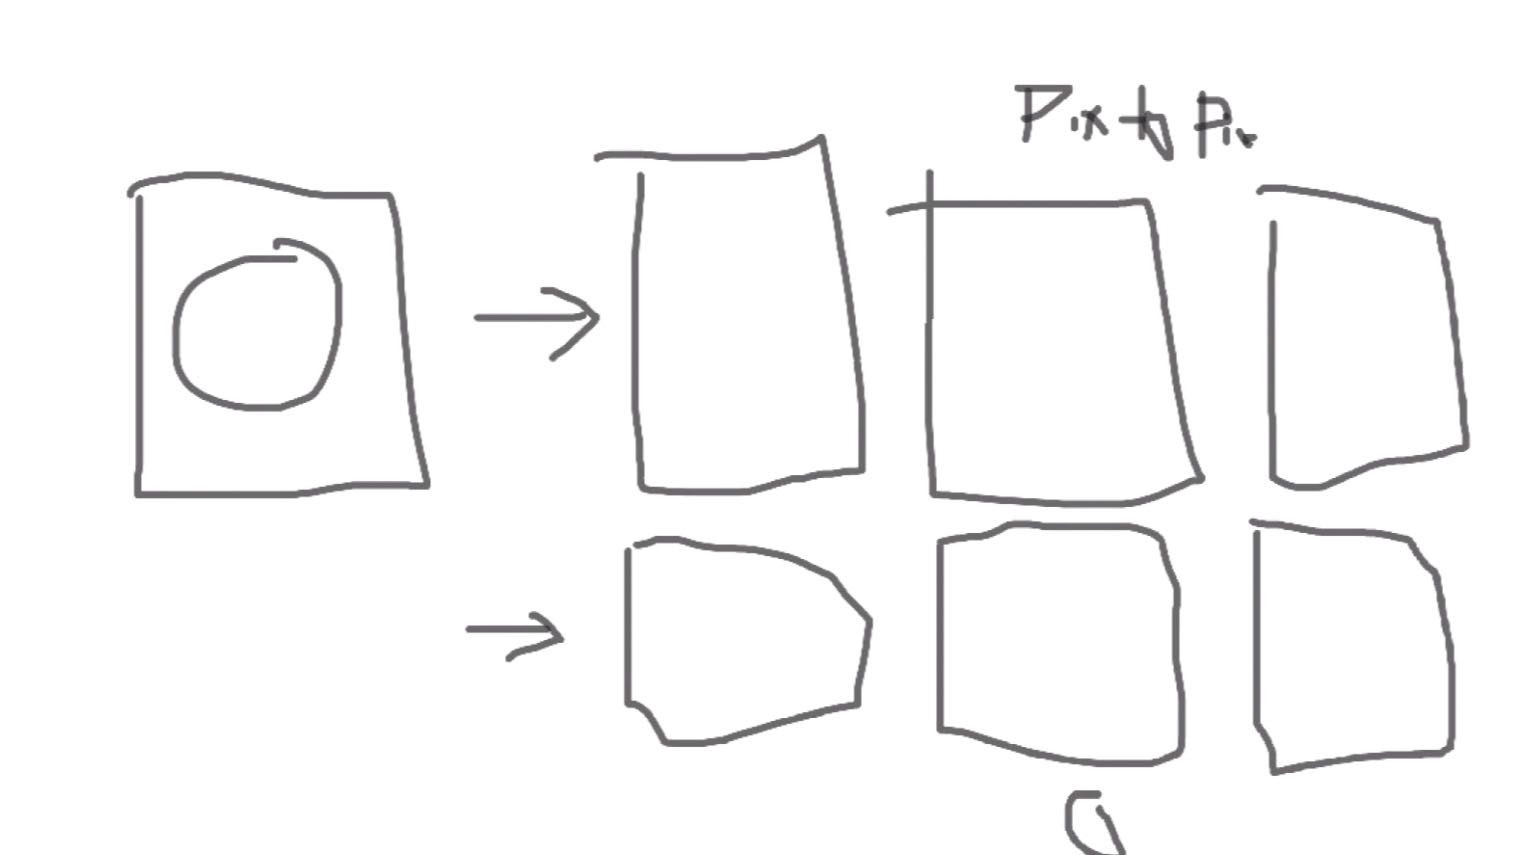
\includegraphics[width=.9\linewidth,height=4.5cm]{images/teaser/sketch.jpg}
%     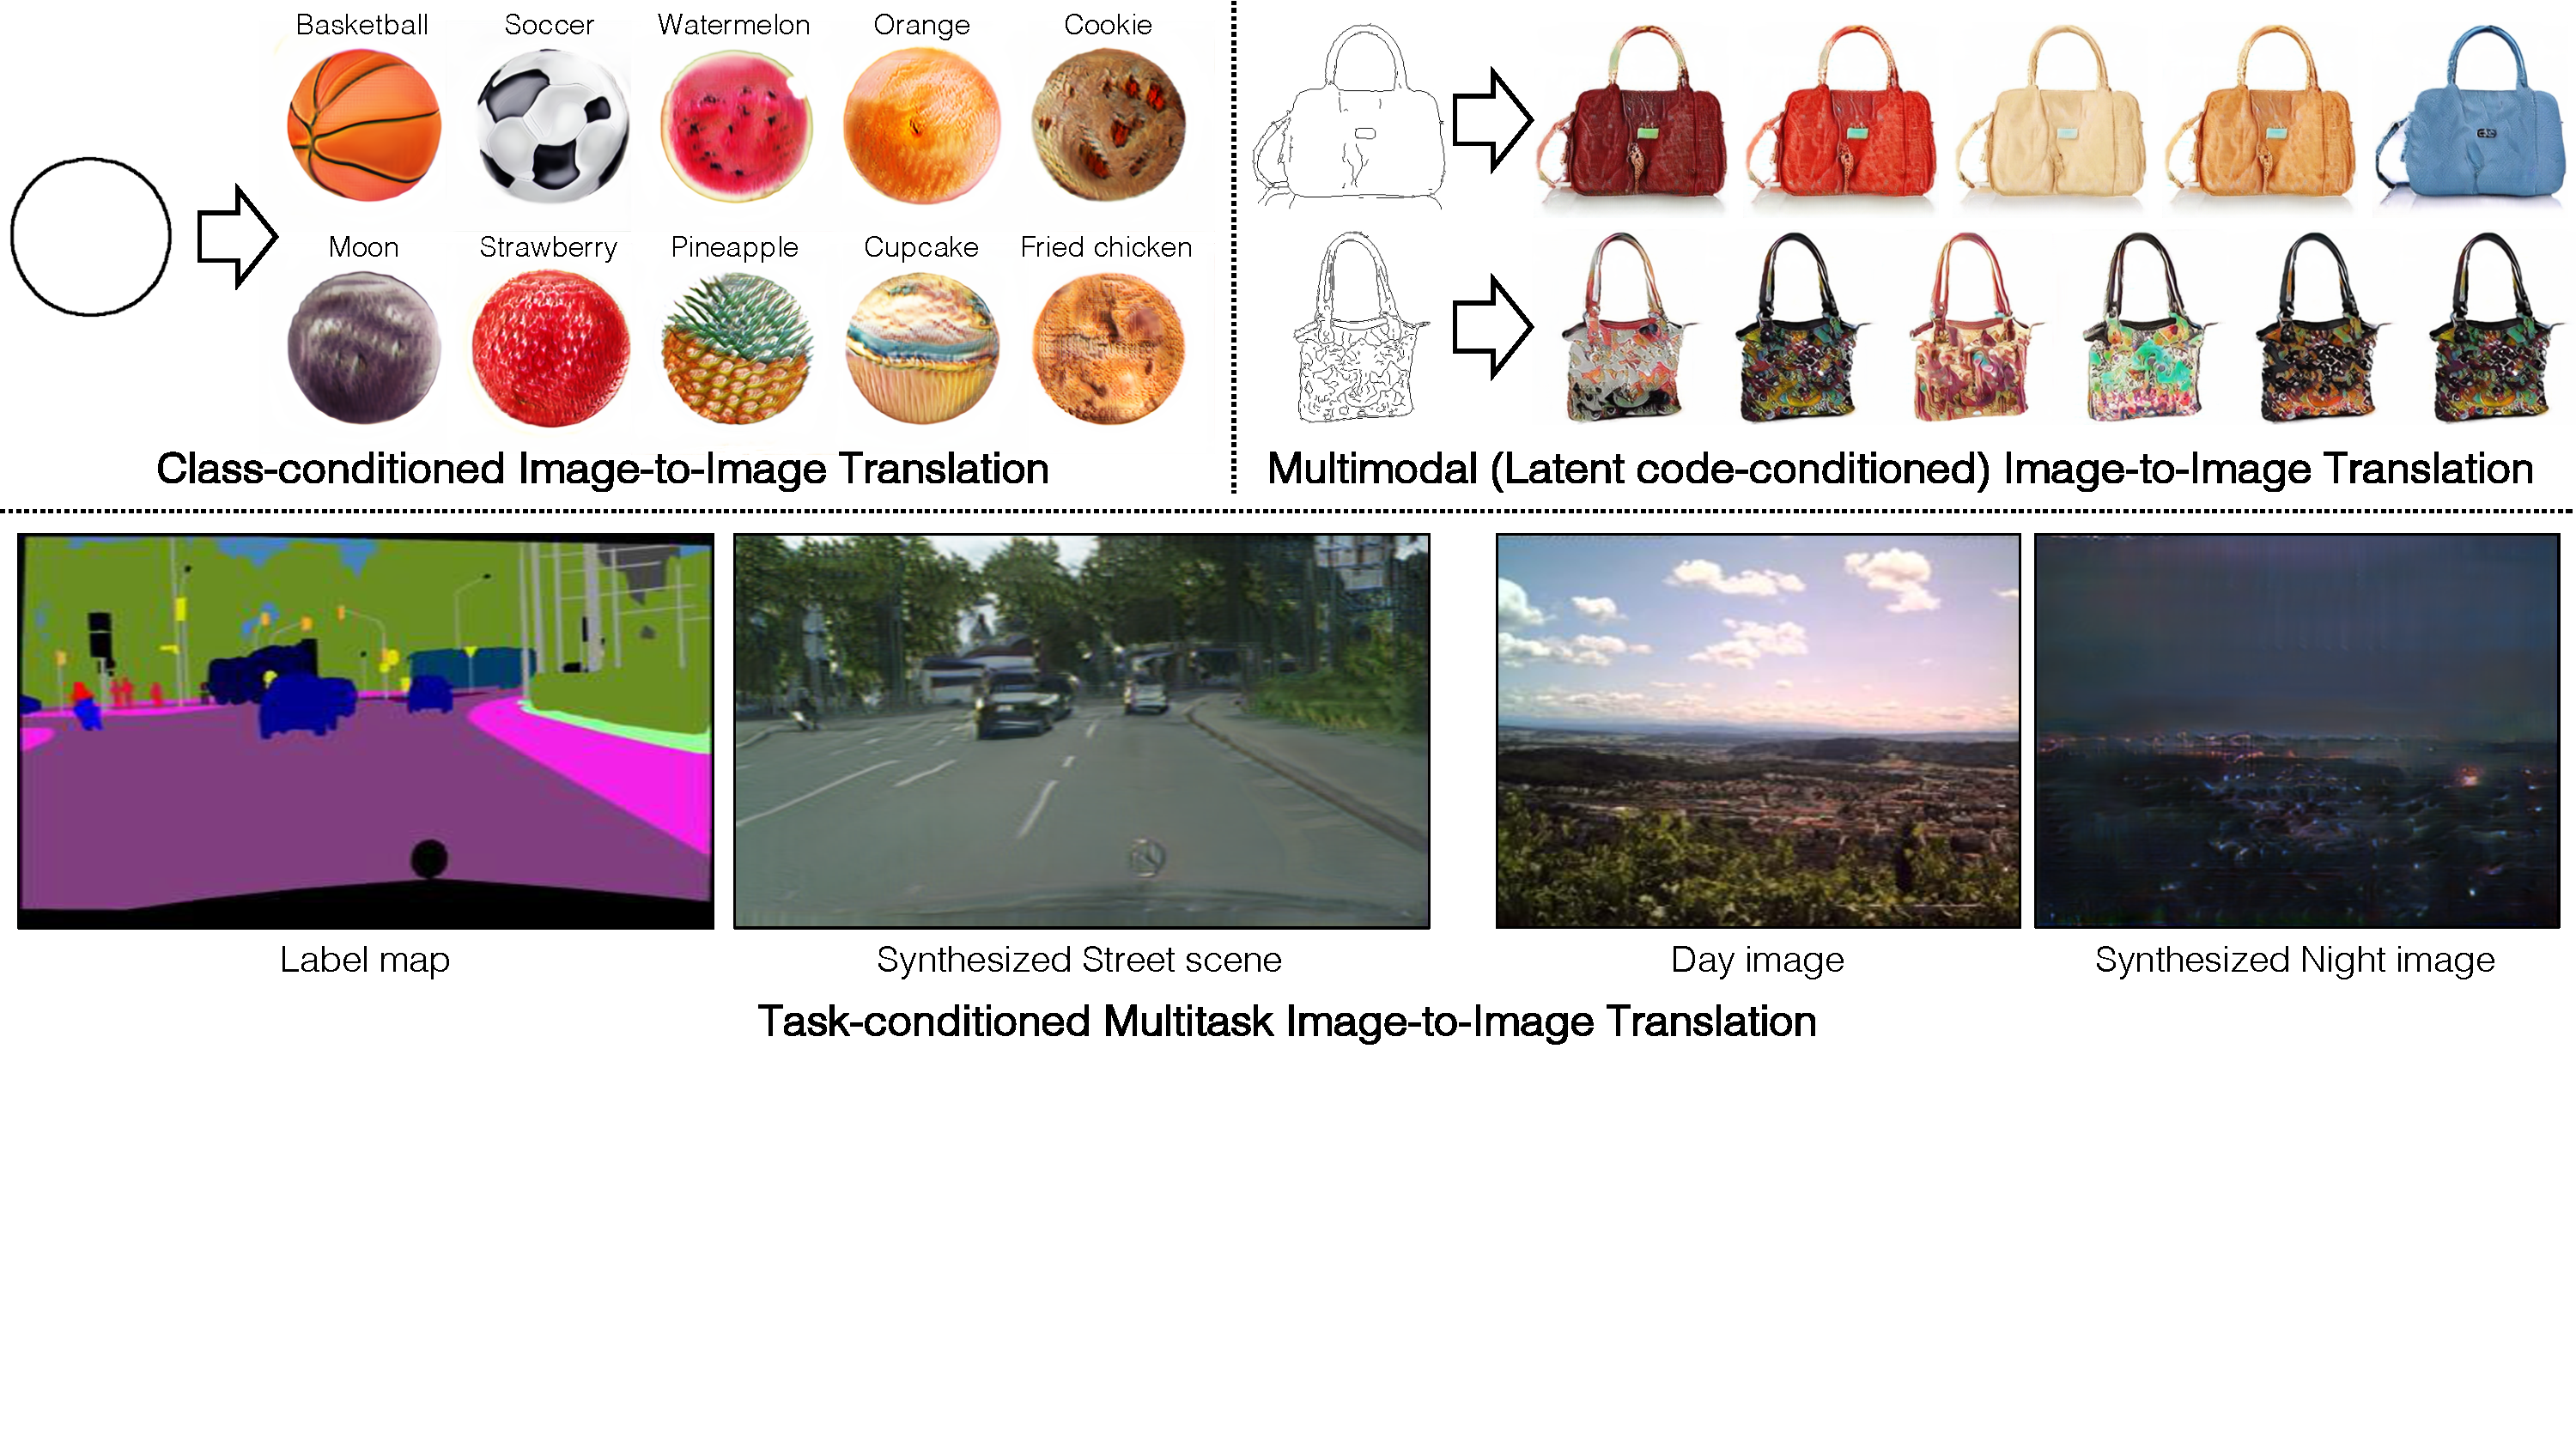
\includegraphics[width=1.\linewidth]{paper_images/fig1.pdf}
%     \captionof{figure}{Our proposed GAN-gate method enables a variety of challenging image-to-image translation tasks, such as {\bf (top-left)} multiclass outline-to-image translation, conditioned on object class {\bf (top-right)} multimodal edge map-to-handbag translation, conditioned on a learned latent code, and {\bf (bottom)} disjoint multitask image-to-image translation, conditioned on task. Each of the three examples uses a single generator and discriminator.\label{fig:teaser}
%     % \vspace{-2mm}
%     }
% \end{center}%
% }]
    

% \section{Supplemental material}


% \subsection{InfoGAN based Model}
% The intuitions gained from the experiments performed for the non-parametric density estimation led to the Gated Residual Block on the Generator of a GAN. InfoGAN \cite{chen2016infogan} presented a perfect setting to apply the Gated Residual Block in the case of the generator. The first set of experiments were on MNIST and Fashion-MNIST with sets of 10 discrete variables (since there were 10 classes in both of the datasets) and 2 continuous variables whose information was tried to be maximized using the Q network. As can be seen in \figref{fig:infogan_unconditional} the network was able to generate realistic images from the different classes and produce meaningful interpolations by varying the continuous variables as shown in the figure. The exact experimental setting was that the hypernetwork responsible for the predictions of the $alpha^i$s which we term as the gate selection network gets the salient variables and has no information about the random noise sampled for the main network(consisting of gated residual blocks), based on the salient variables received the gate selection network predicts the  $alpha^i$s for all the blocks of the network. The main network is oblivious of the conditioning received in the salient variables and has to generate images coherent with the conditioning since the Q-Network tries to reconstruct back the conditioning received in the form of salient variables. 

% \begin{figure}[t]%[ht!]
%     \centering
%     \addSubFigHalf{Picture35}{MNIST}{fig:infogan_mnist} 
%     \addSubFigHalf{Picture34}{Fashion-MNIST}{fig:infogan_fashion_mnist} 
%     \caption{Gated Residual Block-InfoGAN on MNIST and Fashion MNIST \ow{do we have the standard infogan comparison here?}}
%     \label{fig:infogan_unconditional}
%     \vspace{-3mm}
% \end{figure}

% \subsection{Unconditional Generations}
% \begin{figure}[t]
%     \centering
%     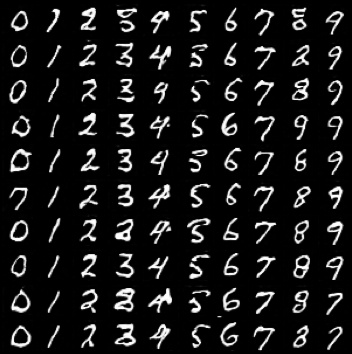
\includegraphics[width=0.5\linewidth]{Picture5}
%     \caption{Results on the Gated Residual Block on MNIST dataset}\label{fig:grb_mnist}
%     \vspace{-4mm}
% \end{figure}

% A well known problem in image conditional GAN settings is the tendency to produce realistic outputs but not being able to produce meaningful variations in the generated output. It was especially prevalent in the original pix2pix setting \cite{isola2016image2image} and further research enabled variations such as \cite{ghosh2017multi} and \cite{zhu2017toward}. Although as shown in \cite{ghosh2017multi} the naive infoGAN setting couldn't produce meaningful variations in the pix2pix setting, settling rather for very minute variations. Our Gated Residual Blocks could mitigate some of the problems and did produce variations in the challenging task of edges-to-bag generation as has been demonstrated in \figref{fig:infogan_bags}. By varying the continuous variable smooth interpolations could be obtained between colors and textures which was earlier not possible with the infogan based pix2pix setting. Although the variations along the discrete axis was quite minimal and we are still investigating the cause for the same. The experimental setting in this scenario was that the salient variables were only given to the gate selection network and had to predict the $alpha^i$s for the main network which consisted of gated residual blocks and was oblivious of the conditioning provided in the form of salient variables. The Discriminator network was the standard image conditional discriminator network while the Q network in this scenario was modified to take the generated image as well as the edge map to behave as a image conditional Q Network which tries to reconstruct back the salient variables given to the gate selection network. 

% \newcommand{\addSubFigEighth}[3]{\begin{subfigure}[t]{.18\linewidth}
%   \includegraphics[width=\linewidth]{#1}
%   \caption{#2}\label{#3}\end{subfigure}
% }
% \newcommand{\addSubFigEighthCaptionless}[3]{\begin{subfigure}[t]{.18\linewidth}
%   \includegraphics[width=\linewidth]{#1}
%   \label{#2}\end{subfigure}
% }

% The next set of experiments were performed to judge the robustness of the Gate Selection Blocks and the Gated Residual Blocks in the case the labels were available. That meant using the gate selection network and the gated residual blocks on the discriminator. The implications were even more interesting, the gate selection network would have to distribute the blocks between the classes to get the class specific gradients back for training the class conditioned generator. In the unconditional setting for the generator, the main block only receives random noise and the gate selection block receives the class condition and predicts the $aplha^i$s for the gated residual blocks. The discriminator on the other hand is composed of a main network consisting of gated residual blocks which is oblivious to the class conditioning and a gate selection network which predicts the $aplha^i$s for the main network of the discriminator. The main network predicts how real/fake an image is based on the alpha weightings of its gated residual blocks. The network is able to disentangle the class conditioning although none of the main networks of the generator/ discriminator are aware of the class conditioning, the class information only being input to the gate selection network which has to modulate the weights of the respective networks' gated residual blocks. The generated samples on the MNIST dataset are shown in \figref{fig:grb_mnist} and the alpha gatings for the different classes and the different blocks in \figref{fig:mnist_act}. The values for the gates clearly show switching off of certain blocks in the case it is not needed for a particular class even though a sparsity constraint was not applied in the training objective.


% \begin{figure}%[ht!]
%     \centering
%     \addSubFigHalf{Picture6}{Activations of the gated residual blocks in the generator}{fig:gen_act} 
%     \addSubFigHalf{Picture7}{Activations of the gated residual blocks in the discriminator}{fig:dis_act} 
%     \caption{Activation of the various blocks in the Generator and Discriminator}
%     \label{fig:mnist_act}
%     \vspace{-3mm}
% \end{figure}






% \begin{figure*}[t]%[ht!]
%     \centering
%     \addSubFigEighthCaptionless{Picture8}{Sketch}{fig:bag_sketch} 
%     \addSubFigEighthCaptionless{Picture9}{Varition 1}{fig:bag_1} 
%     \addSubFigEighthCaptionless{Picture10}{Varition 2}{fig:bag_2}
%     \addSubFigEighthCaptionless{Picture11}{Varition 3}{fig:bag_3}
%     \addSubFigEighthCaptionless{Picture12}{Varition 4}{fig:bag_4}
%     \caption{The variations produced in the sketch to realistic bag task in the infogan with Gated Residual Block setting for the generator }
%     \label{fig:infogan_bags}
%     \vspace{-3mm}
% \end{figure*}

\begin{figure*}[t]
    \centering
    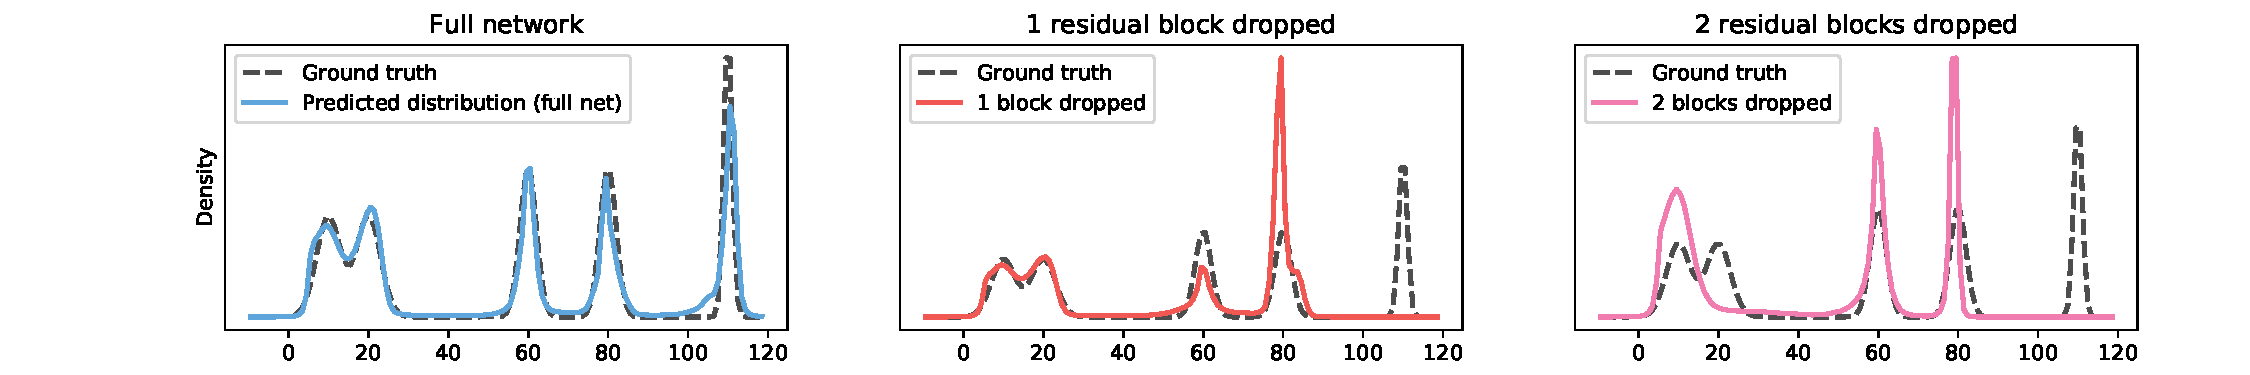
\includegraphics[width=\linewidth,trim={2.6cm 0 1.8cm 0},clip]{paper_images/mog.pdf}
    % 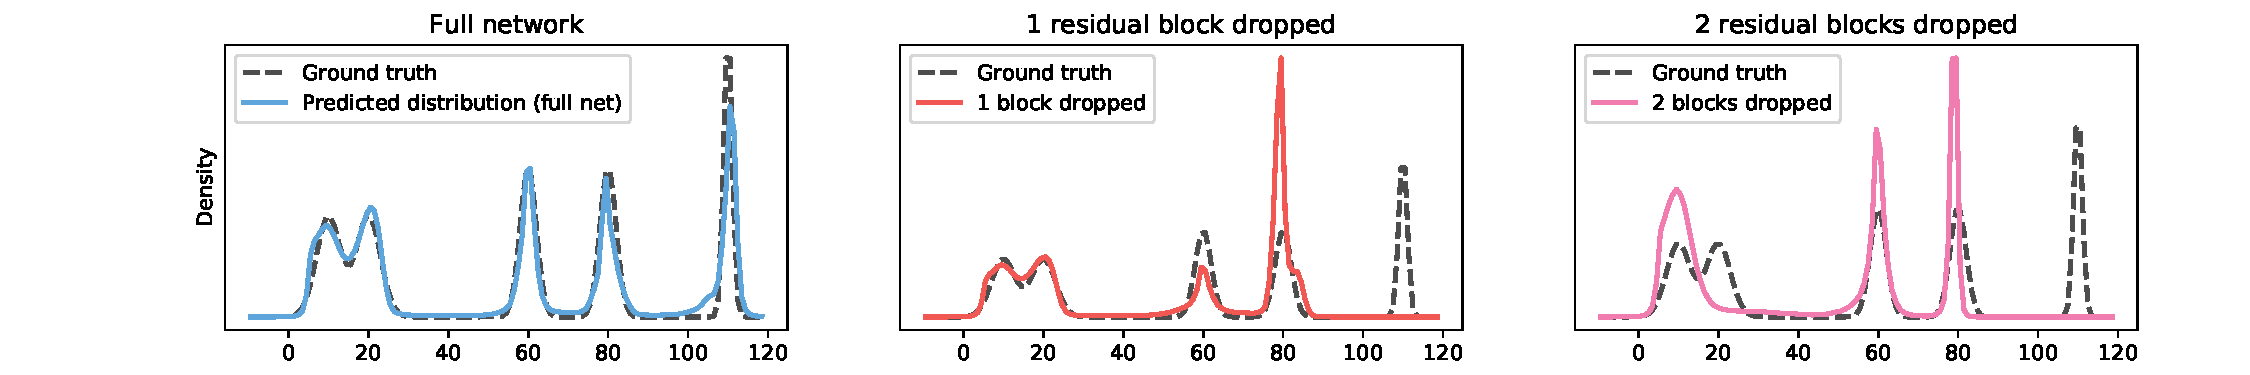
\includegraphics[width=\linewidth]{paper_images/mog.pdf}
    \caption{{\bf 1D Mixture of Gaussians.} {\bf (Left)} Samples from a residual network (blue-dotted) closely approximate the training distribution (black). {\bf (Mid)} Removing one residual block removes one mode of the predicted distribution. {\bf (Right)} Removing two blocks drops two modes. Note that samples stay mostly ``on-manifold" of the ground truth distribution. {\bf Note:} This is a reproduction of Figure 2 from the main paper, it is included here for completeness.
    \vspace{-2mm}
    }\label{fig:onedexperiment}
    \vspace{-3mm}
\end{figure*}

\section{1D Mixture of Gaussians Dataset}
% In order to understand the behavior of the various residual blocks, we first perform a very simple synthetic experiment, much easier than generating high-dimensional complex images.
We consider a 1D mixture of Gaussians with five components with modes at 10, 20, 60, 80 and 110, and standard deviations of 3, 3, 2, 2 and 1, respectively. While the first two modes overlap significantly, the fifth mode stands isolated as shown in \figref{fig:onedexperiment}. We train our Resnet block based GAN model using 1 million samples from this distribution and generate 1 million samples from the trained model. In order to compare the learned distribution with the ground truth distributions, we estimate the learned distribution by computing histograms over the data points. 
%These histograms are carefully created using different bin sizes and the best bin (found to be 0.1) is chosen. 
%The generated distribution from the trained model corresponds very closely to the ground truth distribution. 
As shown in \figref{fig:onedexperiment}, the generated distribution closely matches the ground truth one, and we can observe that  residual blocks focus on specific modes, which motivates our gating mechanism.


\section{1D Network Architecture}
% \ow{but why was this architecture chosen? did the normal ones in madgan/mode gan not work? what motivates the skinny resnet?} 
The architecture was designed hoping to reproduce some of the experiments performed by \cite{veit2016residual} by removal of blocks and observing the resulting generated distribution, hence a design choice of having a deep network but keeping the neurons in each block lesser in order to reduce chances of overfitting/overparametrizing for a relatively simpler task. The interesting aspect was that although the network was deeper (16 layers of residual blocks) than required for similar experiments in MAD-GAN \cite{ghosh2017multi}, Mode Regularized GAN \cite{che2016mode} and Unrolled GAN \cite{metz2017unrolledGAN}, there were only 4 neurons in each residual block of the generator and discriminator (Tables~\ref{table:1d_G}~\&~\ref{table:1d_D}) compared to fully connected versions in which there consisted of connections between 256 neurons in the preceding layer to 256 neurons in the current layer. Thus although the number of parameters were much less, the network learned the distribution quite accurately. The architecture used in this experiment inspired the design of the skinny Resnet architecture as described later.

\begin{table}[ht]
\caption{\textbf{ResBlock}} % title of Table
\centering % used for centering table
\begin{tabular}{c} % centered columns (4 columns)
\toprule
\textbf{F(x)}\\\midrule
Linear\\ % inserting body of the table
ReLU() \\
Linear\\
\bottomrule %inserts single line
\end{tabular}
\label{table:resblock} % is used to refer this table in the text
\end{table}

\begin{table}[ht]
\caption{\textbf{Generator for 1D setting}} % title of Table
\centering % used for centering table
\begin{tabular}{l c c}
%  \hline
\toprule
\textbf{Layer} & \textbf{Neurons} & \textbf{Num Layers} \\ \midrule
Linear & 10 $\rightarrow$ 4 & 1  \\ %\midrule
ResBlock & 4 & 16 \\ 
Linear & 4$\rightarrow$ 1 & 1 \\ 
\bottomrule %inserts single line
\end{tabular}
\label{table:1d_G} % is used to refer this table in the text
\end{table}

% \begin{table}[ht]
% \caption{\textbf{Generator for 1D setting}} % title of Table
% \centering % used for centering table
% \begin{tabular}{c c} % centered columns (4 columns)
% \hline\hline %inserts double horizontal lines
% layer & num layers\\%heading
% \hline % inserts single horizontal line
% Linear(10,4) & 1\\ % inserting body of the table
% ResBlock(4) & 16 \\
% Linear(4,1) & 1 \\
% \hline %inserts single line
% \end{tabular}
% \label{table:1d_G} % is used to refer this table in the text
% \end{table}

% \begin{table}[ht]
% \caption{\textbf{Discriminator for 1D setting}} % title of Table
% \centering % used for centering table
% \begin{tabular}{c c} % centered columns (4 columns)
% \hline\hline %inserts double horizontal lines
% layer & num layers\\%heading
% \hline % inserts single horizontal line
% Linear(1,4) & 1\\ % inserting body of the table
% ResBlock(4) & 16 \\
% Linear(4,1) & 1 \\
% Sigmoid & 1 \\
% \hline %inserts single line
% \end{tabular}
% \label{table:1d_D} % is used to refer this table in the text
% \end{table}

\begin{table}[ht]
\caption{\textbf{Discriminator for 1D setting}} % title of Table
\centering % used for centering table
\begin{tabular}{l c c}
%  \hline
\toprule
\textbf{Layer} & \textbf{Neurons} & \textbf{Num Layers} \\ \midrule
Linear & 1 $\rightarrow$ 4 & 1  \\ %\midrule
ResBlock & 4 & 16 \\ 
Linear & 4 $\rightarrow$ 1 & 1 \\
Sigmoid & 1 & 1 \\
\bottomrule %inserts single line
\end{tabular}
\label{table:1d_D} % is used to refer this table in the text
\end{table}


\section{Outline$\rightarrow$Image Network Architecture}
The network architecture is based on our observations that deeper networks perform better capturing multi-modal data distributions. The second guiding principle in the design of the architecture is that the different blocks should have similar number of channels so that the gating hypernetwork can distribute the modes between the blocks efficiently. Finally, the residual blocks responsible for upsampling and downsampling were gated as well in order to allow more blocks to be gated and hence better fine-grained control on the generation process. 
\tabref{table:convresblock} shows the Convolution Residual Block which does not change the spatial resolution of the activation volume, 
\tabref{table:downconvresblock} shows the Downsampling Residual Block which reduces the activation volume to half the spatial resolution, 
\tabref{table:upconvresblock} shows the Upsampling Residual Block which increases the activation volume to twice the spatial resolution,  and in the case of gating (either block wise/channel-wise) the gating is applied on the $F(x)$ of each network. 
The shortcut branch represented in \tabref{table:upconvresblock} and \tabref{table:downconvresblock} represents the branch of the Resnet which is added to $F(x)$ branch. In these scenarios since the resolution of $x$ changes in $F(x)$ branch hence the shortcut also has a similar upsampling/downsampling layer.


\begin{table}[ht]
    \makegapedcells
        \centering % used for centering table
        \begin{tabular}{c} % centered columns (4 columns)
        % \hline\hline %inserts double horizontal lines
        \toprule
        \textbf{F(x)}\\%heading
        \midrule
        Conv2d \\
        InstanceNorm\\ % inserting body of the table
        ReLU() \\
        Conv2d \\
        InstanceNorm\\ % inserting body of the table
        ReLU() \\
        \bottomrule %inserts single line
        \end{tabular}
        \caption{\textbf{ConvResblock}} % title of Table
        \label{table:convresblock} % is used to refer this table in the text
\end{table}

\begin{table}
        \centering % used for centering table
        \begin{tabular}{c} % centered columns (4 columns)
        \toprule % \hline\hline %inserts double horizontal lines
        \textbf{F(x)}\\%heading
        \midrule % \hline
        Upsample (Nearest Neighbor) \\
        ReflectionPad \\
        Conv2d \\
        InstanceNorm\\ % inserting body of the table
        ReLU() \\
        Conv2d \\
        InstanceNorm\\ % inserting body of the table
        ReLU() \\
        \midrule % \hline %inserts single line
        \textbf{Shortcut Branch}\\
        \midrule % \hline 
        Upsample (Bilinear) \\
        ReflectionPad\\
        Conv2d \\
        \bottomrule % \hline
        \end{tabular}
        \caption{        \label{table:upconvresblock} \textbf{UpConvResblock}} % title of Table
\end{table}

\begin{table}
        \centering % used for centering table
        \begin{tabular}{c} % centered columns (4 columns)
        \toprule % \hline\hline %inserts double horizontal lines
        \textbf{F(x)}\\%heading
        \midrule
        Avgpool 2d \\
        ReflectionPad \\
        Conv2d \\
        InstanceNorm\\ % inserting body of the table
        ReLU() \\
        Conv2d \\
        InstanceNorm\\ % inserting body of the table
        ReLU() \\
        \midrule% \hline %inserts single line
        \textbf{Shortcut Branch}\\
        \midrule % \hline 
        Avgpool 2d \\
        ReflectionPad\\
        Conv2d \\
        \bottomrule% \hline
        \end{tabular}
        \caption{\label{table:downconvresblock} \textbf{DownConvResblock}} 
\end{table}


\begin{table}[ht]
\caption{\textbf{Gated Resnet G:Scribble Dataset}}
\centering % used for centering table
\begin{tabular}{l c c} % centered columns (4 columns)
\toprule% \hline
\textbf{Layer} & \textbf{Filter} & \textbf{Num Layers} \\
\midrule
Conv2d & 3 $\rightarrow$ 32 & 1\\
InstanceNorm & 32 & 1 \\ % inserting body of the table
ReLU() & 32 & 1\\
\hdashline% \hline %inserts single line
\textbf{Gated}-ConvResBlock & 32 & 3\\
\textbf{Gated}-DownConvResBlock & 32 & 3\\
\textbf{Gated}-ConvResBlock & 32 & 12\\
\textbf{Gated}-UpConvResBlock & 32 & 3\\
\textbf{Gated}-ConvResBlock & 32 & 3\\
\hdashline
Conv2d & 32$\rightarrow$3 & 1 \\
Tanh() & 3 & 1 \\
\bottomrule% \hline
\end{tabular}
\label{table:resnet_g_scribble} % is used to refer this table in the text
\end{table}

\begin{table}[ht]
\caption{\textbf{Gated Resnet D:Scribble Dataset}}
\centering % used for centering table
\begin{tabular}{l c c} % centered columns (4 columns)
\toprule% \hline
\textbf{Layer} & \textbf{Filter} & \textbf{Num Layers} \\
\midrule
Conv2d & 6 $\rightarrow$ 32 & 1\\
\hdashline% \hline %inserts single line
\textbf{Gated}-ConvResBlock & 32 & 3\\
\textbf{Gated}-DownConvResBlock & 32 & 4\\
\textbf{Gated}-ConvResBlock & 32 & 17\\
\hdashline
Conv2d & 32$\rightarrow$1 & 1 \\
Sigmoid() & 1 & 1 \\
\bottomrule% \hline
\end{tabular}
\label{table:resnet_d_scribble} % is used to refer this table in the text
\end{table}


\begin{table}[ht]
\caption{\textbf{Gated Resnet G:Multi-Task Dataset}}
\centering % used for centering table
\begin{tabular}{l c c} % centered columns (4 columns)
\toprule% \hline
\textbf{Layer} & \textbf{Filter} & \textbf{Num Layers} \\
\midrule
Conv2d & 3 $\rightarrow$ 64 & 1\\
InstanceNorm & 64 & 1 \\ % inserting body of the table
ReLU() & 64 & 1\\
\hdashline% \hline %inserts single line
\textbf{Gated}-ConvResBlock & 64 & 3\\
\textbf{Gated}-DownConvResBlock & 64 & 3\\
\textbf{Gated}-ConvResBlock & 64 & 4\\
\textbf{Gated}-UpConvResBlock & 64 & 3\\
\textbf{Gated}-ConvResBlock & 64 & 3\\
\hdashline
Conv2d & 64$\rightarrow$3 & 1 \\
Tanh() & 3 & 1 \\
\bottomrule% \hline
\end{tabular}
\label{table:resnet_g_multitask} % is used to refer this table in the text
\end{table}

\begin{table}[ht]
\caption{\textbf{Gated Resnet D:Multi-Task Dataset}}
\centering % used for centering table
\begin{tabular}{l c c} % centered columns (4 columns)
\toprule% \hline
\textbf{Layer} & \textbf{Filter} & \textbf{Num Layers} \\
\midrule
Conv2d & 6 $\rightarrow$ 64 & 1\\
\hdashline% \hline %inserts single line
\textbf{Gated}-ConvResBlock & 64 & 3\\
\textbf{Gated}-DownConvResBlock & 64 & 4\\
\textbf{Gated}-ConvResBlock & 64 & 9\\
\hdashline
Conv2d & 64$\rightarrow$1 & 1 \\
Sigmoid() & 1 & 1 \\
\bottomrule% \hline
\end{tabular}
\label{table:resnet_d_multitask} % is used to refer this table in the text
\end{table}


\subsection{Gating Hypernetwork:}
The gating hypernetwork was also designed using Resnet blocks, we used 1D convolutions in the Resnet block \tabref{table:resblock1D} to reduce the number of parameters and to use BatchNormalization to speed up the training of the network responsible for the prediction of gating. The class conditioning is first passed through an embedding layer to obtain a representation of the class which could be further processed by the Resnet blocks. The same network is used for the various forms of gating. In case of block wise gating the number of outputs $dim^{gate}$ for this network is equal to the number of blocks used in the main network, in the case of an affine transformation the network predicts an equal number of biases for each of the block. In case of channel-wise gating the number of predicted parameters $dim^{gate}$ is equal to $num^{channels}\times num^{blocks}$ since each residual block consists of equal number of channels in each it helps to ease the training of the gating hypernetwork. The $\alpha$ was constrained between 0 and 1 to mimic whether to select a block or to reject the block while the $\beta$ in the case of affine transformation was restricted between -1 and 1. In the case of standard AdaIN, the parameters are unrestricted but it did not work in that setting and the AdaIN parameters had to be constrained between -1 and 1 in order for the network to perform well. 

\begin{table}[ht]
\caption{\textbf{ResBlock1D}} % title of Table
\centering % used for centering table
\begin{tabular}{c} % centered columns (4 columns)
\toprule
\textbf{F(x)}\\\midrule
Conv1D\\ % inserting body of the table
BatchNorm1D\\
ReLU \\
Conv1D\\
BatchNorm1D\\
ReLU \\
\bottomrule %inserts single line
\end{tabular}
\label{table:resblock1D} % is used to refer this table in the text
\end{table}

\begin{figure*}[t]
    \centering
    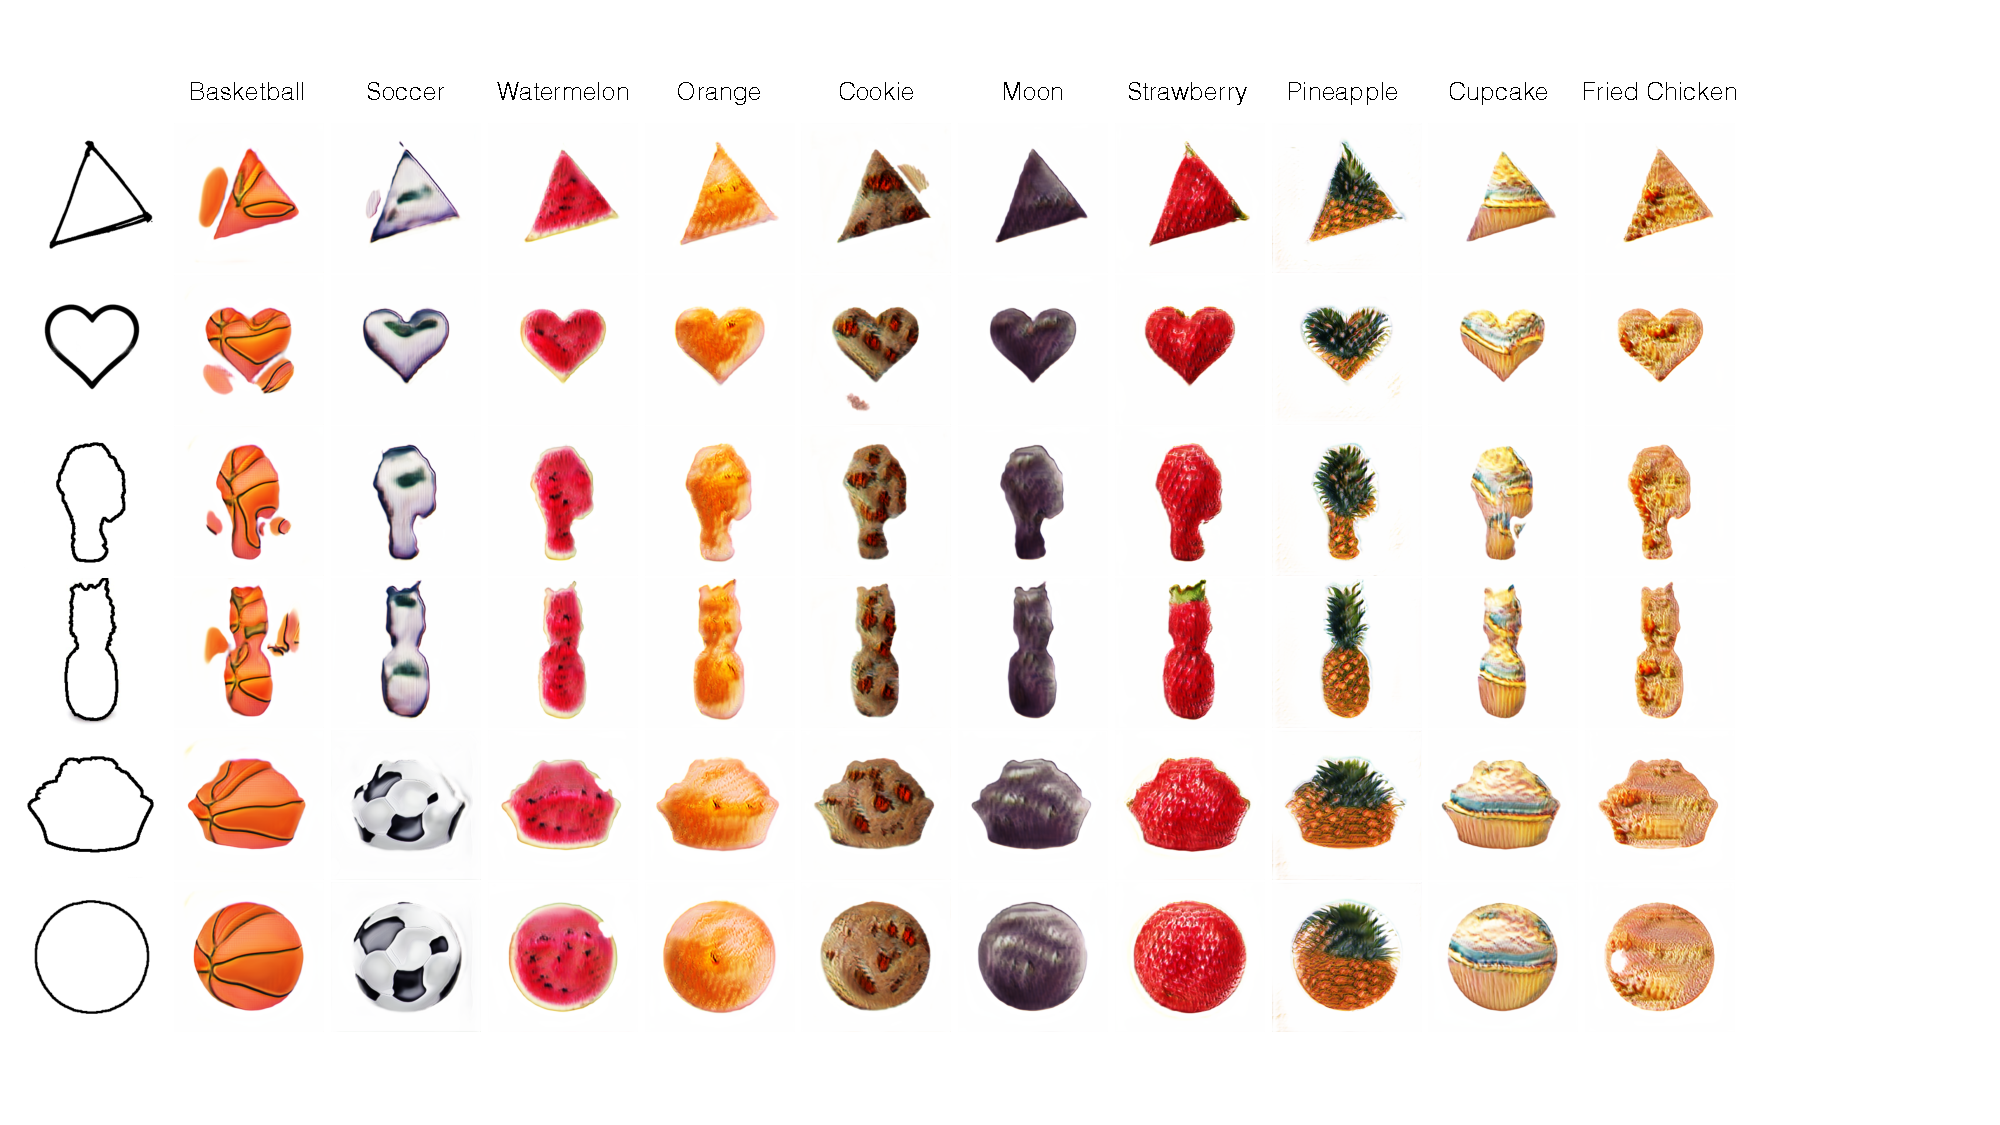
\includegraphics[width=\linewidth,trim={0 0 4.5cm 0},clip]{paper_images/supplementary_grid_channel.pdf}
    % 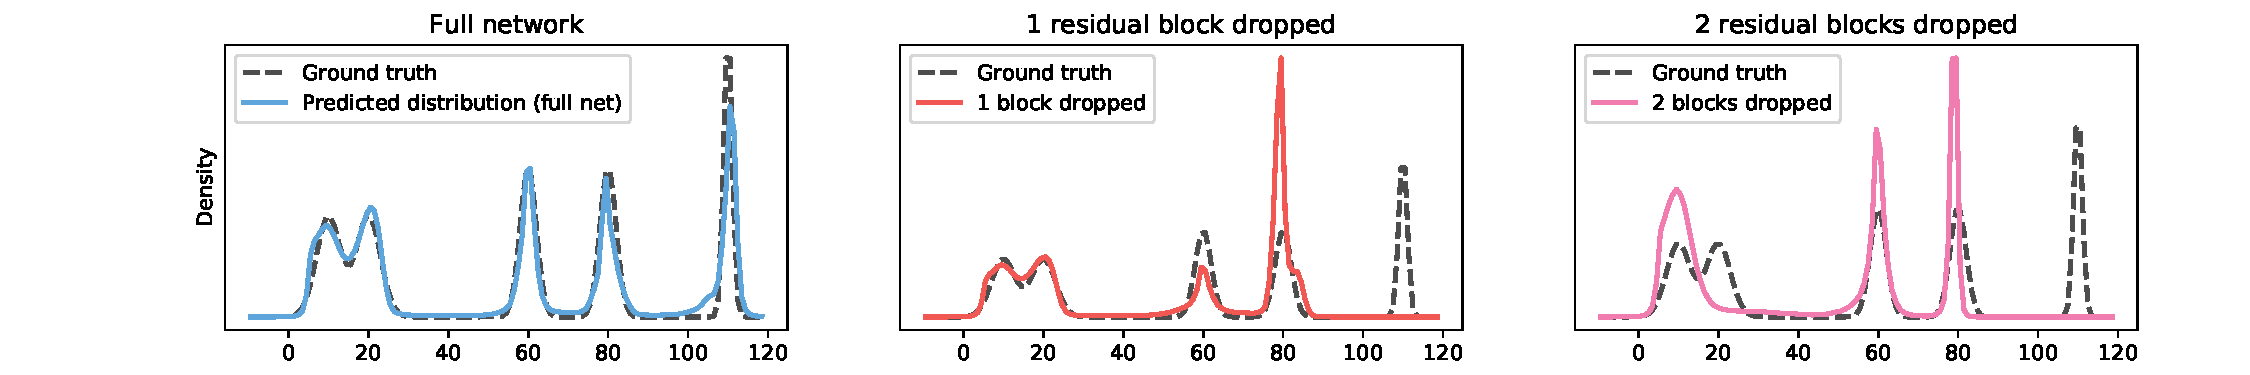
\includegraphics[width=\linewidth]{paper_images/mog.pdf}
    \caption{{\bf Channel-Wise Gating:} We observe that the technique extends to not only the shapes it was trained on but can also generate images for some input shapes corresponding to other classes and to the extreme can generate images for certain shapes it never encountered during training such as the triangle and heart were directly downloaded from the internet. }
    \label{fig:channel_shapes}
    \vspace{-3mm}
\end{figure*}


\begin{table}[ht]
\caption{\textbf{Gating Hyper Network} $dim^{gate}$ is the number of blocks in the case of Block Wise Gating and the number of channels in the case of Channel Wise Gating. In case of affine its twice of each since the $\beta$ is of the same dimension }
\centering % used for centering table
\begin{tabular}{l c c} % centered columns (4 columns)
\toprule% \hline
\textbf{Layer} & \textbf{Filter/Shape} & \textbf{Num Layers} \\
\midrule
Embedding & $dim^{embed}$ & 1 \\
Conv1d & 1 $\rightarrow$ 16 & 1\\
% \hdashline% \hline %inserts single line
ResBlock1D & 16 & 16\\
Reshape & 16$\times dim^{embed}$ & 1\\
Linear & 16$\times dim^{embed} \rightarrow dim^{gate} $& 1\\
\bottomrule% \hline
\end{tabular}
\label{table:resnet_gating} % is used to refer this table in the text
\end{table}

\section{InfoGAN with Variations:}
The network architectures used in this setting are very similar to the ones used for the outline $\rightarrow$ image generation with some small differences. The discriminator and the Q network responsible for the maximization of mutual information are not gated in this case since the class labels are not provided to the discriminator or the Q network. The number of blocks and channels in each block in the case of the generator are more than the case of scribble dataset. The gating hypernetwork also differs slightly since the sampled variables are not only one-hot encoding but a combination of one-hot and gaussian variables, hence we directly use it and bypass the embedding layer.

\begin{table}[ht]
\caption{\textbf{Gating Hyper Network(InfoGAN)}
% nsalient(12) are the number of variables representing
We have $C=2$ continuous and $K=10$ discrete latent variables. Variable $dim^{gate}$ is the number of channels which are gated. }
\centering % used for centering table
\begin{tabular}{l c c} % centered columns (4 columns)
\toprule% \hline
\textbf{Layer} & \textbf{Filter/Shape} & \textbf{Num Layers} \\
\midrule
Reshape & $K+C$ & 1 \\
Conv1d & 1 $\rightarrow$ 16 & 1\\
% \hdashline% \hline %inserts single line
ResBlock1D & 16 & 16\\
Reshape & $16\times (K+C)$ & 1\\
Linear & $16\times (K+C) \rightarrow dim^{gate} $& 1\\
\bottomrule% \hline
\end{tabular}
\label{table:resnet_gating_infogan} % is used to refer this table in the text
\end{table}

\begin{table}[ht]
\caption{\textbf{Gated Resnet G:InfoGAN}}
\centering % used for centering table
\begin{tabular}{l c c} % centered columns (4 columns)
\toprule% \hline
\textbf{Layer} & \textbf{Filter} & \textbf{Num Layers} \\
\midrule
Conv2d & 3 $\rightarrow$ 64 & 1\\
InstanceNorm & 64 & 1 \\ % inserting body of the table
ReLU() & 64 & 1\\
\hdashline% \hline %inserts single line
\textbf{Gated}-ConvResBlock & 64 & 3\\
\textbf{Gated}-DownConvResBlock & 64 & 3\\
\textbf{Gated}-ConvResBlock & 64 & 20\\
\textbf{Gated}-UpConvResBlock & 64 & 3\\
\textbf{Gated}-ConvResBlock & 64 & 3\\
\hdashline
Conv2d & 64$\rightarrow$3 & 1 \\
Tanh() & 3 & 1 \\
\bottomrule% \hline
\end{tabular}
\label{table:resnet_g_infogan} % is used to refer this table in the text
\end{table}


\begin{table}[ht]
\caption{\textbf{Resnet D:Infogan}}
\centering % used for centering table
\begin{tabular}{l c c} % centered columns (4 columns)
\toprule% \hline
\textbf{Layer} & \textbf{Filter} & \textbf{Num Layers} \\
\midrule
Conv2d & 6 $\rightarrow$ 64 & 1\\
\hdashline% \hline %inserts single line
ConvResBlock & 64 & 3\\
DownConvResBlock & 64 & 4\\
ConvResBlock & 64 & 25\\
\hdashline
Conv2d & 64$\rightarrow$1 & 1 \\
Sigmoid() & 1 & 1 \\
\bottomrule% \hline
\end{tabular}
\label{table:resnet_d_infogan} % is used to refer this table in the text
\end{table}

\begin{table}[ht]
\caption{\textbf{Resnet Q:Infogan}}
\centering % used for centering table
\begin{tabular}{l c c} % centered columns (4 columns)
\toprule% \hline
\textbf{Layer} & \textbf{Filter/Shape} & \textbf{Num Layers} \\
\midrule
Conv2d & 6 $\rightarrow$ 64 & 1\\
\hdashline% \hline %inserts single line
ConvResBlock & 64 & 3\\
DownConvResBlock & 64 & 4\\
ConvResBlock & 64 & 25\\
\hdashline
Conv2d & 64$\rightarrow$1 & 1 \\
Reshape & 225 & 1 \\
\midrule
\textbf{Discrete Branch} \\
\midrule
Linear & 225 $\rightarrow$ 10 & 1 \\
\midrule
\textbf{Continuous Branch($\mu$)} \\
\midrule
Linear & 225 $\rightarrow$ 2 & 1 \\
\midrule
\textbf{Continuous Branch($\sigma$)} \\
\midrule
Linear & 225 $\rightarrow$ 2 & 1 \\
\bottomrule% \hline
\end{tabular}
\label{table:resnet_q_infogan} % is used to refer this table in the text
\end{table}

% \begin{table}[ht]
% \caption{\textbf{Gated Resnet D:Scribble Dataset}} % title of Table
% \centering % used for centering table
% \begin{tabular}{c} % centered columns (4 columns)
% \hline
% Conv2d(6,64,kernel=3,stride=1,padding=1) \\
% \hline %inserts single line
% 3xGatedConvResBlock(64) \\
% 4xDownGatedConvResBlock(64) \\
% 17xGatedConvResBlock(64) \\
% \hline
% Conv2d(64,1,kernel=3,stride=1,padding=1) \\
% Sigmoid() \\
% \hline
% \end{tabular}
% \label{table:resnet_d_scribble} % is used to refer this table in the text
% \end{table}

\section{Unusual Shapes for Various Classes:}

\begin{figure*}[t]
    \centering
    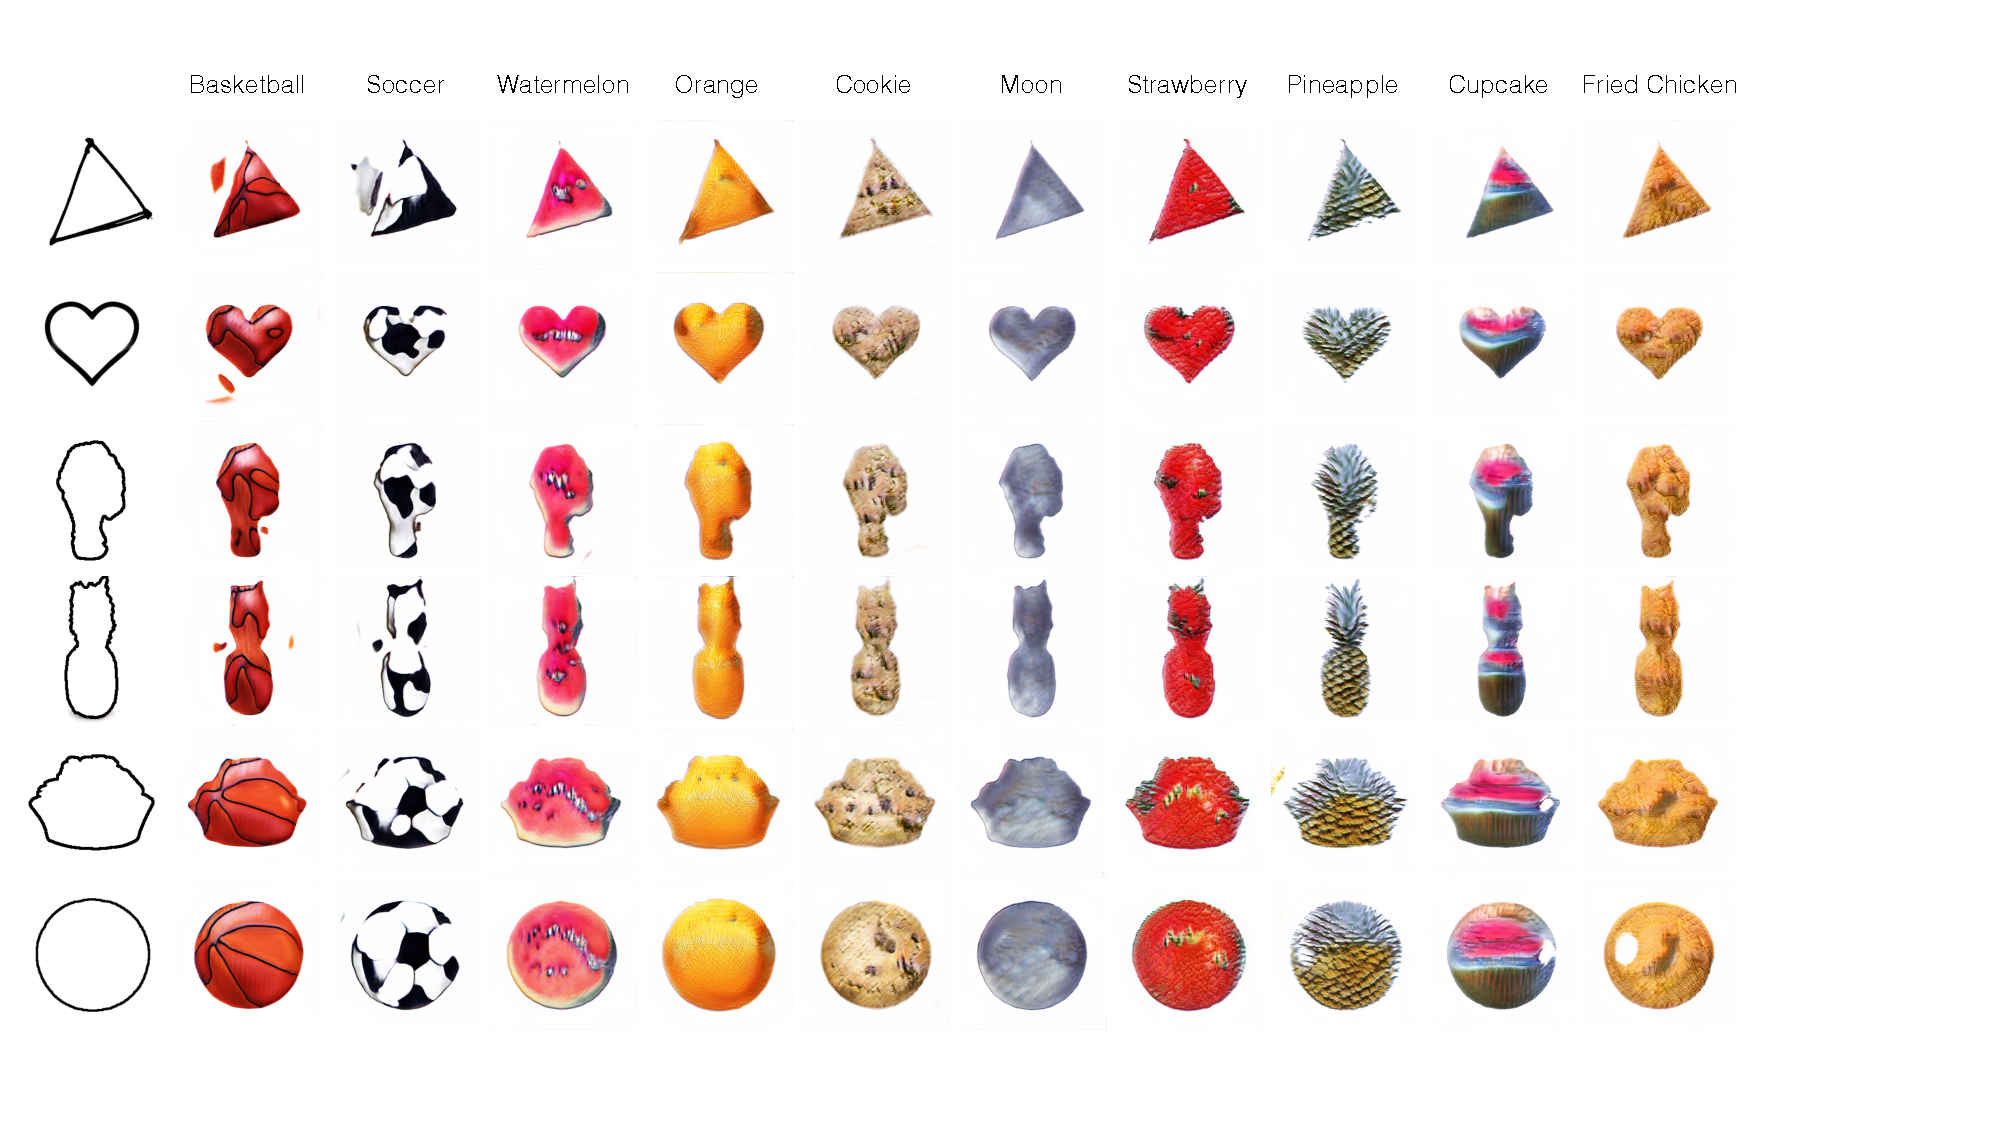
\includegraphics[width=\linewidth,trim={0 0 4.5cm 0},clip]{paper_images/supplementary_grid_block.pdf}
    % 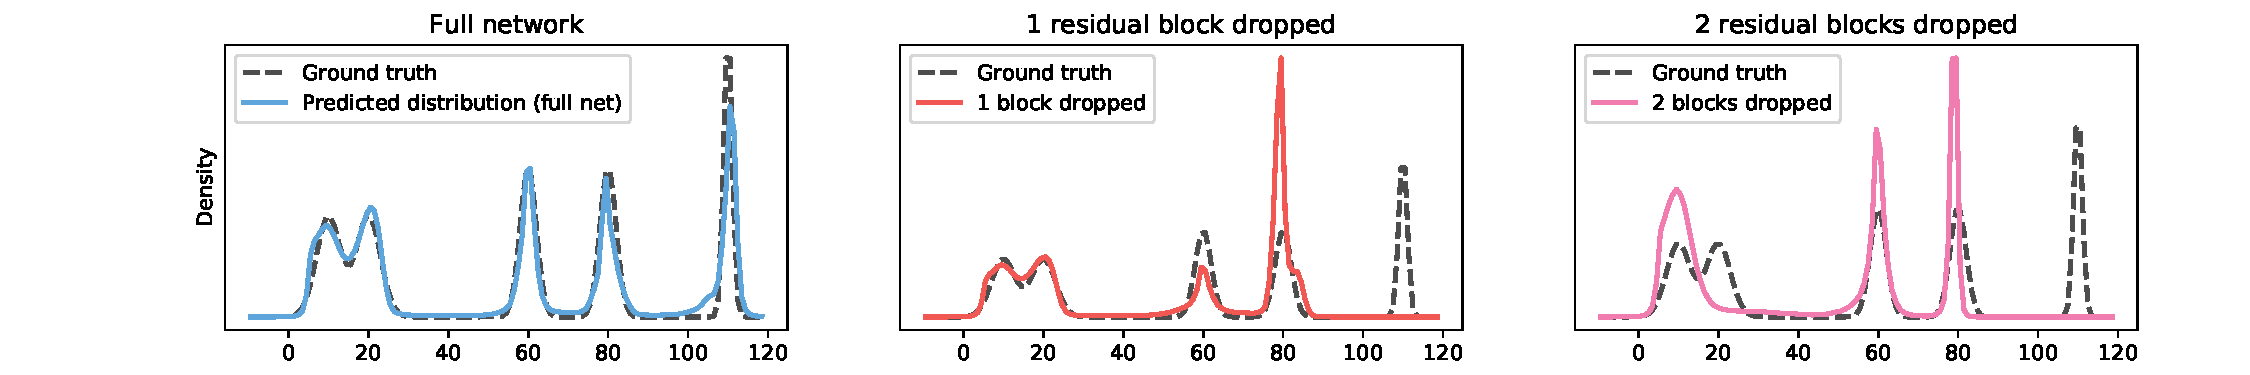
\includegraphics[width=\linewidth]{paper_images/mog.pdf}
    \caption{{\bf Block-Wise Gating:} We observe that the technique extends to not only the shapes it was trained on but can also generate images for some input shapes corresponding to other classes and to the extreme can generate images for certain shapes it never encountered during training such as the triangle and heart were directly downloaded from the internet. }
    \label{fig:block_shapes}
    \vspace{-3mm}
\end{figure*}

As evident from \figref{fig:channel_shapes}, \figref{fig:block_shapes} the gated generative techniques extend to shapes it never was shown while training. 

\section{Subset of Comparison of Results:}

We show the results of our various gating mechanisms along with all the baselines reported in the paper on the Scribble Dataset's subset of test images. These images were the ones used for Amazon Mechanical Turk and the evaluation metrics reported in the paper.
\href{http://www.robots.ox.ac.uk/~arnabg/all_results_supplementary/index.html}{Comparison of our technique vs all baselines}

\section{Distribution of Alphas:}
The histogram of the distribution of the various alphas for the block-wise setting and the channel-wise setting are shown in \figref{fig:alpha_hist}. Even without a sparsity constraint the alphas are pushed nearer the extremes rather than clustering near intermediate values. The effect is more starkly demonstrated in the case of the block wise gating, with the channel wise gating parameters being more evenly distributed.
\begin{figure*}[t]
    \centering
    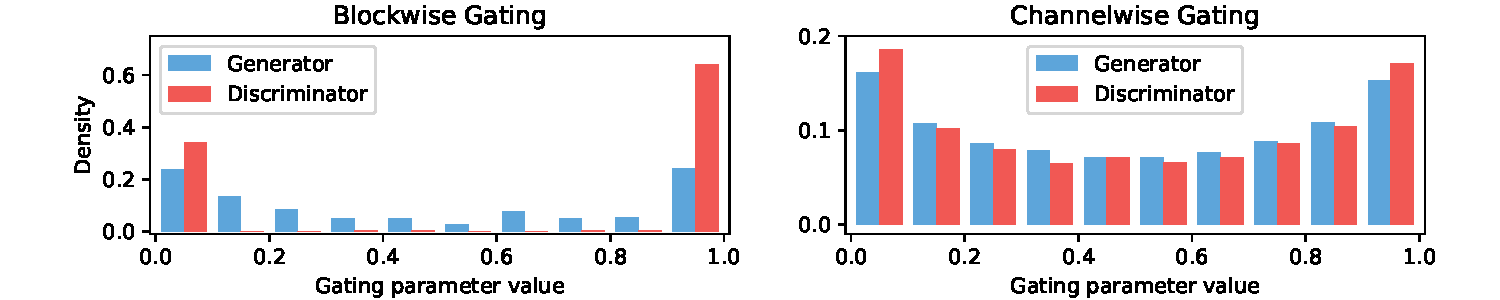
\includegraphics[width=\linewidth]{alpha_hist.pdf}
    % 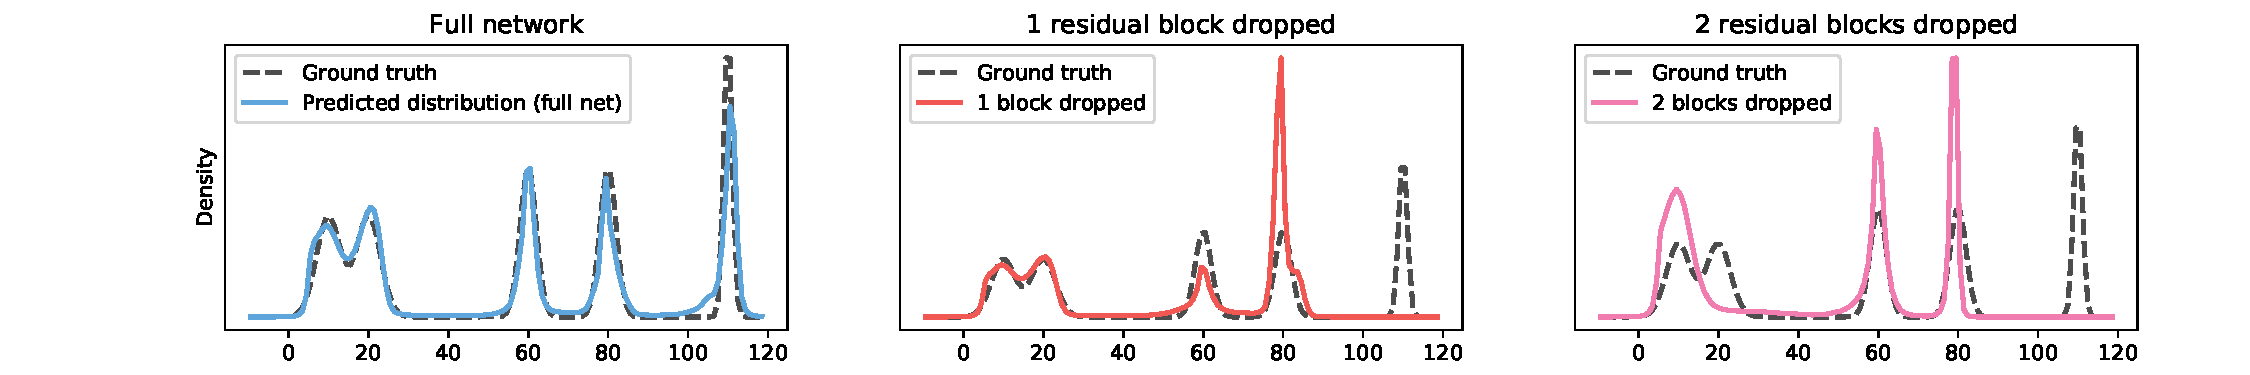
\includegraphics[width=\linewidth]{paper_images/mog.pdf}
    \caption{As we see from the distribution of the various alphas they are closer to the extremes (0 or 1) rather than the intermediate values, quite similar in the case of the channel wise gating as well }
    \label{fig:alpha_hist}
    \vspace{-3mm}
\end{figure*}

\section{Interpolations:}
In order to judge the robustness of the trained models and to analyze the differences between the naive concatenation techniques compared with our gating mechanisms we conduct some inter-class interpolations. As we can see from \figref{fig:inter_watermelon_cookie}, \figref{fig:inter_orange_basketball}, \figref{fig:inter_cookie_moon} and \figref{fig:inter_orange_cupcake} that our gating mechanisms produce smooth transitions between classes while the case of naive concatenation techniques failing to generate basketball at all, thus failing at interpolating between basketball and orange.


{\small
\bibliographystyle{ieee}
\bibliography{src/gatedblocks}
}

\begin{figure*}[t]
    \centering
    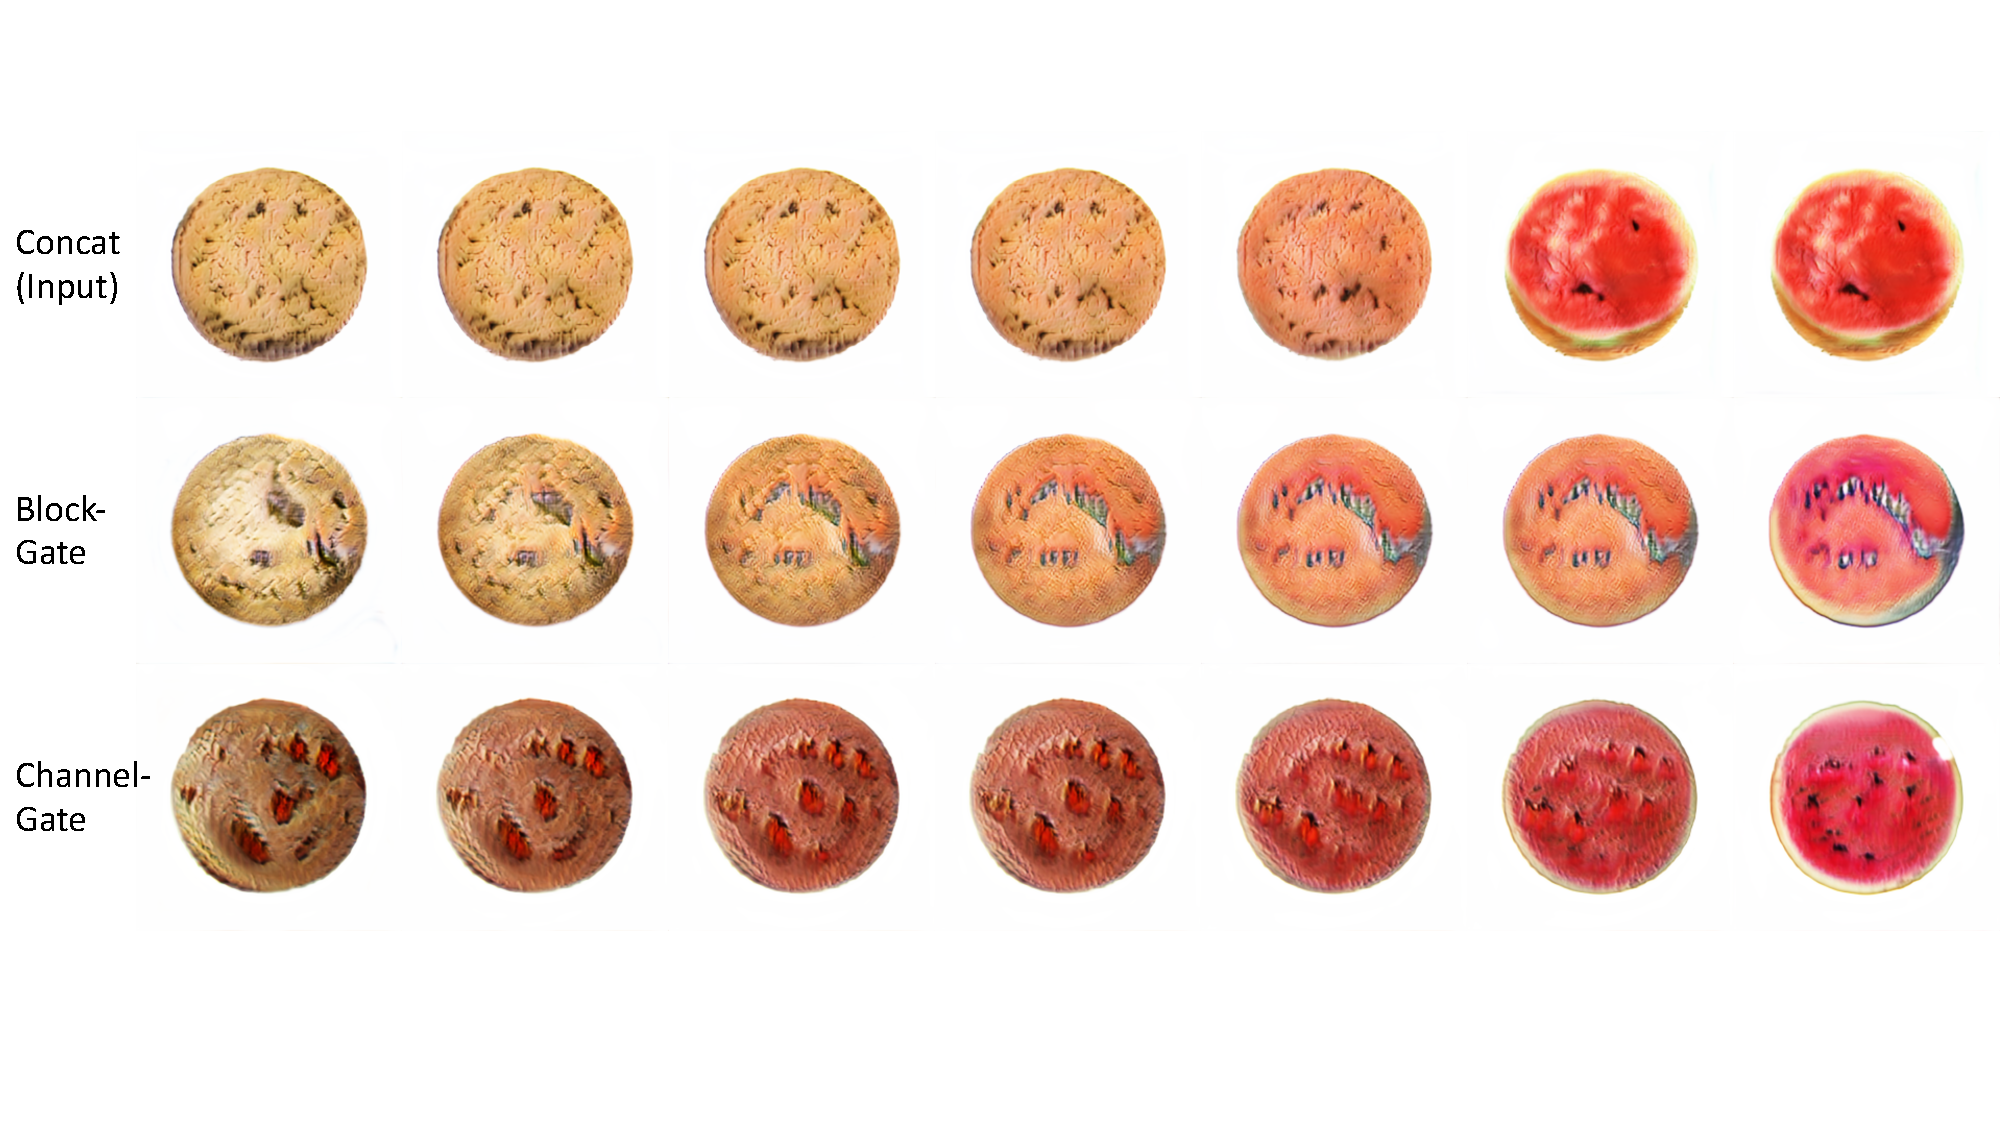
\includegraphics[width=\linewidth]{interpolation-watermelon-cookie.pdf}
    % 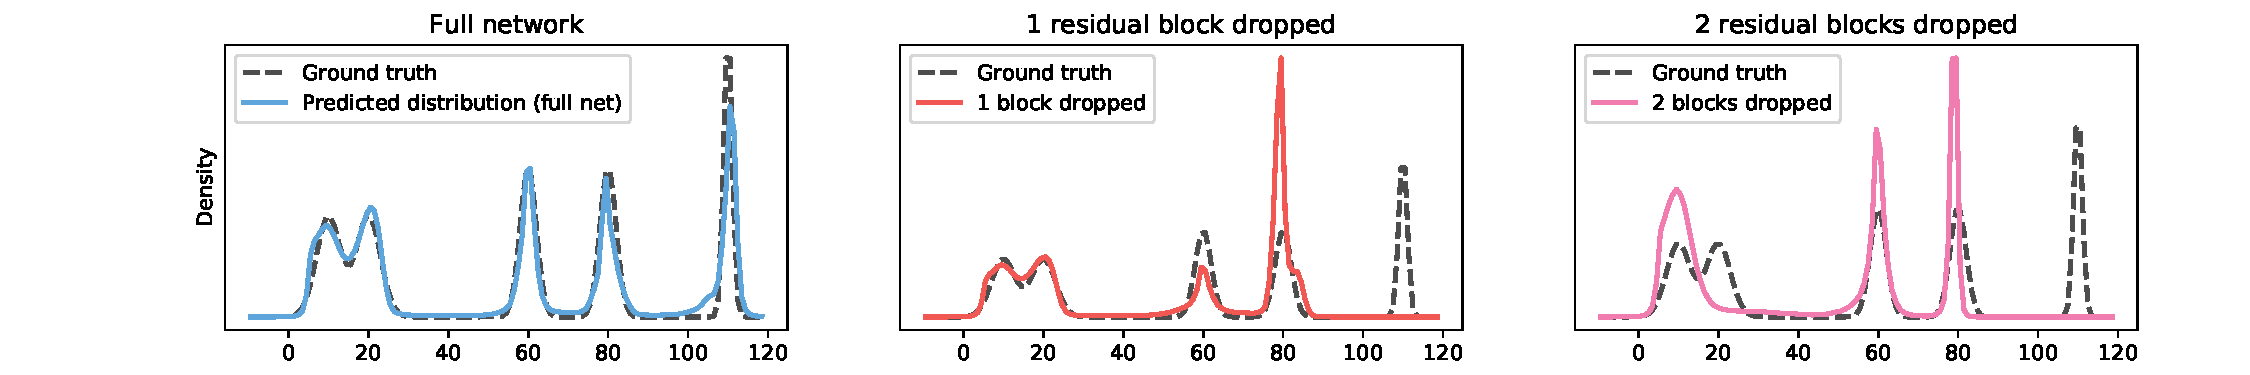
\includegraphics[width=\linewidth]{paper_images/mog.pdf}
    \caption{{\bf Cookie $\rightarrow$ Watermelon:} As evident from the interpolation the gating produces much smoother transitions than simple concatenation techniques }
    \label{fig:inter_watermelon_cookie}
    \vspace{-3mm}
\end{figure*}


\begin{figure*}[t]
    \centering
    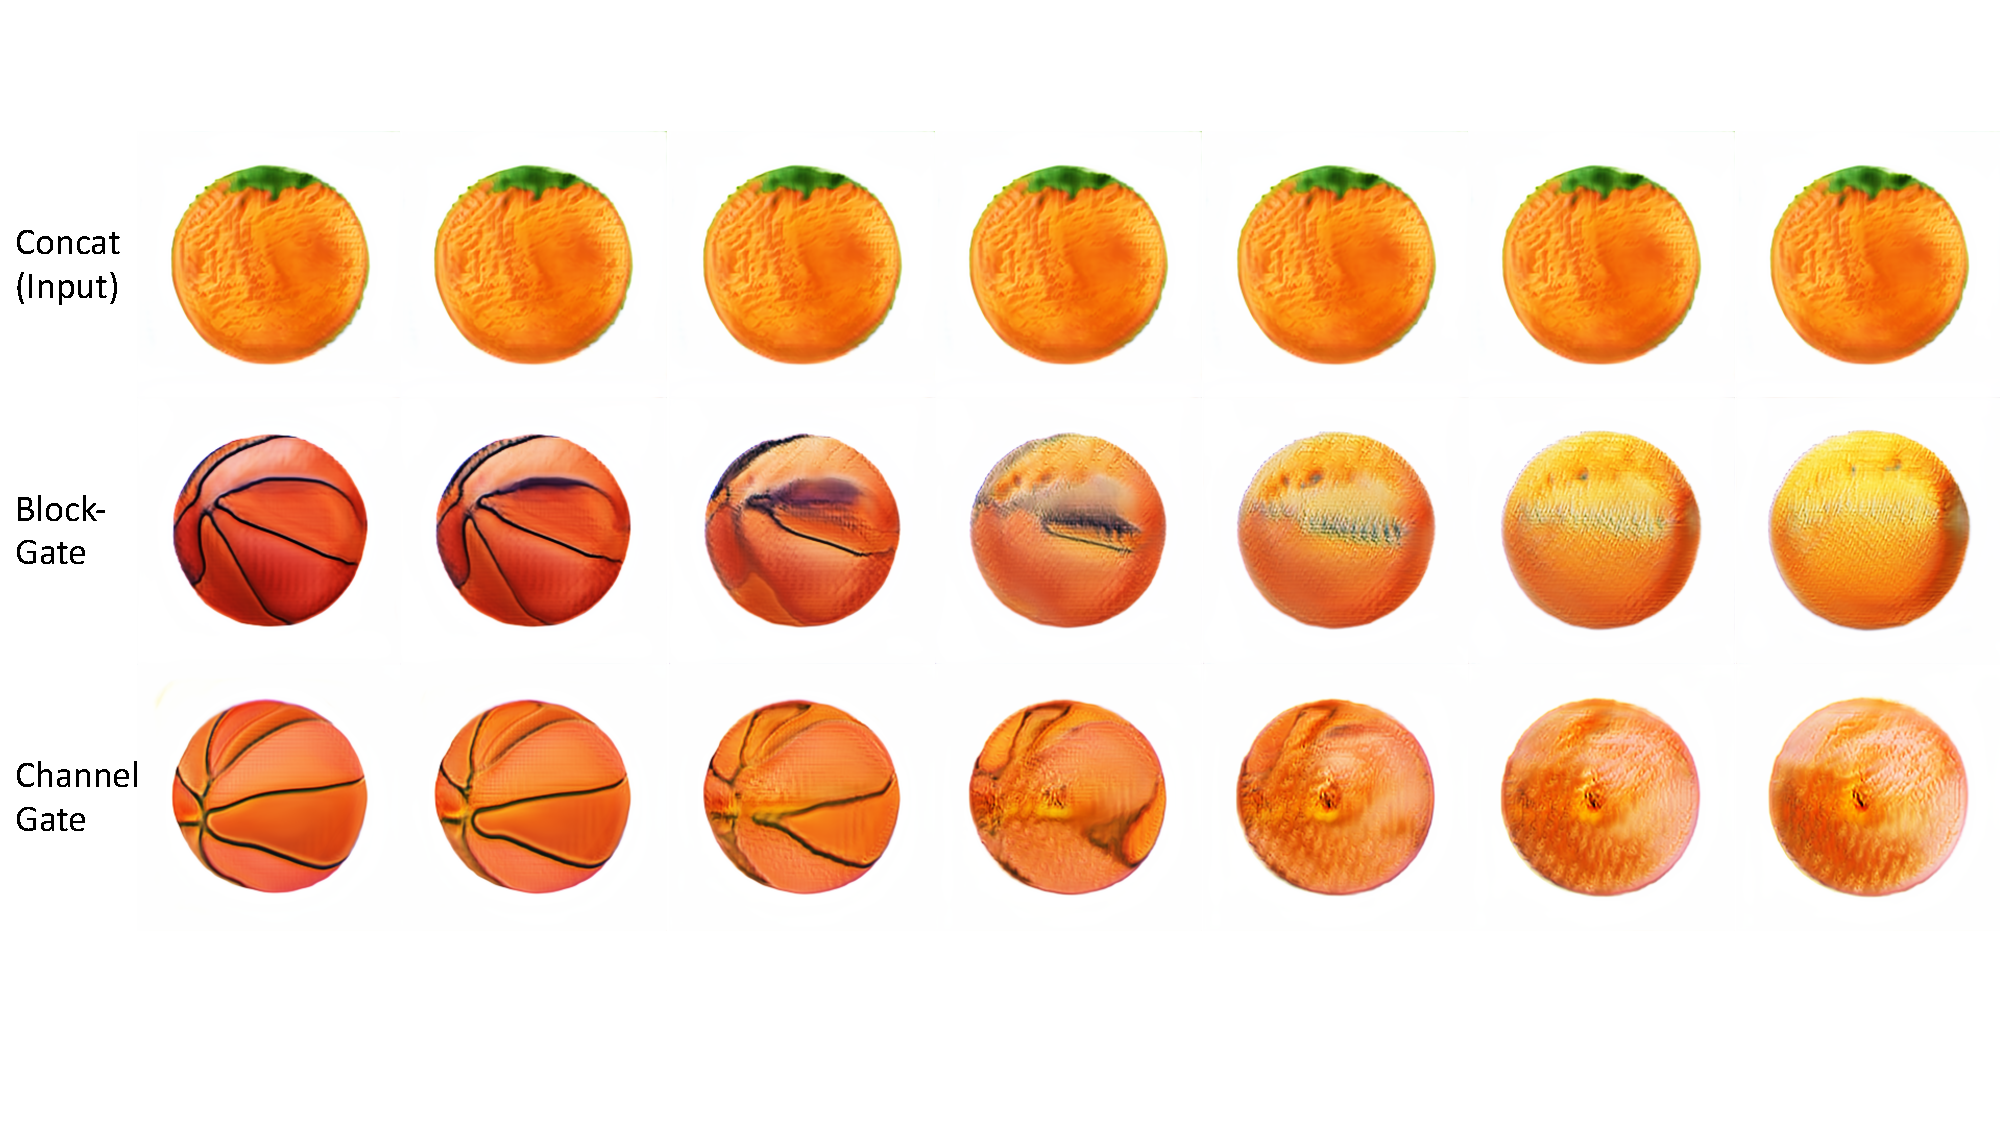
\includegraphics[width=\linewidth]{interpolation-orange-basketball.pdf}
    % 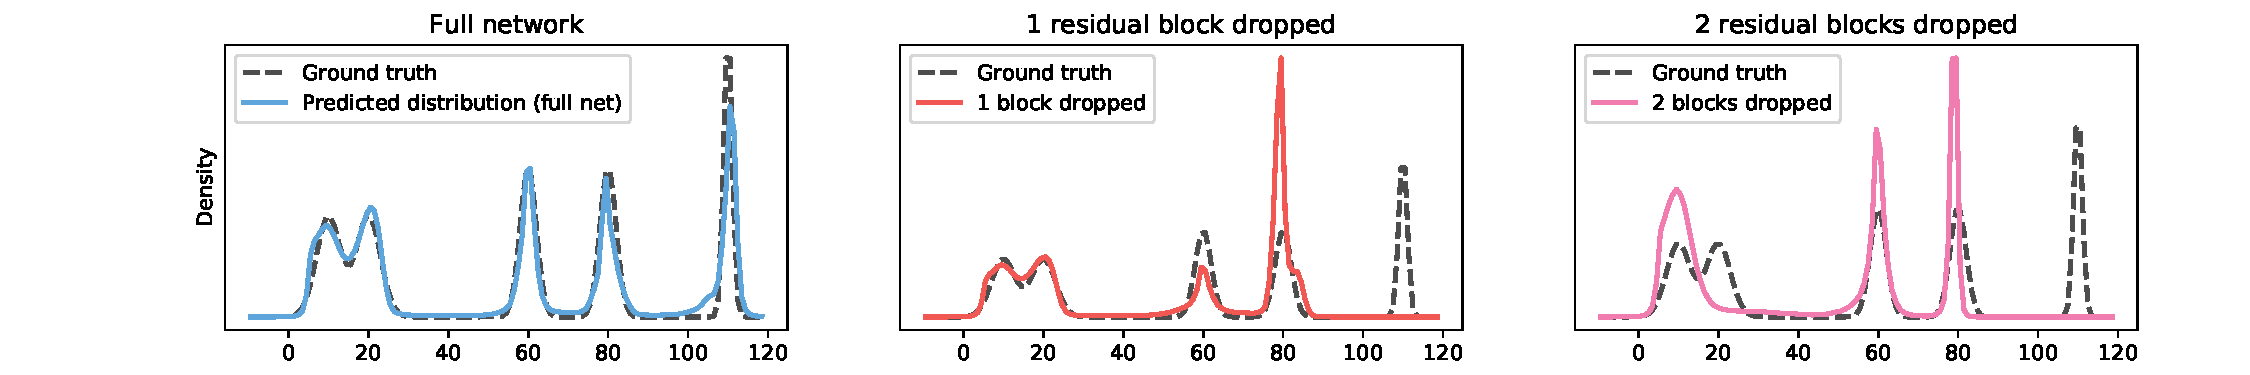
\includegraphics[width=\linewidth]{paper_images/mog.pdf}
    \caption{ {\bf Basketball $\rightarrow$ Orange:} A failure case of the simple conditioning technique, it never generates basketball and hence is not able to interpolate between basketball and orange. }
    \label{fig:inter_orange_basketball}
    \vspace{-3mm}
\end{figure*}

\begin{figure*}[t]
    \centering
    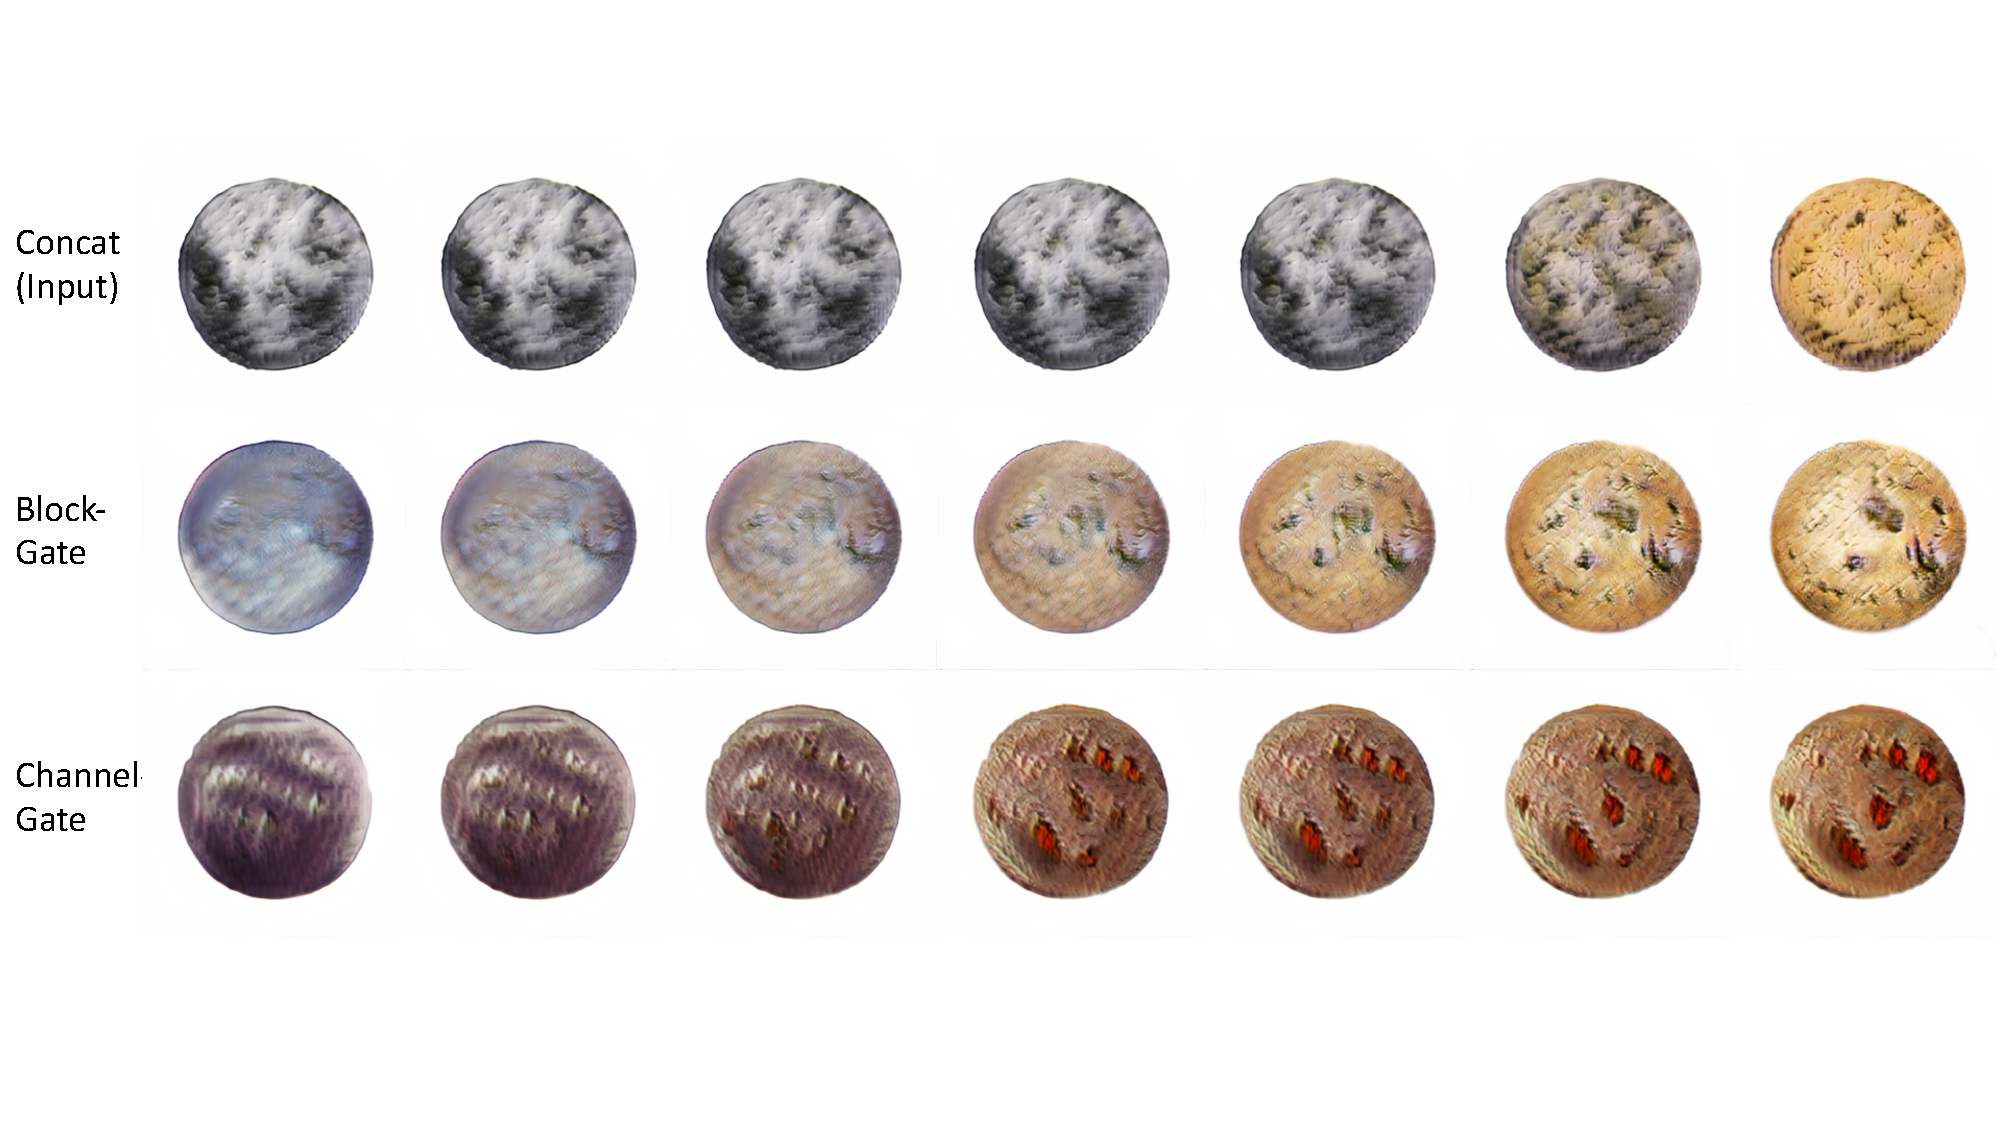
\includegraphics[width=\linewidth]{interpolation-cookie-moon.pdf}
    % 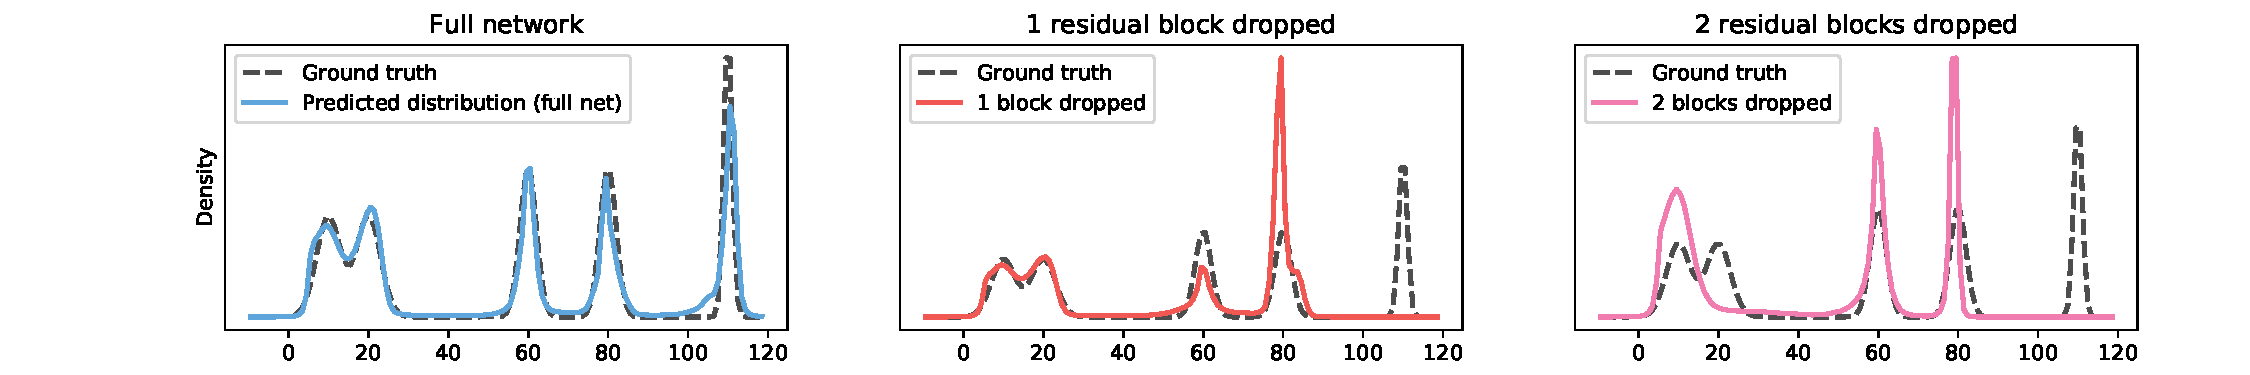
\includegraphics[width=\linewidth]{paper_images/mog.pdf}
    \caption{ {\bf Moon $\rightarrow$ Cookie:} Interpolation between moon and cookie }
    \label{fig:inter_cookie_moon}
    \vspace{-3mm}
\end{figure*}

\begin{figure*}[t]
    \centering
    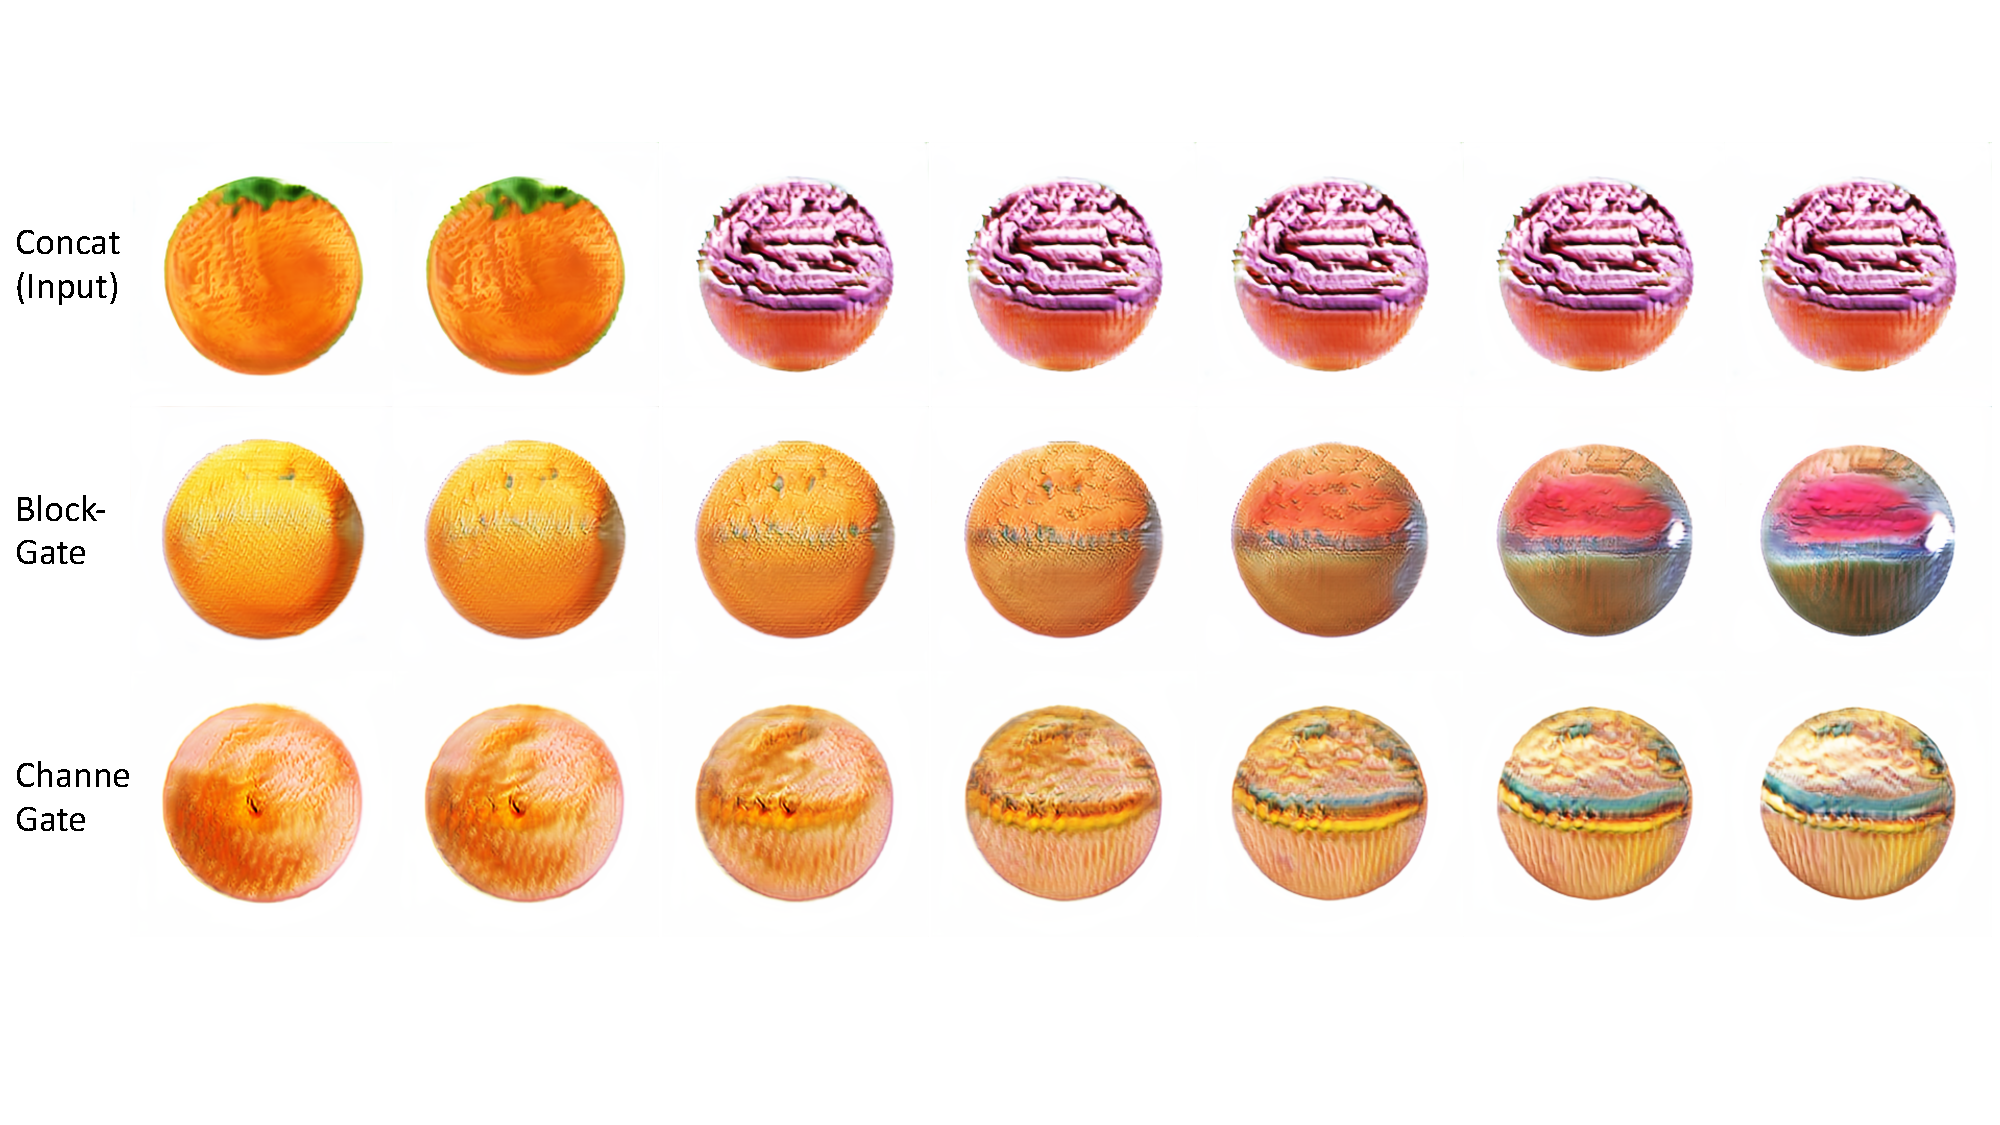
\includegraphics[width=\linewidth]{interpolation-orange-cupcake.pdf}
    % 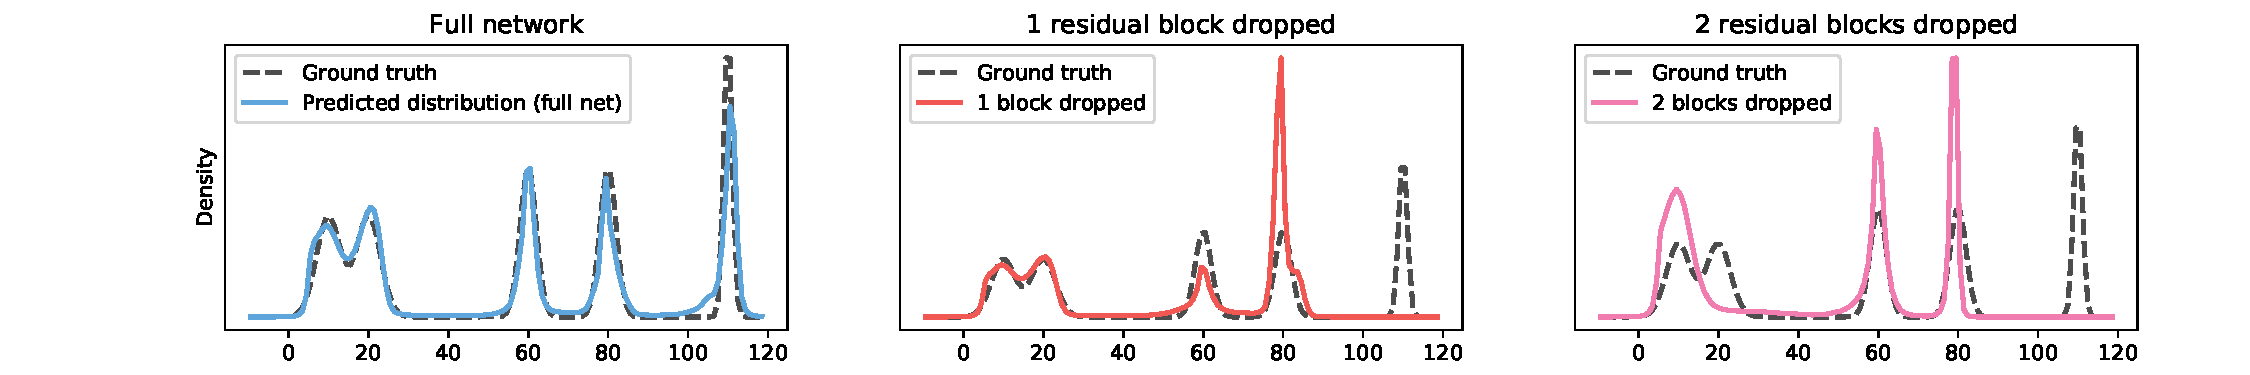
\includegraphics[width=\linewidth]{paper_images/mog.pdf}
    \caption{ {\bf Orange $\rightarrow$ Cupcake:} Interpolation between orange and cupcake, in the case of the baseline concat mechanism there's an abrupt transition from orange to cupcake while the transition is much smoother in the case of gated mechanisms }
    \label{fig:inter_orange_cupcake}
    \vspace{-3mm}
\end{figure*}




\begin{figure*}[t]
\centering
\begin{tabular}{*{2}{c@{\hspace{3px}}}}
% \textbf{Blockwise Gating} & \textbf{Channelwise Gating} \vspace{-1mm} \\
% \includegraphics[height=3.35cm,trim={0 0 0 .4cm}, clip]{paper_images/alphas_chan_1.pdf} & 
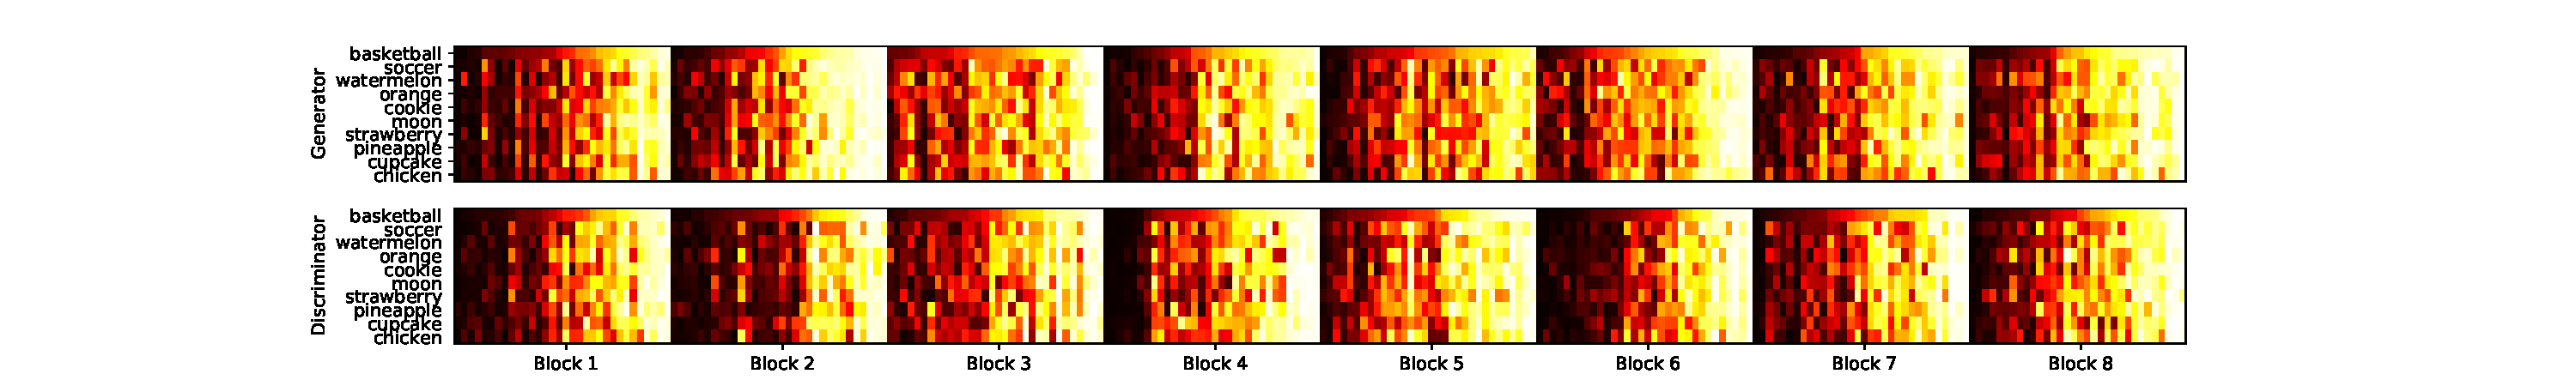
\includegraphics[height=3.15cm,trim={6.0cm 0 7.6cm .4cm}, clip]{paper_images/alphas_chan_0.pdf} & 
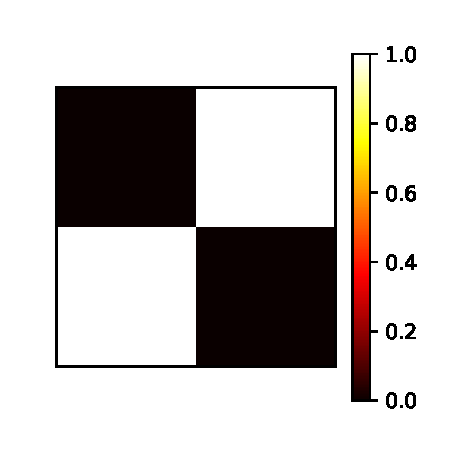
\includegraphics[height=3.15cm,trim={5.8cm 0 .2cm .4cm}, clip]{paper_images/alpha_legend.pdf}
\\
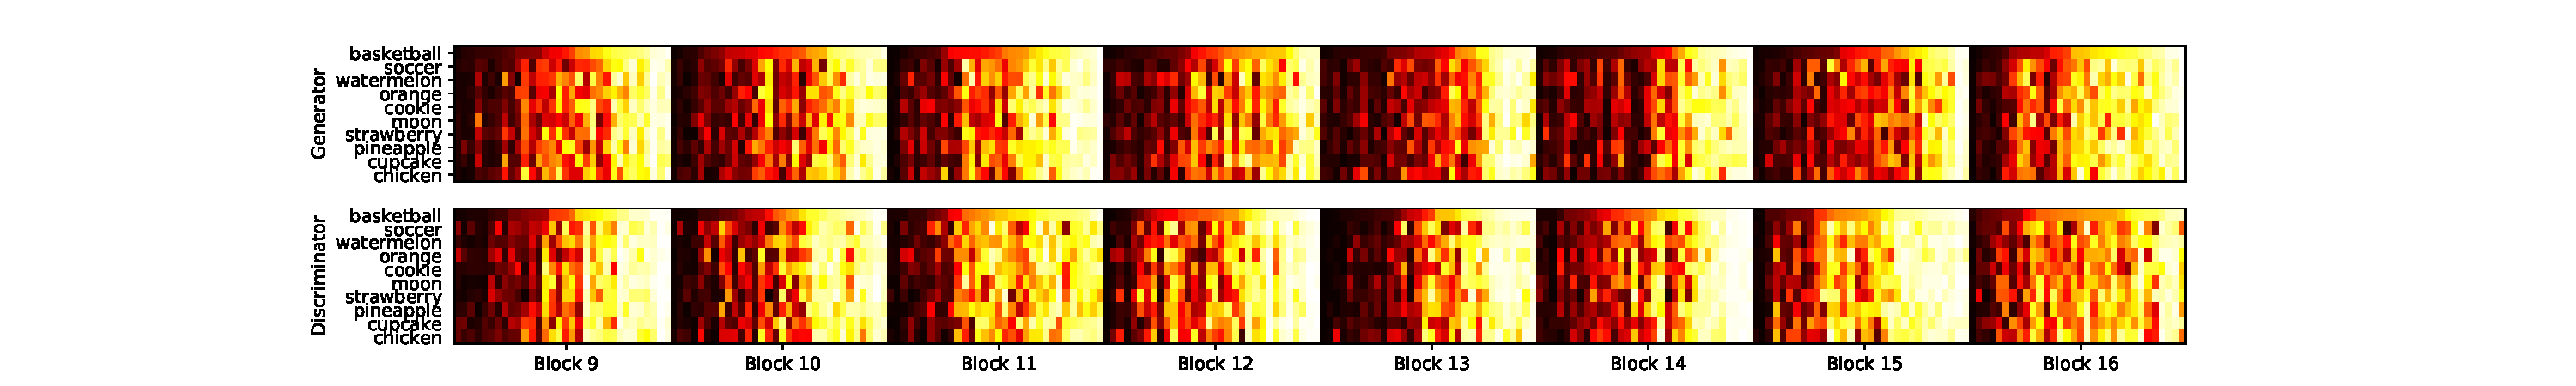
\includegraphics[height=3.15cm,trim={6.0cm 0 7.6cm .4cm}, clip]{paper_images/alphas_chan_8.pdf} & 
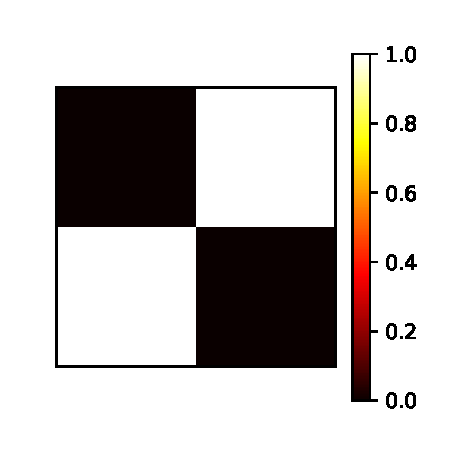
\includegraphics[height=3.15cm,trim={5.8cm 0 .2cm .4cm}, clip]{paper_images/alpha_legend.pdf}
\\
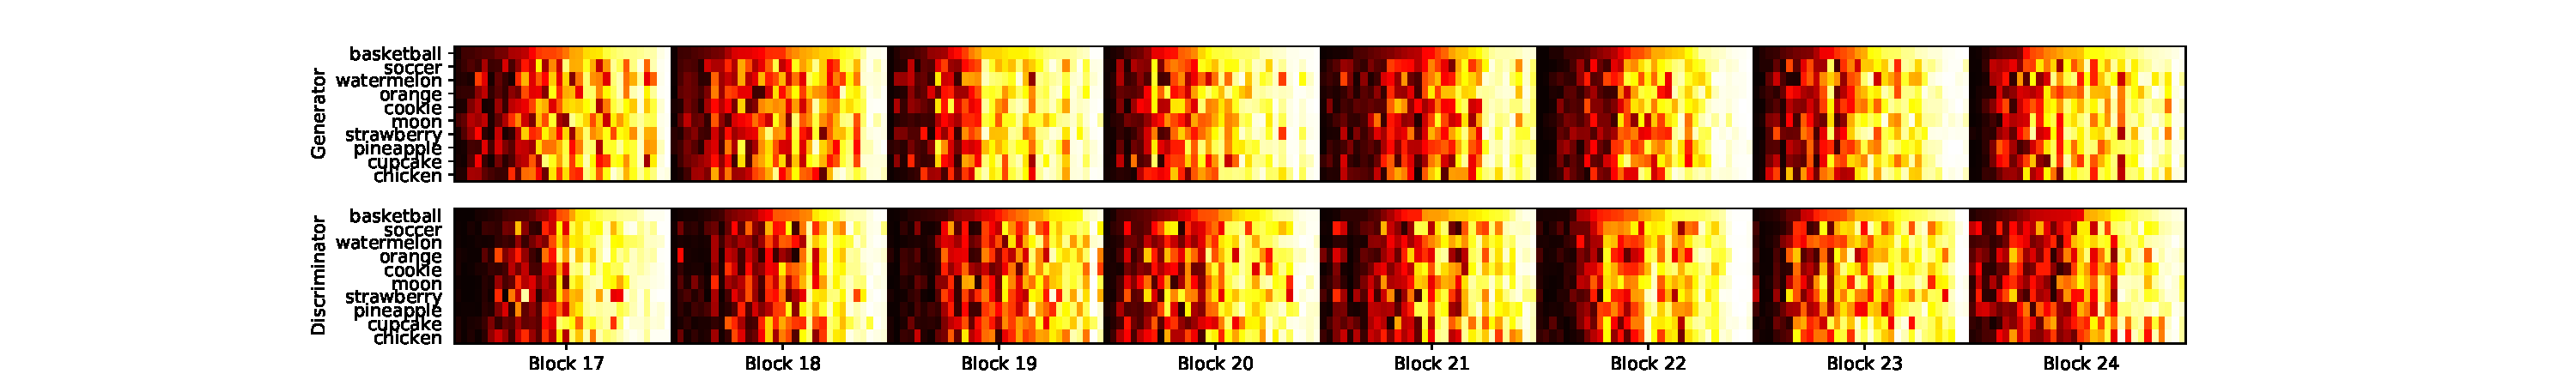
\includegraphics[height=3.15cm,trim={6.0cm 0 7.6cm .4cm}, clip]{paper_images/alphas_chan_16.pdf} & 
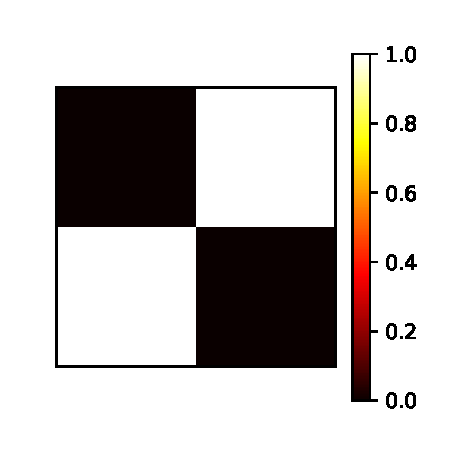
\includegraphics[height=3.15cm,trim={5.8cm 0 .2cm .4cm}, clip]{paper_images/alpha_legend.pdf}
\\

\end{tabular}
\vspace{-2mm}
\caption{\label{fig:alpha_heat}
\textbf{Learned channel-wise gating parameters.} We show the soft-gating parameters for channelwise gating for the {\bf (top)} generator and {\bf (bot)} discriminator. Black indicates
% $\alpha=0$, or
completely off, and white indicates
% $\alpha=1$, or 
completely on. We show all 24 blocks. This is an extension of Fig. 6 in the main paper. The nonuniformity of each columns indicates that different channels are used more heavily for different classes.
\vspace{-3mm}
}
\vspace{-2mm}
\end{figure*}


\begin{figure*}[h]
    \centering
    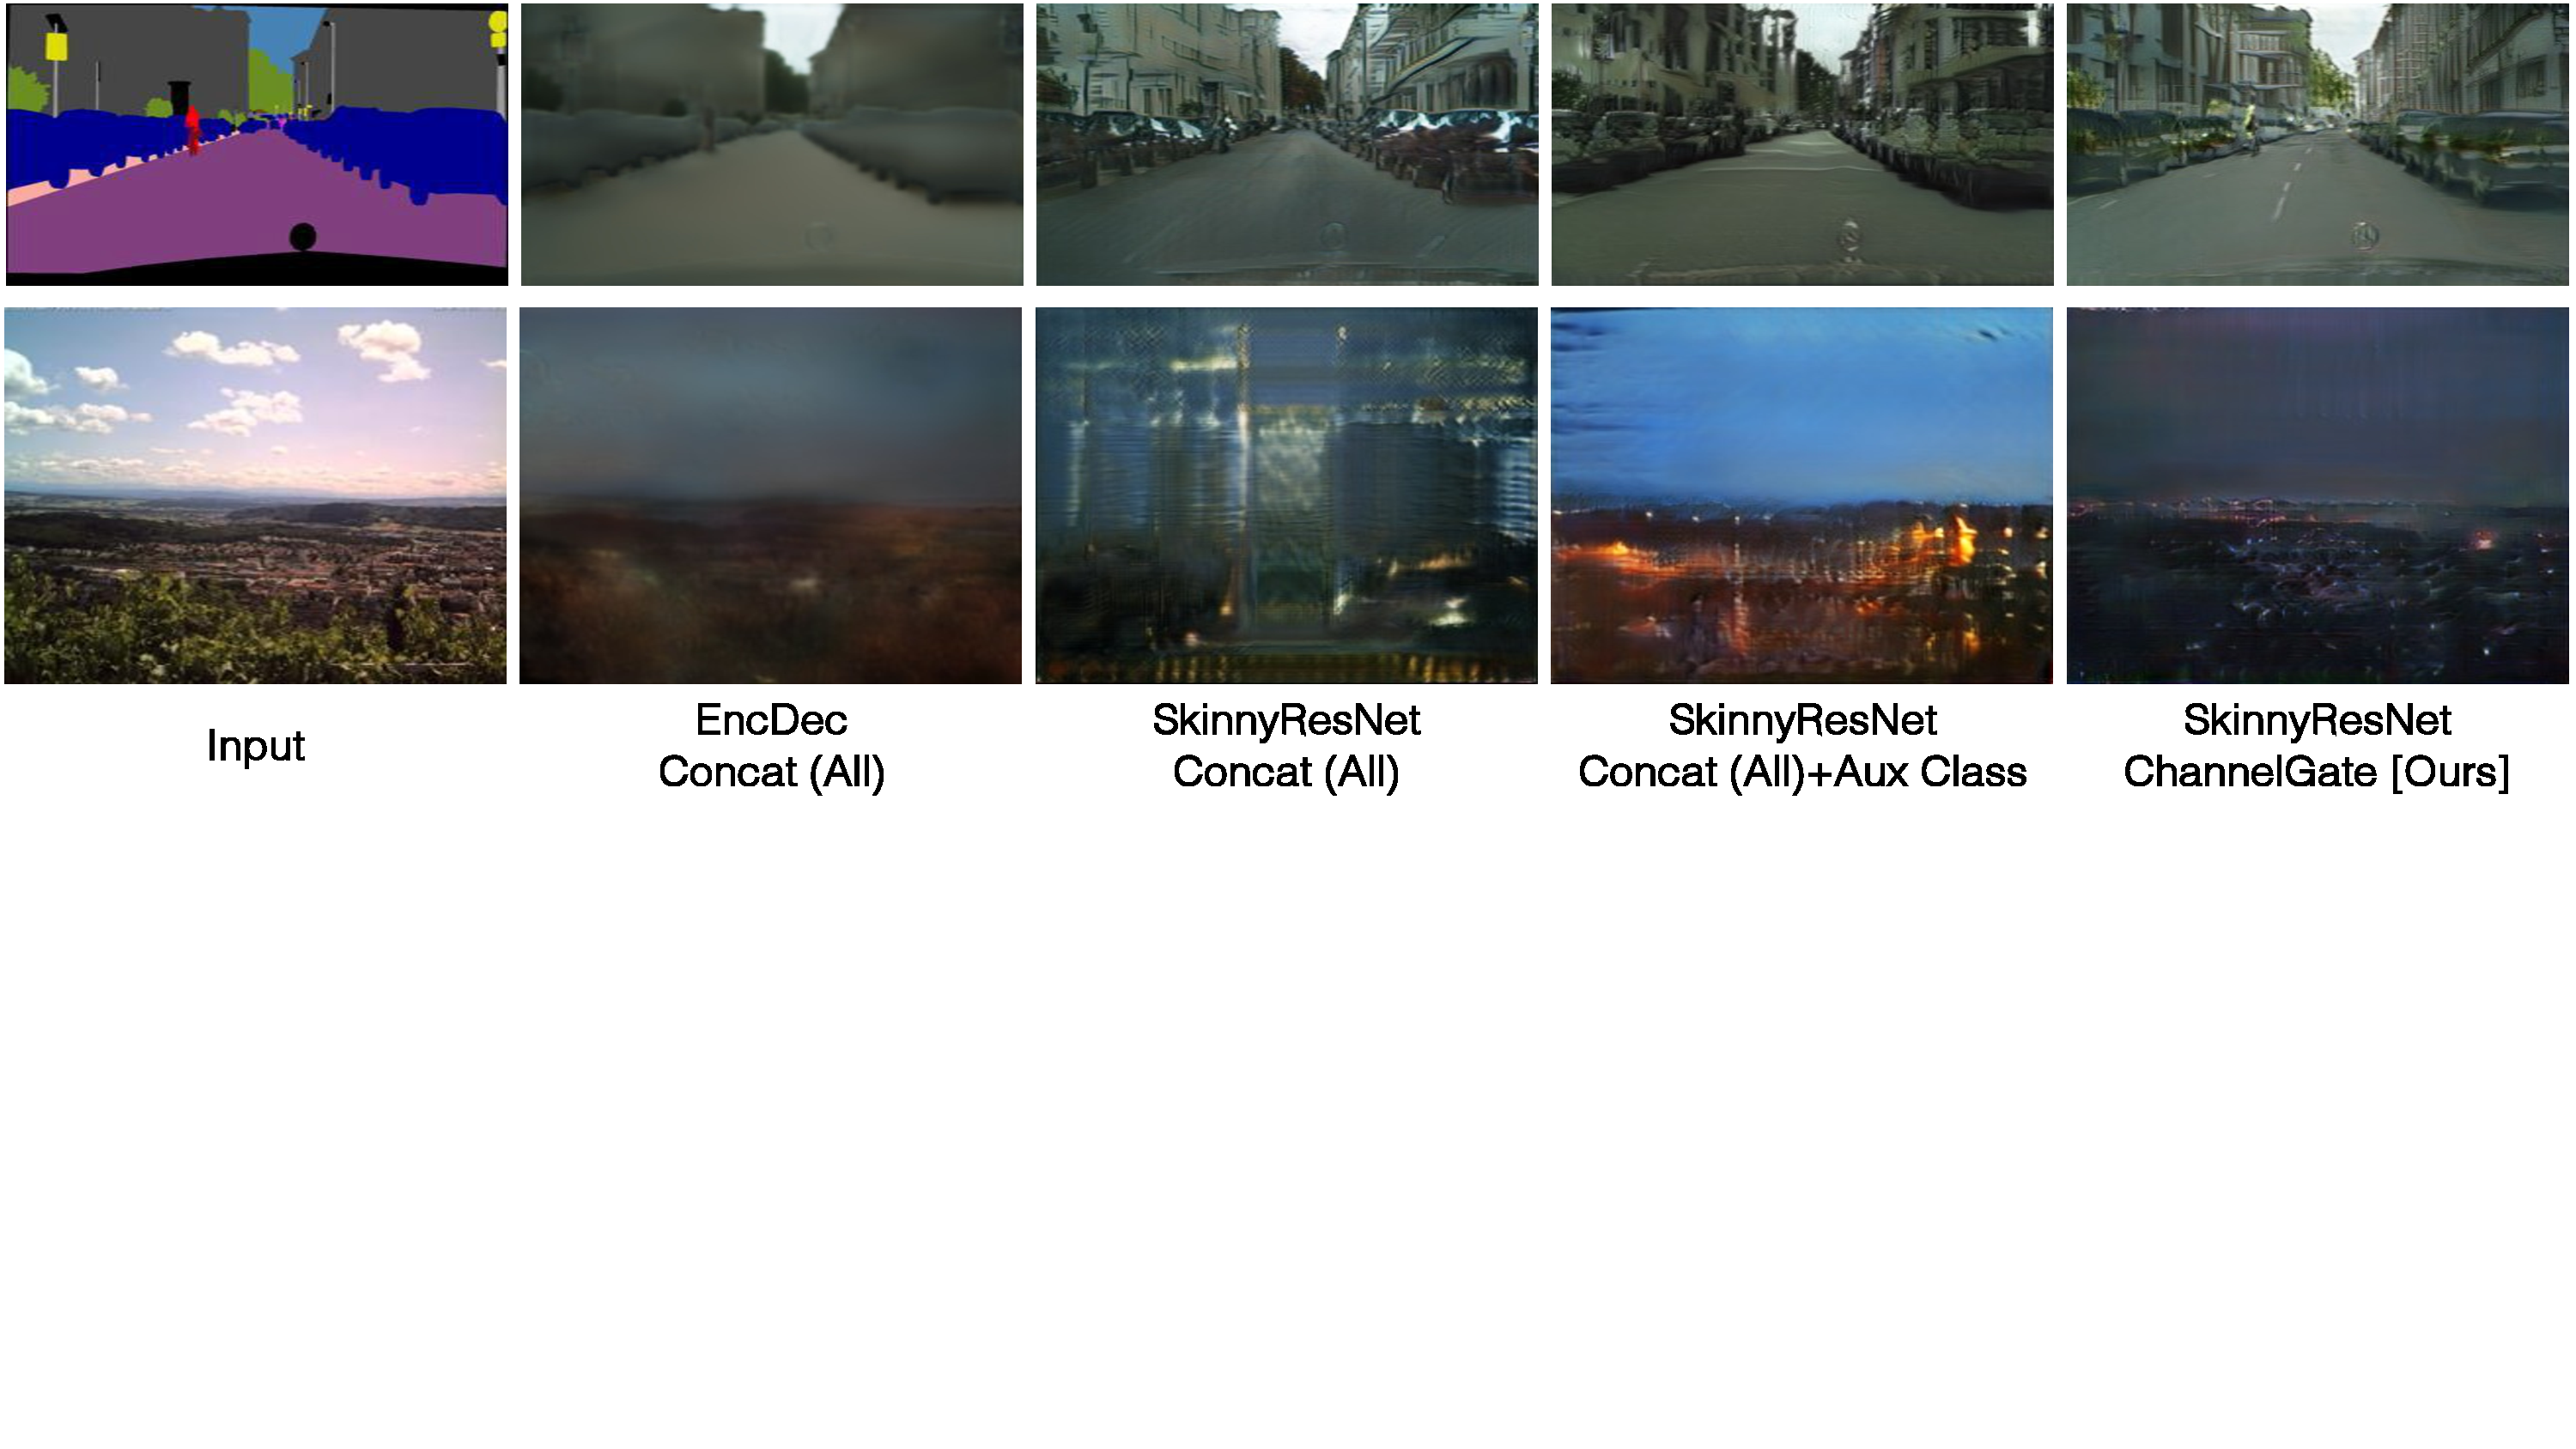
\includegraphics[width=1.\linewidth]{paper_images/multitask_comp.pdf}
    \caption{\textbf{Multitask generation results}. A single network trained on both Cityscapes Label$\rightarrow$Image and Day$\rightarrow$Night. The proposed channelwise gating method (right) is able to better incorporate task conditioning and produces more realistic results.
    % \ow{seems like this is missing 1. two generators, and 2. one generator. instead it seems more like an ablation study on our method, which is not the point. would be more impressive to show it matches 2 generators and 1 generator totally fails.}
    }
    \label{fig:multi-task_day2night}
    \vspace{-2mm}
\end{figure*}

% \documentclass[10pt,twocolumn,letterpaper]{article}

\usepackage{iccv}
\usepackage{times}
\usepackage{epsfig}
\usepackage{graphicx}
\usepackage{amsmath}
\usepackage{amssymb}
\usepackage{dsfont}
\usepackage{enumitem}
\usepackage{multicol}
\usepackage{multirow}
\usepackage{amsbsy}
\usepackage{array, floatrow, tabularx, makecell, booktabs}%

%%%%%%%%%%%%%%
% Packages and stuff custom
%%%%%%%%%%%%%%
\usepackage{url}
\usepackage{amsthm}
\usepackage{color}
\usepackage{subcaption}
\captionsetup{compatibility=false}
\usepackage{booktabs}
\usepackage{arydshln}
%\usepackage{hyperref}
% If you comment hyperref and then uncomment it, you should delete
% egpaper.aux before re-running latex.  (Or just hit 'q' on the first latex
% run, let it finish, and you should be clear).
\usepackage[pagebackref=true,breaklinks=true,letterpaper=true,colorlinks,bookmarks=false]{hyperref}

\DeclareMathOperator{\E}{\mathbb{E}}
\DeclareMathOperator{\R}{\mathbb{R}}

\def\figref#1{Fig.~\ref{#1}}
\def\secref#1{\S\ref{#1}}
\def\tabref#1{Table~\ref{#1}}
\def\eqnref#1{Eq.~\ref{#1}}

\newcommand{\ow}[1]{\textbf{\textcolor[rgb]{.1, .1, .8}{OW: #1}}}
\newcommand{\rz}[1]{\textbf{\textcolor[rgb]{.54, .16, .55}{RZ: #1}}}
\newcommand{\todo}[1]{\textbf{\textcolor[rgb]{.8, .1, .1}{#1}}}
\newcommand{\pd}[1]{\textbf{\textcolor[rgb]{1, 0.5, 0}{PD: #1}}}
\newcommand{\eli}[1]{\textbf{\textcolor[rgb]{0.1, 0.6, 0.1}{ES: #1}}}
\newcommand{\ag}[1]{\textbf{\textcolor[rgb]{0.45, 0.25, 0.1}{AG: #1}}}

%% spacehacks
%\setlength{\abovecaptionskip}{-5pt}


\newcommand{\addSubFigHalf}[3]{\begin{subfigure}[t]{.45\linewidth}
   \includegraphics[width=\linewidth]{#1}
   \caption{#2}\label{#3}\end{subfigure}
}
\newcommand{\addSubFigThird}[3]{\begin{subfigure}[t]{.31\linewidth}
   \includegraphics[width=\linewidth]{#1}
   \caption{#2}\label{#3}\end{subfigure}
}
\newcommand{\addSubFigTenth}[3]{\begin{subfigure}[t]{.16\linewidth}
   \includegraphics[width=\linewidth]{#1}
   \caption{#2}\label{#3}\end{subfigure}
}
\newcommand{\addSubFigSixth}[2]{\begin{subfigure}[t]{.12\linewidth}
   \includegraphics[width=\linewidth]{#1}
   \label{#2}\end{subfigure}
}
\newcommand{\addSubFigSixthLabel}[3]{\begin{subfigure}[t]{.12\linewidth}
   %\rotatebox{90}{#2}
   \includegraphics[width=.9\linewidth]{#1}
   \caption{#2}\label{#3}\end{subfigure}
}



\newcommand{\model}[0]{GateGAN}

\DeclareGraphicsExtensions{.pdf,.jpg}

%%%%%%%%%%%%%%%

\graphicspath{ {images/}{syntheticExp/} {final_images/channel_gated/} {final_images/} {paper_images/} }
%%%%%%%%%%%%%%%%


% Include other packages here, before hyperref.

% If you comment hyperref and then uncomment it, you should delete
% egpaper.aux before re-running latex.  (Or just hit 'q' on the first latex
% run, let it finish, and you should be clear).
\usepackage[pagebackref=true,breaklinks=true,letterpaper=true,colorlinks,bookmarks=false]{hyperref}

% \cvprfinalcopy % *** Uncomment this line for the final submission

\def\iccvPaperID{4121} % *** Enter the CVPR Paper ID here
\def\httilde{\mbox{\tt\raisebox{-.5ex}{\symbol{126}}}}

% Pages are numbered in submission mode, and unnumbered in camera-ready
\ificcvfinal\pagestyle{empty}\fi
\begin{document}

%%%%%%%%% TITLE
\title{Interactive Sketch \& Fill: Multiclass Sketch-to-Image Translation \\ Supplementary Material}
% \title{GAN-Gate: Gated Residual GANs for Class-Conditioned Image Generation}
% GAN-Gate: Softly-Gated Conditional Residual Networks for Image-to-Image Translation
% GAN-Gate: Conditionally Soft-Gated Residual Networks for Image-to-Image Translation
%GAN-Gate: Conditional Gating for Image-to-Image Translation

\author{Arnab Ghosh\\
University of Oxford\\
{\tt\small arnab.ghosh@eng.ox.ac.uk}
% For a paper whose authors are all at the same institution,
% omit the following lines up until the closing ``}''.
% Additional authors and addresses can be added with ``\and'',
% just like the second author.
% To save space, use either the email address or home page, not both
\and
Puneet Dokania\\
University of Oxford\\
{\tt\small puneet@robots.ox.ac.uk}
\and
Richard Zhang\\
Adobe Research\\
{\tt\small rizhang@adobe.com}
\and
Oliver Wang\\
Adobe Research\\
{\tt\small owang@adobe.com}
\and
Philip Torr\\
University of Oxford\\
{\tt\small philip.torr@eng.ox.ac.uk}
\and
Eli Shechtman\\
Adobe Research\\
{\tt\small elishe@adobe.com}
}

\maketitle


\section{User Study (User Interface):}
In order to analyze how users perceive the effects of different components of the user interface, we conducted a pilot study with 14 participants who were all graduate students of computer science in the age group of 20-30 and about 30\% of them women and 70\% men with little to no artistic experience. 
% \todo{who were all graduate students in computer science, with little to no artistic experience. (or something like that, you usually see age range/gender/where we sourced them written out here)}. 
We attempted to study three main variables: \textbf{outlines vs edges, interactivity vs no interactivity, and completion hints vs no completion hints.} 
Each participant was instructed to use each variant of our system, presented in a random order, in order to generate realistic images from 5 random classes. 
Each user was asked to rate his/her performance on the NASA Task Load Index (lower the better). \cite{hart1988development}. 


\begin{figure*}[t]
    \centering
    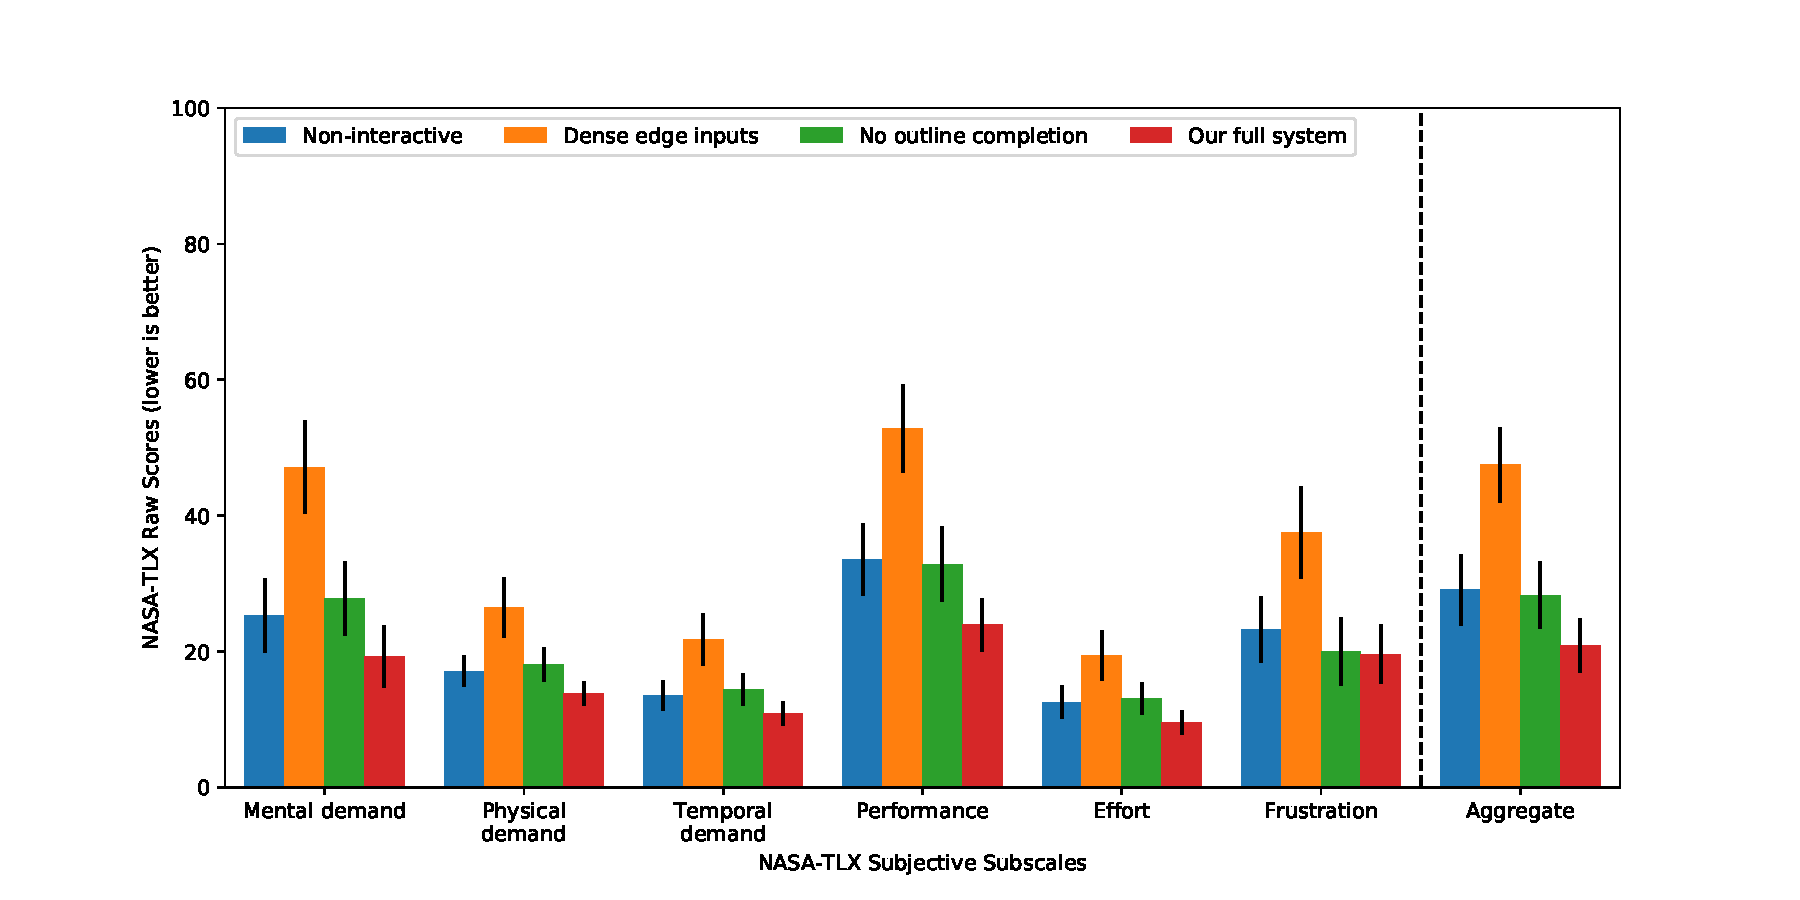
\includegraphics[width=\linewidth]{user_study/barplots.pdf}
    \caption{{\bf NASA TLX Score Comparisons (lower is better): }
    The NASA TLX Questionnaire consists of 6 different subjective scales the raw scores for the various interfaces are depicted in the figure, the aggregate is computed using the weight of each subjective subscale using a pair-wise importance ranking performed by the subject. We see that our full system systematically obtains the lowest scores in all the subjective subscales while the one with the dense edge inputs obtains the highest.\label{fig:nasa-tlx}
    \vspace{-2mm}
    }
    \vspace{-2mm}
\end{figure*}

\begin{table*}[h]
\resizebox{\linewidth}{!}{
\caption{\textbf{User Study: User Interfaces}} % title of Table
\centering % used for centering table
\begin{tabular}{l c c c c}
%  \hline
\toprule
\textbf{Interface} & \textbf{Input} & \textbf{Recommendation} &  \textbf{Interactive} & \textbf{Mean Aggregate Score} \\ \midrule
Non Interactive & Outline & \checkmark &  & 29.01\\ %\midrule
Dense Edge Inputs & Edge & \checkmark & \checkmark & 47.50 \\ 
No outline completion & Outline & & \checkmark & 28.29\\ 
\textbf{Our Full System} & \textbf{Outline} & \textbf{\checkmark} & \textbf{\checkmark} & \textbf{20.83} \\
\bottomrule %inserts single line
\end{tabular}
\label{table:user_study} % is used to refer this table in the text
}
\end{table*}

% \begin{itemize}
%     \item \textbf{A:} Backend: 2-stage, Input type: Outline, with recommendation, no interactivity
%     \item \textbf{B:} Backend: 2-stage, Input type: Edge, with recommendation, with interactivity
%     \item \textbf{C:} Backend: 2-stage, Input type: Outline, no recommendation, with interactivity 
%     \item \textbf{D:} Backend: 2-stage, Input type: Outline, with recommendation, with interactivity 
% \end{itemize}




\subsection{NASA TLX: Details}
NASA TLX questionnaire \cite{hart1988development} is a standard questionnaire used by psychological studies which gauges workload of a task on 6 metrics namely: Mental Demand, Physical Demand, Temporal Demand, Performance, Effort and Frustration. Since different people interpret these terms differently first they are provided with a pairwise comparison of each of the terms being the most important contributor to the workload for the given task. The ratings on each of these scales are weighted by the relative importance (obtained from the pairwise comparisons) and averaged out to get a score from 0-100 which represents the workload for the current task (lower is better).

\tabref{table:user_study} shows the mean aggregate scores obtained for each interface, aggregate scores are obtained by weighting each subjective score on the individual metric by the user's pairwise importance ranking. For a more detailed analysis into the individual metrics please refer to \figref{fig:nasa-tlx} which provides the raw scores (unweighted) for each individual metric.



% \begin{table}[ht]
% \caption{\textbf{User Study: User Interface} NASA TLX Index Mean \textbf{(Aggregate)} scores (lower is better)} % title of Table
% \centering % used for centering table
% \begin{tabular}{l c}
% %  \hline
% \toprule
% \textbf{Interface} & \textbf{Mean}  \\ \midrule
% Non Interactive & Outline & 29.01 \\ %\midrule
% Dense Edge Inputs & 47.50 \\ 
%  & 28.29 \\ 
% \textbf{D} & \textbf{20.83}\\
% \bottomrule %inserts single line
% \end{tabular}
% \label{table:user_study} % is used to refer this table in the text
% \end{table}

As depicted in \tabref{table:user_study} and \figref{fig:nasa-tlx} we can see that:

\begin{itemize}
    \item \textbf{Outlines vs Edges:} Mean score for Our Full System is lesser than Dense Edge Inputs thus indicating that users prefer a model trained with outlines compared to one trained with edges.
    \item \textbf{Interactivity vs No Interactivity:} Mean score for No outline completion and Our Full System which are outline based but has interactivity shows lower scores than Non Interactive which doesn't have interactivity. This shows that users prefer interactivity to non-interactivity.
    \item \textbf{Sketch Recommendation vs No Sketch Recommendation:} Mean score for Our Full System which has outline-completion based recommendation for the sketch are lower than for No outline completion thus indicating that users prefer recommended outlines over no outline recommendation.
\end{itemize}

A further larger scale study might be needed to fully validate the hypotheses. However, this pilot study shows that a recommendation system (sketch completion) where the outline completion is shown along along with the corresponding generated image, was given the highest preference by the users.



\section{Shape Completion: Details}

The Bicycle GAN model \cite{zhu2017toward} was used to train the shape completion model with minor modifications. In order for the BicycleGAN model to generate the shape completion appropriate for the correct class the class condition was concatenated to the input as a one hot encoding in the Generator, Discriminator and the Encoder. Since the class condition worked decently we didn't try introducing gating in those scenarios but it can potentially be introduced although the gating might potentially produce multimodal results. The input domain images for the model consisted of the partial versions of the sketches or outlines and the target domain for the model consisted of the completed sketches or outlines. 

The training and testing input partial sketches and partial outlines were created using the same modus operandi whereby for each sketch/outline occluders of 3 sizes (64x64,128x128,192x192) were used and for each size of occluder 25 partial sketches/outlines were created, thus creating 75 partial versions from a single sketch/outline.


\section{Appearance Generation: Details}
For more details about the various architectures described in Section 4.2 in the main paper we show the schematic representation of all the above mentioned models can be observed in \figref{fig:arch-inj} and Figure 5 in the main paper.

\begin{figure*}[t]
    \centering
    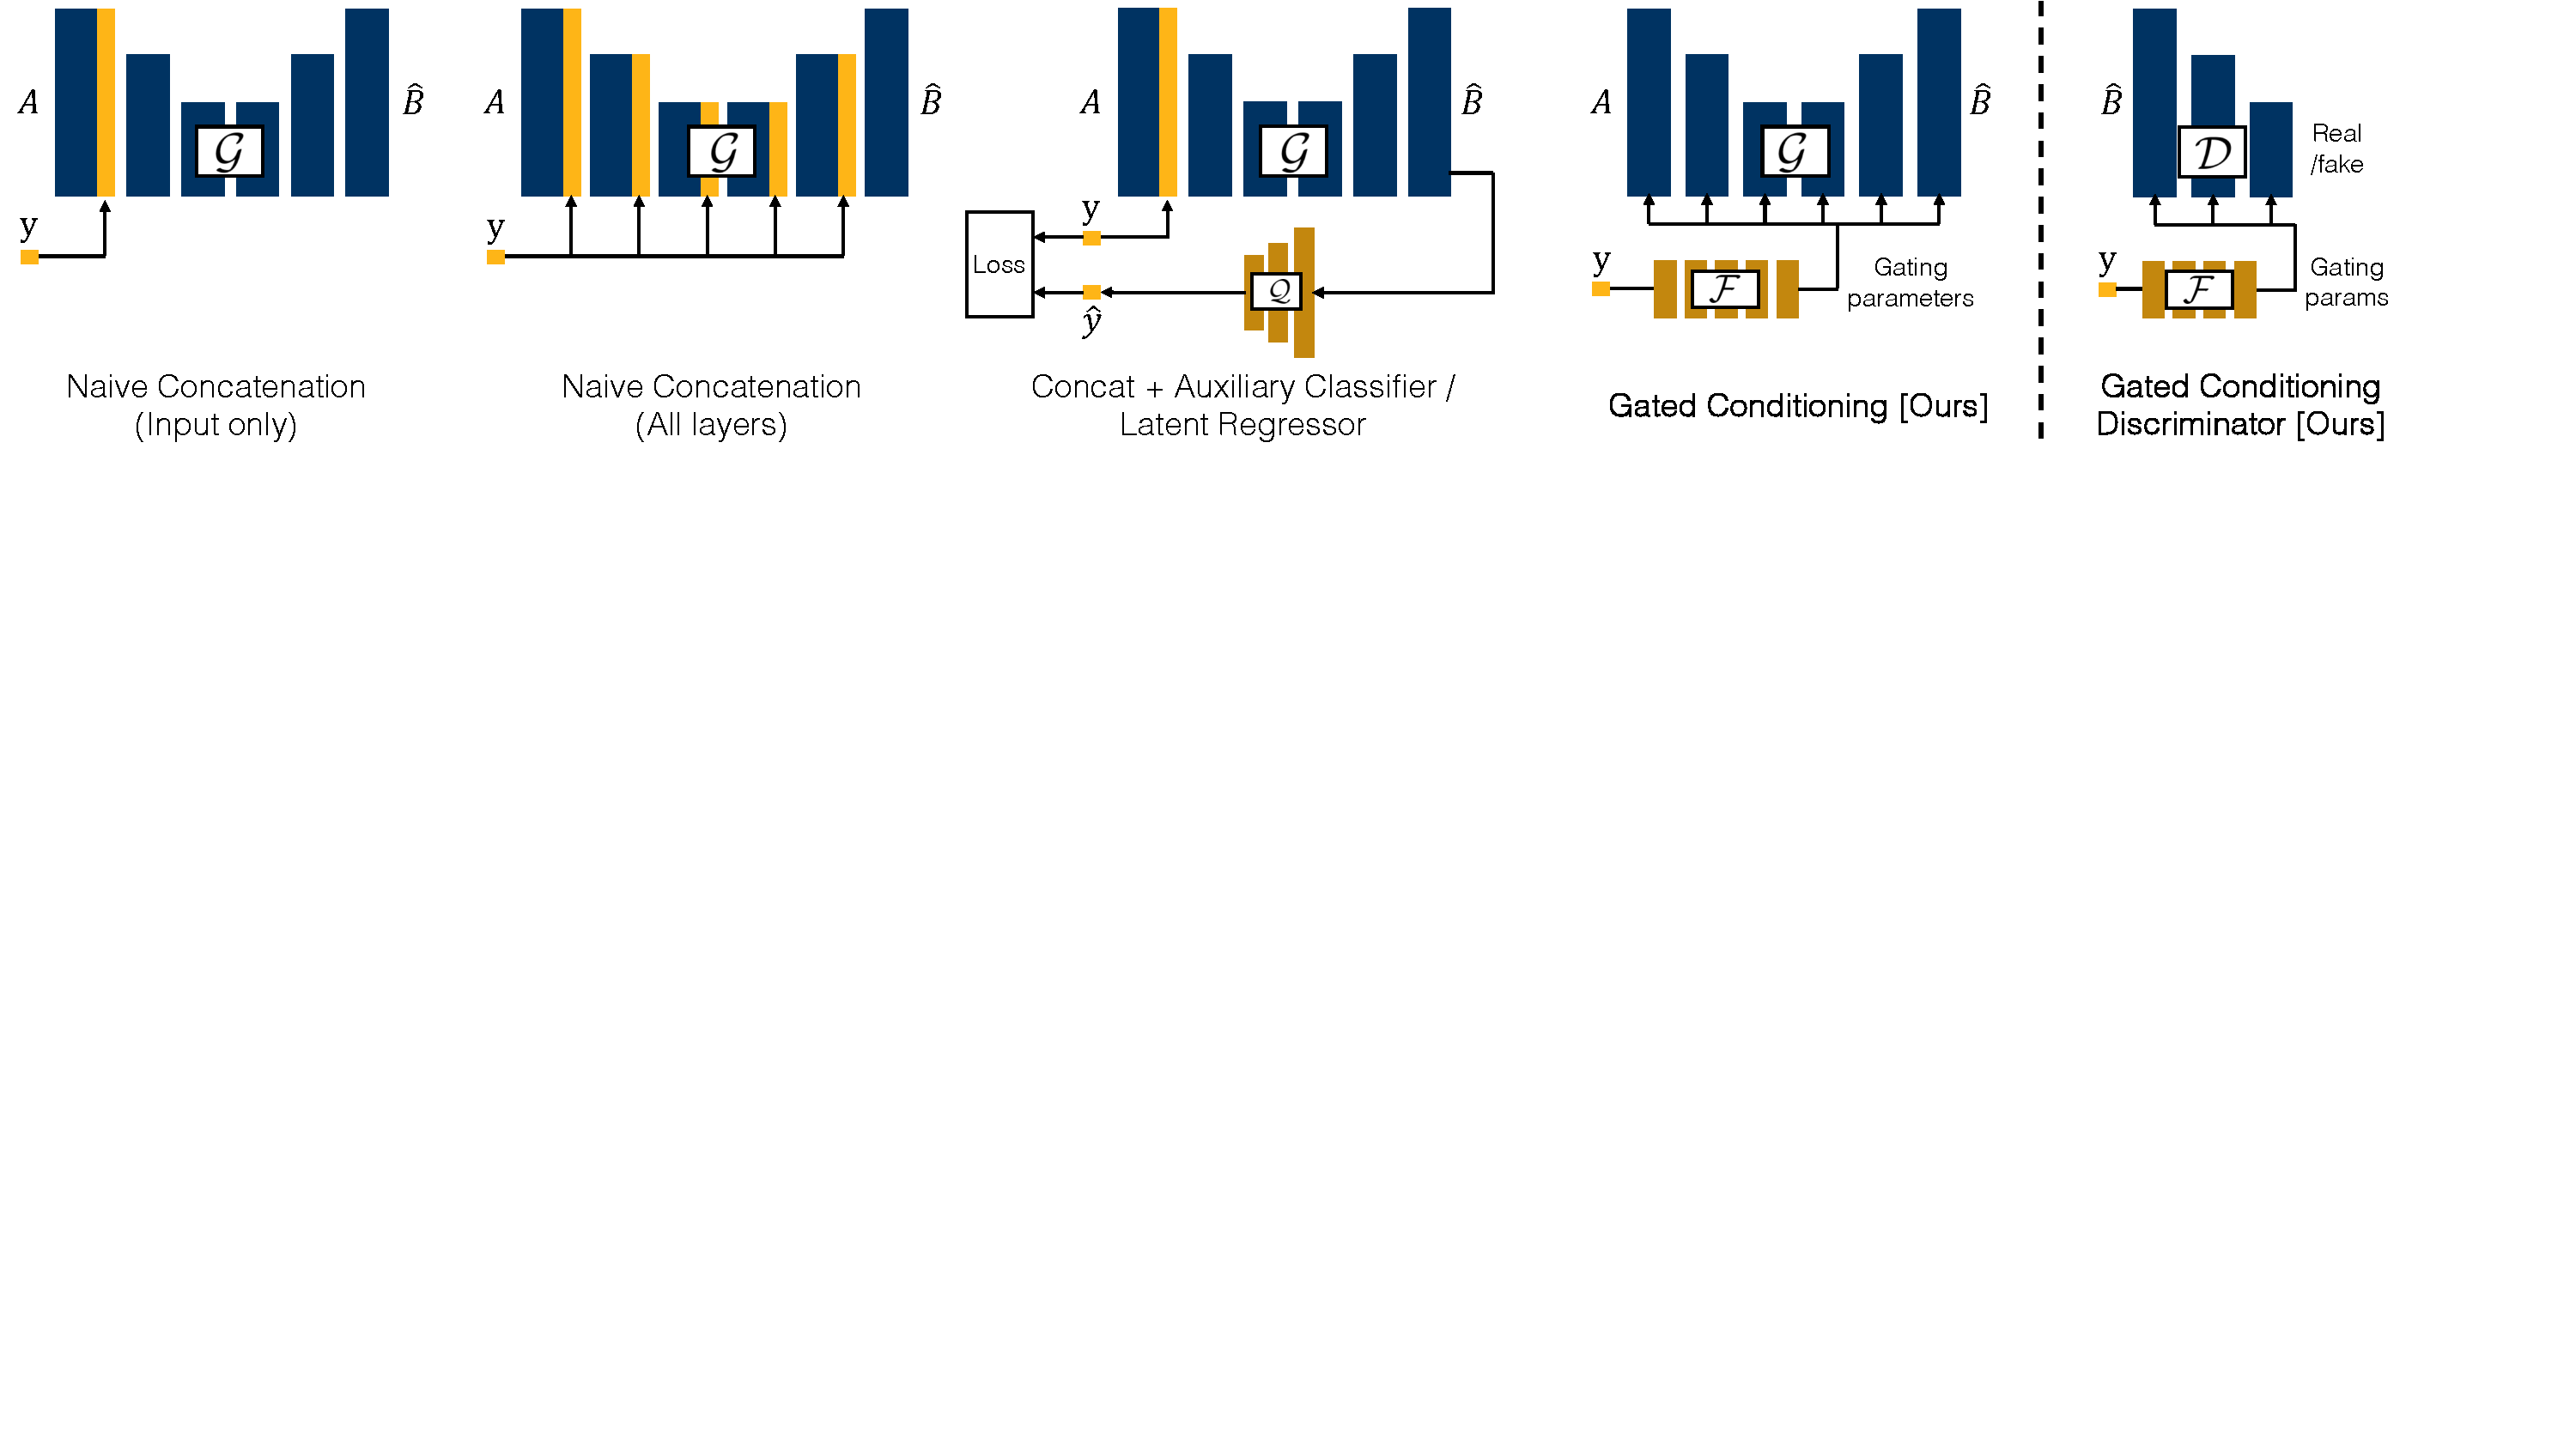
\includegraphics[width=\linewidth]{paper_images/arch_inject2.pdf}
    \caption{{\bf Conditioning injection variants.}
    The conditioner can be naively incorporated in a generator through simple concatenation in {\bf (left)} the input layer only or {\bf (mid-left)} in all layers. {\bf (mid)} The network can be further encouraged to use the conditioning through a learned network, using either a classification objective for categorical conditioning~\cite{odena2016conditional,chen2016infogan} or a regression objective for continuous conditioning. {\bf (Mid-right)} We train a network on the conditioner to predict parameters which guide softly-gated units in the main network. {\bf (Right)} These conditioning options can be correspondingly applied to a discriminator. We propose using soft-gating on the discriminator as well.\label{fig:arch-inj}
    \vspace{-2mm}
    }
    \vspace{-2mm}
\end{figure*}
\begin{figure*}[t]
\centering
\begin{tabular}{*{3}{c@{\hspace{3px}}}}
\textbf{Blockwise Gating} & \textbf{Channelwise Gating} \vspace{-1mm} & \\
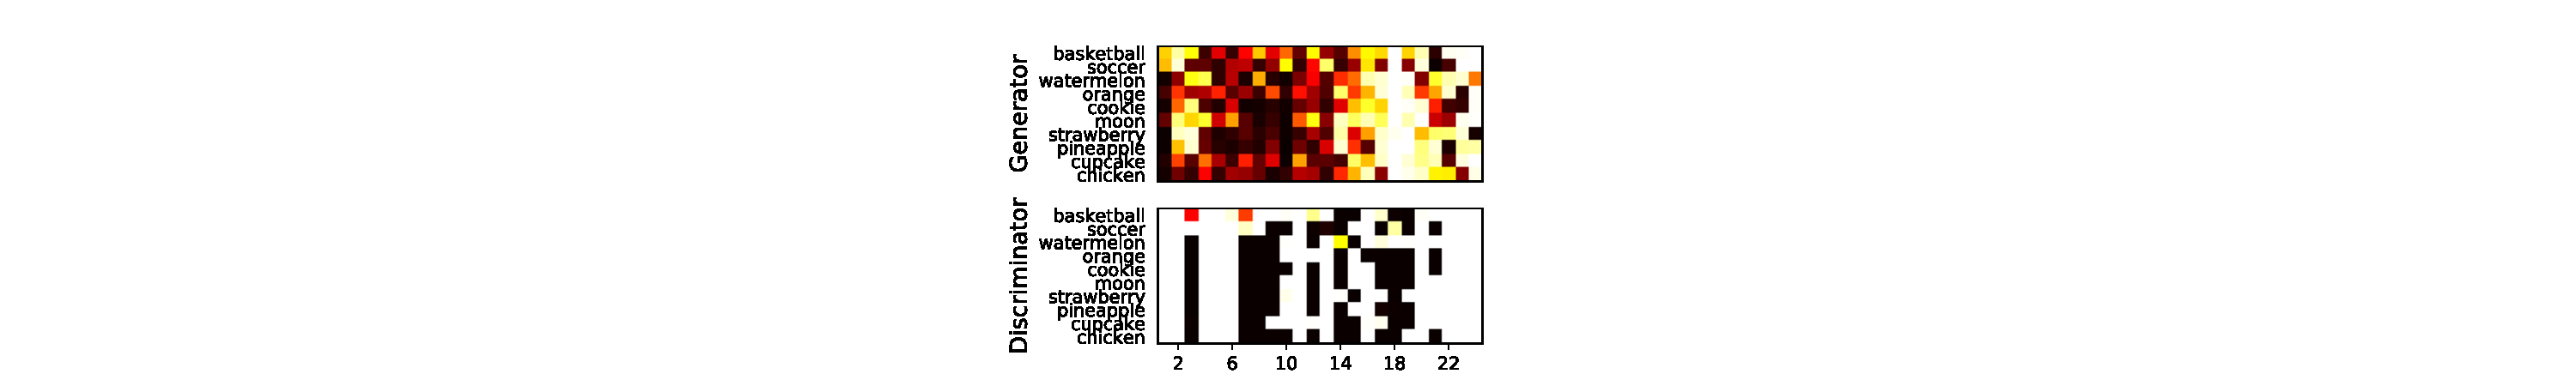
\includegraphics[height=3.35cm,trim={.15cm 0 0 .4cm}, clip]{paper_images/alphas_block.pdf} &
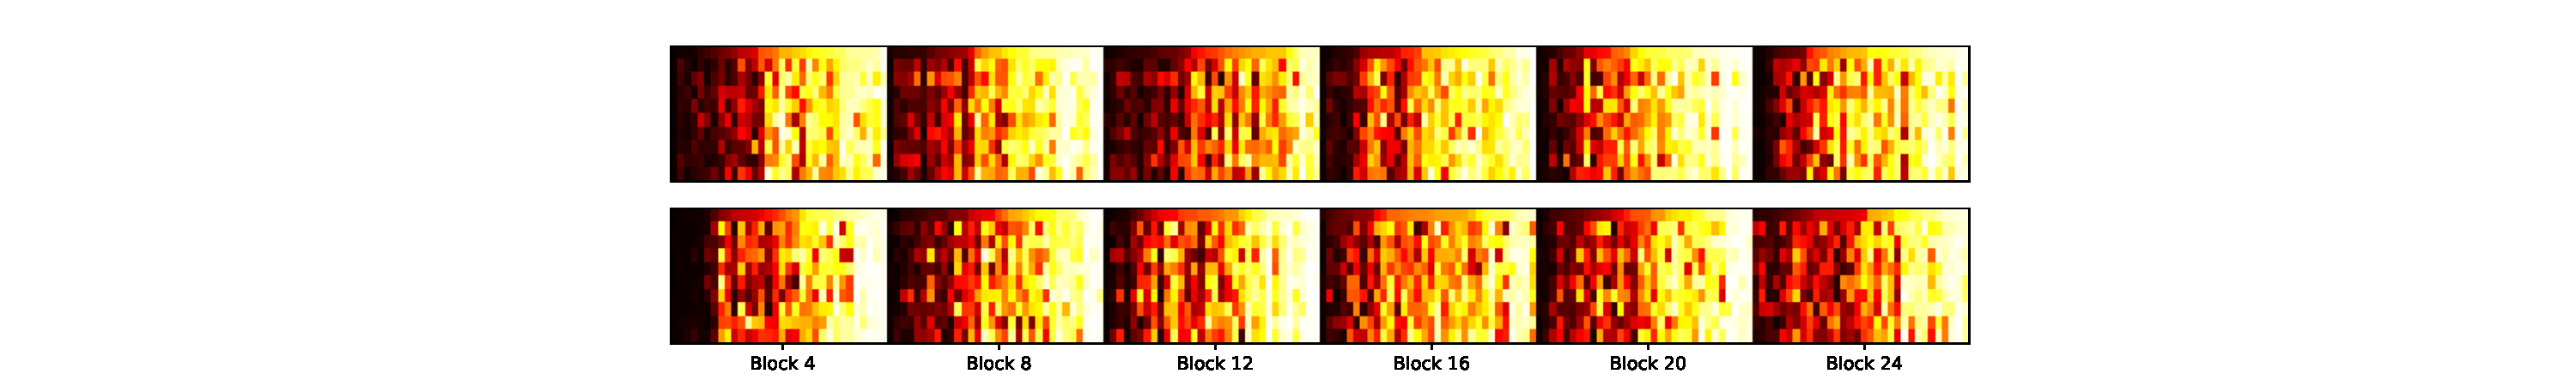
\includegraphics[height=3.35cm,trim={0 0 0 .4cm}, clip]{paper_images/alphas_chan.pdf} & 
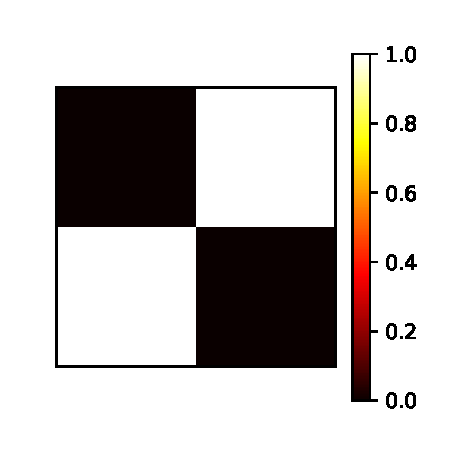
\includegraphics[height=3.35cm,trim={5.8cm 0 .2cm .4cm}, clip]{paper_images/alpha_legend.pdf}
\\
\end{tabular}
\vspace{-2mm}
\caption{\label{fig:alpha_heat}
\textbf{Learned gating parameters.} We show the soft-gating parameters for {\bf (left)} blockwise and {\bf (right)} channelwise gating for the {\bf (top)} generator and {\bf (bot)} discriminator. Black indicates
% $\alpha=0$, or
completely off, and white indicates
% $\alpha=1$, or 
completely on. For channelwise, a subset (every 4th) of blocks is shown. Within each block, channels are sorted in ascending order of the first category. The nonuniformity of each columns indicates that different channels are used more heavily for different classes.
\vspace{-3mm}
}
\vspace{-2mm}
\end{figure*}

% \begin{figure*}[t]
%     \centering
%     % 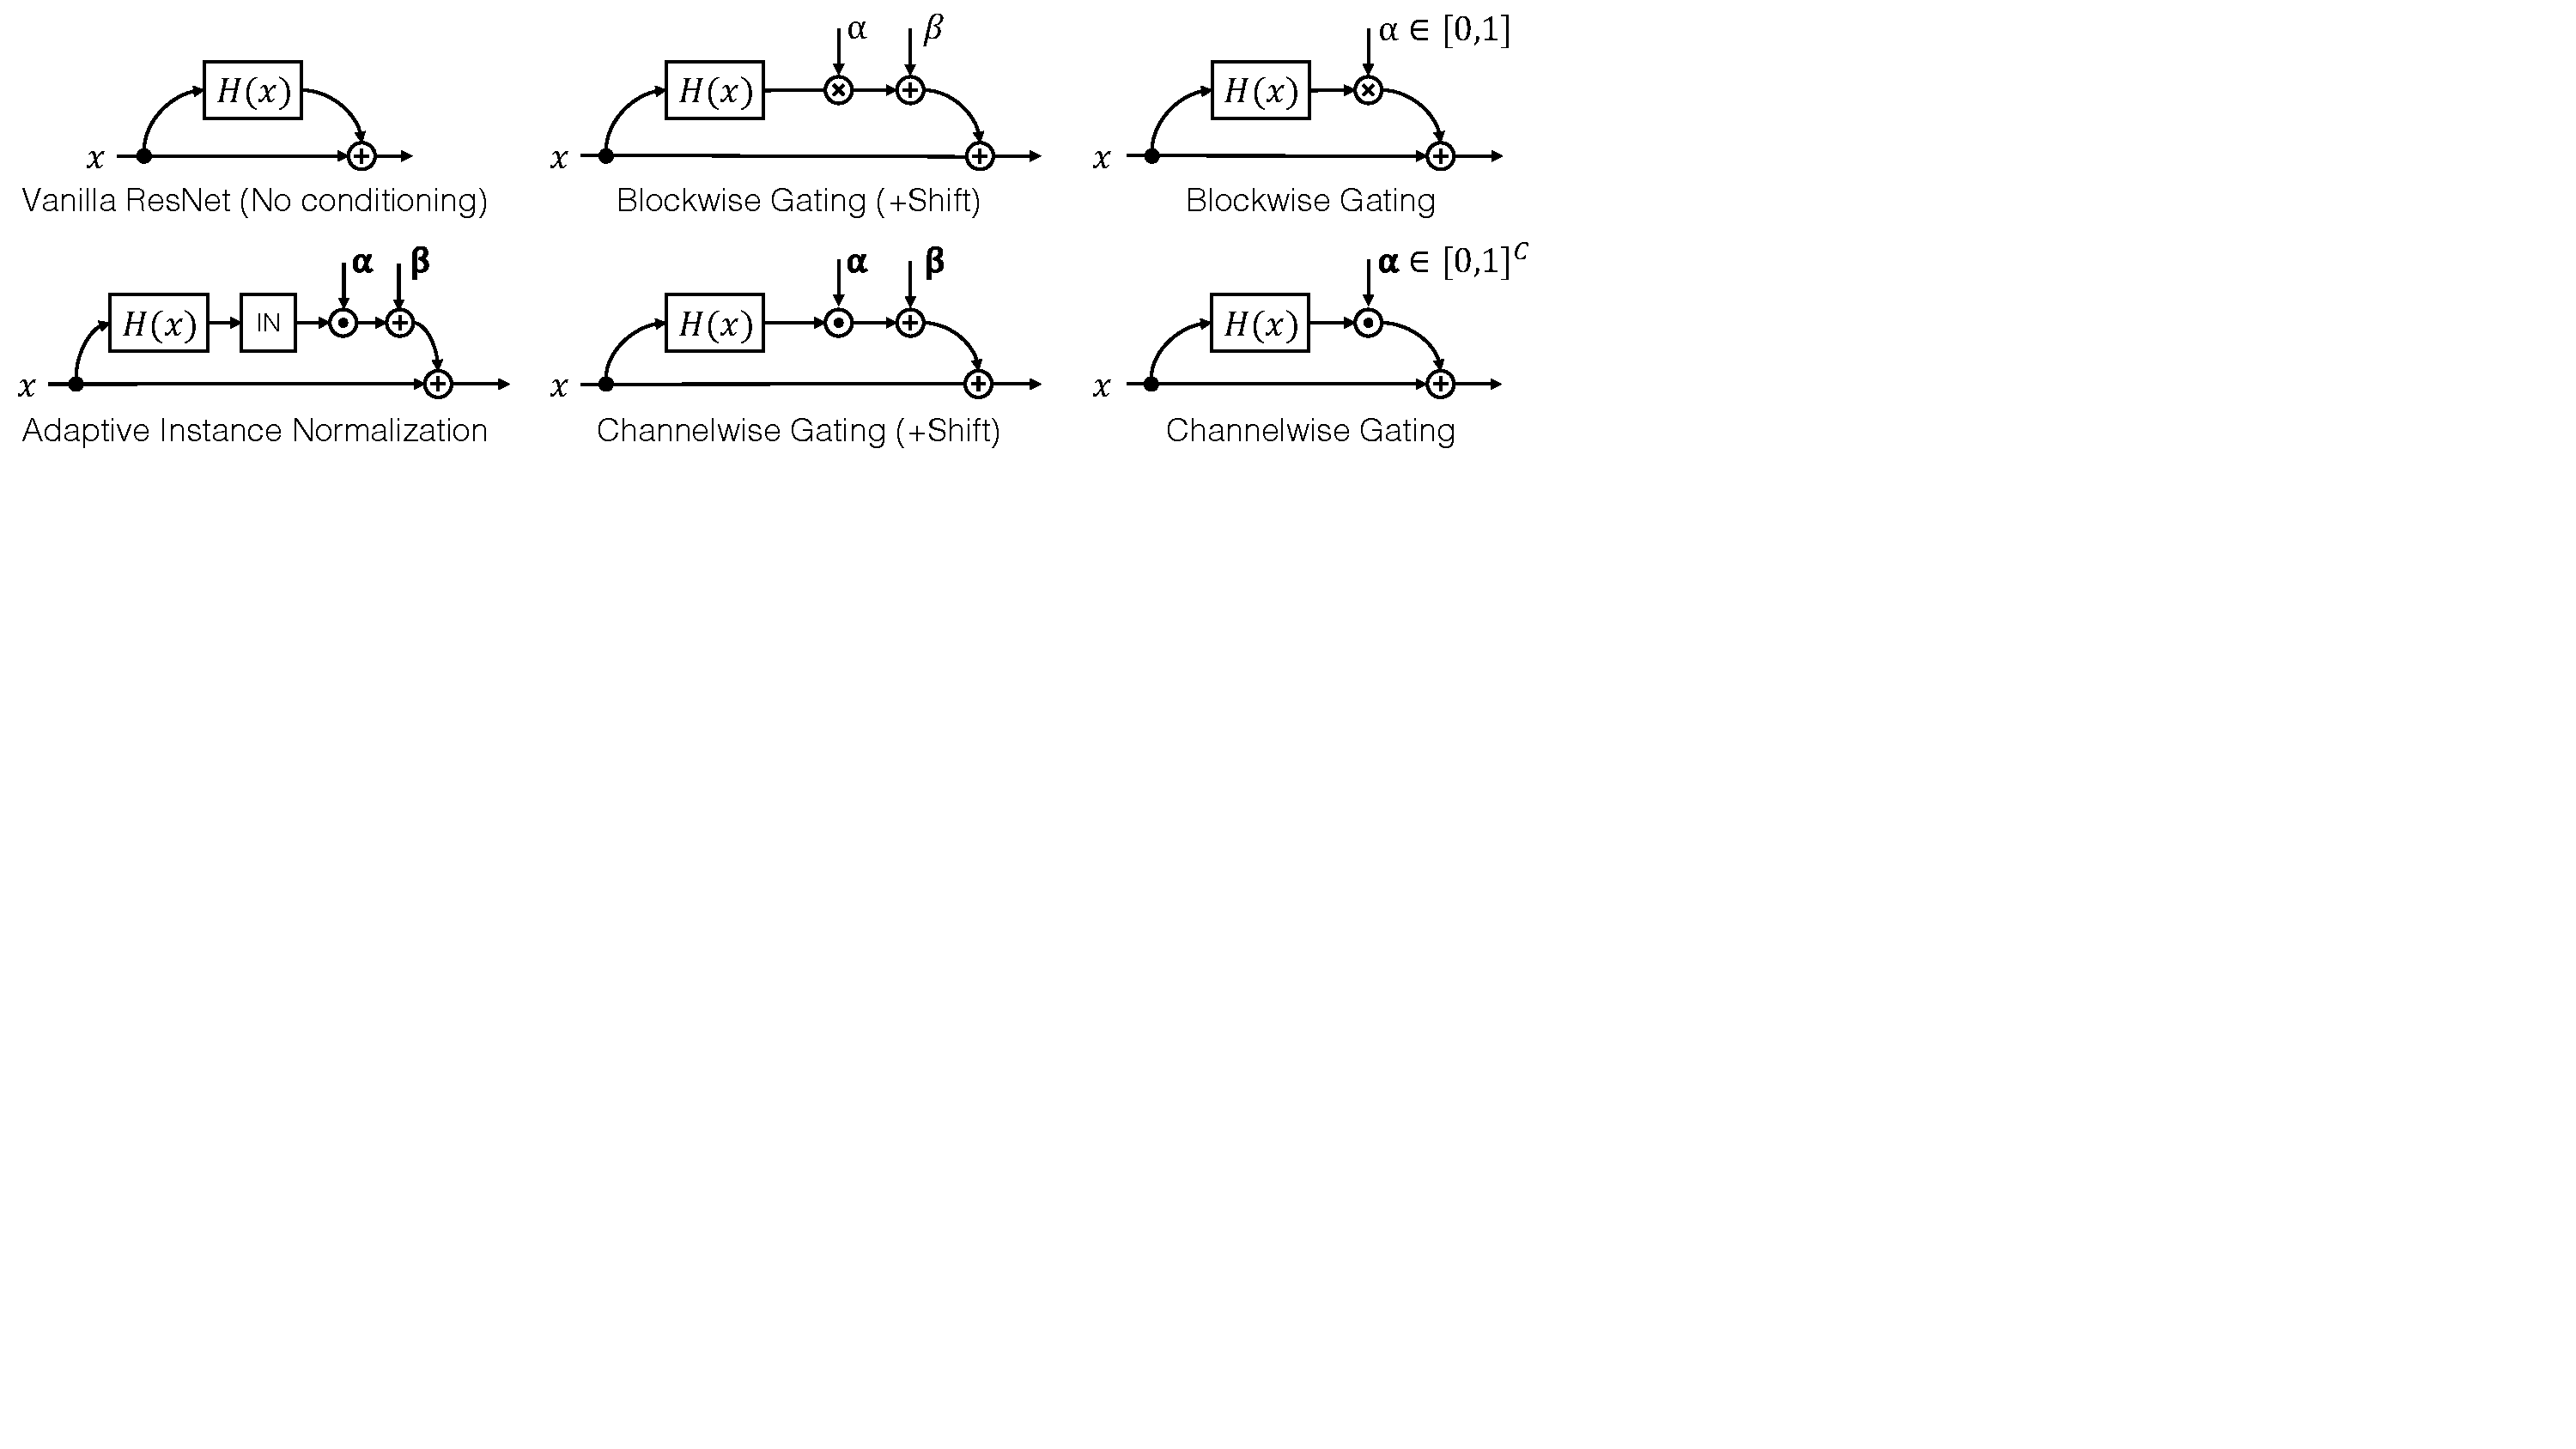
\includegraphics[width=\linewidth]{paper_images/arch_gate.pdf}
%     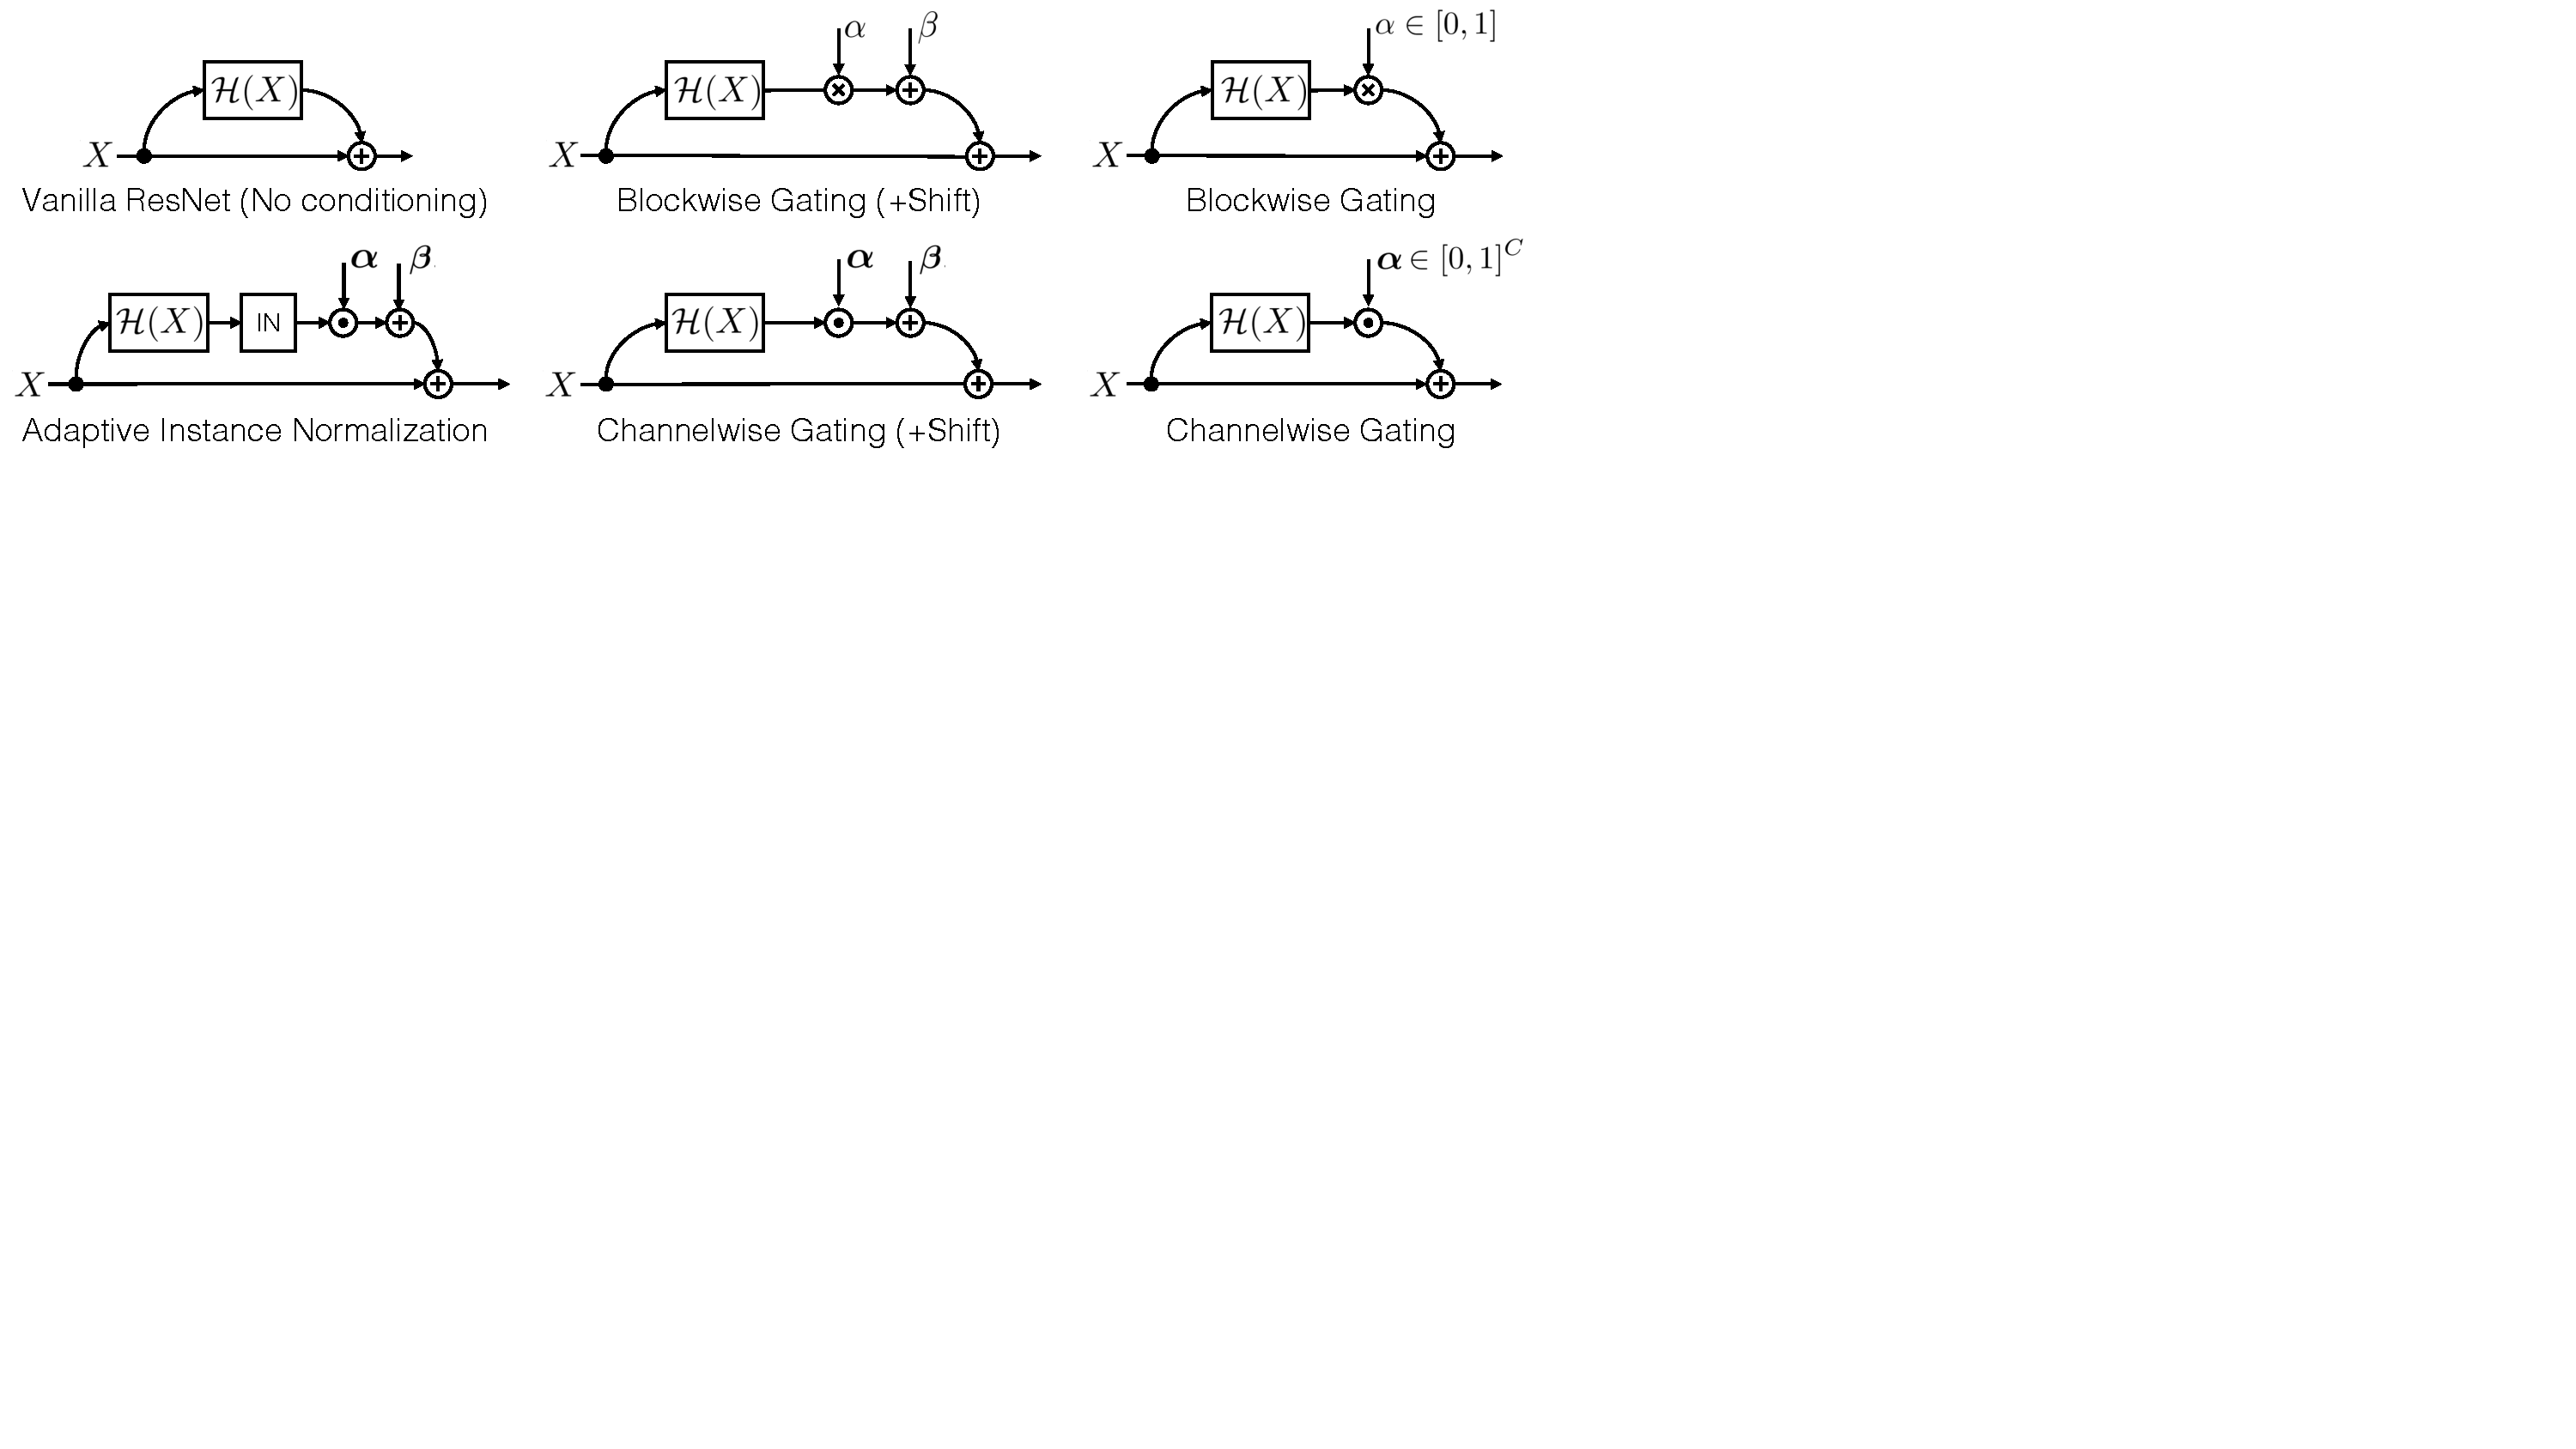
\includegraphics[width=.9\linewidth]{paper_images/arch_gate2.pdf}
%     \caption{
%     % {\bf Incorporating soft-gating into residual blocks.} \rz{Order got changed, may or may not need to add key for hadamard product}
%     {\bf (Top-left)} A ``vanilla" residual block without gated conditioning parameters modifies input tensor $X$ into $X+\mathcal{H}(X)$. Conditioning with concatenation uses this setup. {\bf (Top-mid)} The $\mathcal{H}(X)$ block is softly-gated by scalar parameter $\alpha$ and shift $\beta$. {\bf (Top-right)} Only the gating is used, without bias. {\bf (Bot-left)} Adaptive Instance Normalization~\cite{huang2017arbitrary} applies a channel-wise scaling and shifting after an instance normalization layer. {\bf (Bot-mid)} Channel-wise gating adds restrictions to the range of $\mbox{\boldmath $\alpha$}$. {\bf (Bot-right)} We find that channel-wise gating (without added bias) to empirically produce the best results.\label{fig:arch-gate}
%     \vspace{-2mm}
%     }
%     % \vspace{-4mm}
% \end{figure*}




% \section{1D Mixture of Gaussians Dataset}
% % In order to understand the behavior of the various residual blocks, we first perform a very simple synthetic experiment, much easier than generating high-dimensional complex images.
% We consider a 1D mixture of Gaussians with five components with modes at 10, 20, 60, 80 and 110, and standard deviations of 3, 3, 2, 2 and 1, respectively. While the first two modes overlap significantly, the fifth mode stands isolated as shown in Figure 6 of the main paper.
% % \figref{fig:onedexperiment}. 
% We train our Resnet block based GAN model using 1 million samples from this distribution and generate 1 million samples from the trained model. In order to compare the learned distribution with the ground truth distributions, we estimate the learned distribution by computing histograms over the data points. 
% %These histograms are carefully created using different bin sizes and the best bin (found to be 0.1) is chosen. 
% %The generated distribution from the trained model corresponds very closely to the ground truth distribution. 
% As shown in 
% % \figref{fig:onedexperiment}
% Figure 6 in the main paper, the generated distribution closely matches the ground truth one, and we can observe that  residual blocks focus on specific modes, which motivates our gating mechanism.


\section{1D Network Architecture}
% \ow{but why was this architecture chosen? did the normal ones in madgan/mode gan not work? what motivates the skinny resnet?} 
The architecture was designed hoping to reproduce some of the experiments performed by \cite{veit2016residual} by removing blocks and observing the resulting generated distribution, hence a design choice of having a deep network but keeping the neurons in each block lesser in order to reduce chances of overfitting/overparametrizing for a relatively simpler task. The interesting aspect was that although the network was deeper (16 layers of residual blocks) than required for similar experiments in MAD-GAN \cite{ghosh2017multi}, Mode Regularized GAN \cite{che2016mode} and Unrolled GAN \cite{metz2017unrolledGAN}, there were only 4 neurons in each residual block of the generator and discriminator (Tables~\ref{table:1d_G}~\&~\ref{table:1d_D}) compared to fully connected versions in which there consisted of connections between 256 neurons in the preceding layer to 256 neurons in the current layer. Thus although the number of parameters were much less, the network learned the distribution quite accurately. The architecture used in this experiment inspired the design of the skinny Resnet architecture as described later.

\begin{table}[ht]
\caption{\textbf{ResBlock}} % title of Table
\centering % used for centering table
\begin{tabular}{c} % centered columns (4 columns)
\toprule
\textbf{F(x)}\\\midrule
Linear\\ % inserting body of the table
ReLU() \\
Linear\\
\bottomrule %inserts single line
\end{tabular}
\label{table:resblock} % is used to refer this table in the text
\end{table}

\begin{table}[ht]
\caption{\textbf{Generator for 1D setting}} % title of Table
\centering % used for centering table
\begin{tabular}{l c c}
%  \hline
\toprule
\textbf{Layer} & \textbf{Neurons} & \textbf{Num Layers} \\ \midrule
Linear & 10 $\rightarrow$ 4 & 1  \\ %\midrule
ResBlock & 4 & 16 \\ 
Linear & 4$\rightarrow$ 1 & 1 \\ 
\bottomrule %inserts single line
\end{tabular}
\label{table:1d_G} % is used to refer this table in the text
\end{table}

% \begin{table}[ht]
% \caption{\textbf{Generator for 1D setting}} % title of Table
% \centering % used for centering table
% \begin{tabular}{c c} % centered columns (4 columns)
% \hline\hline %inserts double horizontal lines
% layer & num layers\\%heading
% \hline % inserts single horizontal line
% Linear(10,4) & 1\\ % inserting body of the table
% ResBlock(4) & 16 \\
% Linear(4,1) & 1 \\
% \hline %inserts single line
% \end{tabular}
% \label{table:1d_G} % is used to refer this table in the text
% \end{table}

% \begin{table}[ht]
% \caption{\textbf{Discriminator for 1D setting}} % title of Table
% \centering % used for centering table
% \begin{tabular}{c c} % centered columns (4 columns)
% \hline\hline %inserts double horizontal lines
% layer & num layers\\%heading
% \hline % inserts single horizontal line
% Linear(1,4) & 1\\ % inserting body of the table
% ResBlock(4) & 16 \\
% Linear(4,1) & 1 \\
% Sigmoid & 1 \\
% \hline %inserts single line
% \end{tabular}
% \label{table:1d_D} % is used to refer this table in the text
% \end{table}

\begin{table}[ht]
\caption{\textbf{Discriminator for 1D setting}} % title of Table
\centering % used for centering table
\begin{tabular}{l c c}
%  \hline
\toprule
\textbf{Layer} & \textbf{Neurons} & \textbf{Num Layers} \\ \midrule
Linear & 1 $\rightarrow$ 4 & 1  \\ %\midrule
ResBlock & 4 & 16 \\ 
Linear & 4 $\rightarrow$ 1 & 1 \\
Sigmoid & 1 & 1 \\
\bottomrule %inserts single line
\end{tabular}
\label{table:1d_D} % is used to refer this table in the text
\end{table}


\section{Outline$\rightarrow$Image Network Architecture}
The network architecture is based on our observations that deeper networks perform better capturing multi-modal data distributions. The second guiding principle in the design of the architecture is that the different blocks should have similar number of channels so that the gating hypernetwork can distribute the modes between the blocks efficiently. Finally, the residual blocks responsible for upsampling and downsampling were gated as well in order to allow more blocks to be gated and hence better fine-grained control on the generation process. 
\tabref{table:convresblock} shows the Convolution Residual Block which does not change the spatial resolution of the activation volume, 
\tabref{table:downconvresblock} shows the Downsampling Residual Block which reduces the activation volume to half the spatial resolution, 
\tabref{table:upconvresblock} shows the Upsampling Residual Block which increases the activation volume to twice the spatial resolution,  and in the case of gating (either block wise/channel-wise) the gating is applied on the $F(x)$ of each network. 
The shortcut branch represented in \tabref{table:upconvresblock} and \tabref{table:downconvresblock} represents the branch of the Resnet which is added to $F(x)$ branch. In these scenarios since the resolution of $x$ changes in $F(x)$ branch hence the shortcut also has a similar upsampling/downsampling layer.


\begin{table}[ht]
    \makegapedcells
        \centering % used for centering table
        \begin{tabular}{c} % centered columns (4 columns)
        % \hline\hline %inserts double horizontal lines
        \toprule
        \textbf{F(x)}\\%heading
        \midrule
        Conv2d \\
        InstanceNorm\\ % inserting body of the table
        ReLU() \\
        Conv2d \\
        InstanceNorm\\ % inserting body of the table
        ReLU() \\
        \bottomrule %inserts single line
        \end{tabular}
        \caption{\textbf{ConvResblock}} % title of Table
        \label{table:convresblock} % is used to refer this table in the text
\end{table}

\begin{table}
        \centering % used for centering table
        \begin{tabular}{c} % centered columns (4 columns)
        \toprule % \hline\hline %inserts double horizontal lines
        \textbf{F(x)}\\%heading
        \midrule % \hline
        Upsample (Nearest Neighbor) \\
        ReflectionPad \\
        Conv2d \\
        InstanceNorm\\ % inserting body of the table
        ReLU() \\
        Conv2d \\
        InstanceNorm\\ % inserting body of the table
        ReLU() \\
        \midrule % \hline %inserts single line
        \textbf{Shortcut Branch}\\
        \midrule % \hline 
        Upsample (Bilinear) \\
        ReflectionPad\\
        Conv2d \\
        \bottomrule % \hline
        \end{tabular}
        \caption{        \label{table:upconvresblock} \textbf{UpConvResblock}} % title of Table
\end{table}

\begin{table}
        \centering % used for centering table
        \begin{tabular}{c} % centered columns (4 columns)
        \toprule % \hline\hline %inserts double horizontal lines
        \textbf{F(x)}\\%heading
        \midrule
        Avgpool 2d \\
        ReflectionPad \\
        Conv2d \\
        InstanceNorm\\ % inserting body of the table
        ReLU() \\
        Conv2d \\
        InstanceNorm\\ % inserting body of the table
        ReLU() \\
        \midrule% \hline %inserts single line
        \textbf{Shortcut Branch}\\
        \midrule % \hline 
        Avgpool 2d \\
        ReflectionPad\\
        Conv2d \\
        \bottomrule% \hline
        \end{tabular}
        \caption{\label{table:downconvresblock} \textbf{DownConvResblock}} 
\end{table}


\begin{table}[ht]
\caption{\textbf{Gated Resnet G:Scribble Dataset}}
\centering % used for centering table
\begin{tabular}{l c c} % centered columns (4 columns)
\toprule% \hline
\textbf{Layer} & \textbf{Filter} & \textbf{Num Layers} \\
\midrule
Conv2d & 3 $\rightarrow$ 32 & 1\\
InstanceNorm & 32 & 1 \\ % inserting body of the table
ReLU() & 32 & 1\\
\hdashline% \hline %inserts single line
\textbf{Gated}-ConvResBlock & 32 & 3\\
\textbf{Gated}-DownConvResBlock & 32 & 3\\
\textbf{Gated}-ConvResBlock & 32 & 12\\
\textbf{Gated}-UpConvResBlock & 32 & 3\\
\textbf{Gated}-ConvResBlock & 32 & 3\\
\hdashline
Conv2d & 32$\rightarrow$3 & 1 \\
Tanh() & 3 & 1 \\
\bottomrule% \hline
\end{tabular}
\label{table:resnet_g_scribble} % is used to refer this table in the text
\end{table}

\begin{table}[ht]
\caption{\textbf{Gated Resnet D:Scribble Dataset}}
\centering % used for centering table
\begin{tabular}{l c c} % centered columns (4 columns)
\toprule% \hline
\textbf{Layer} & \textbf{Filter} & \textbf{Num Layers} \\
\midrule
Conv2d & 6 $\rightarrow$ 32 & 1\\
\hdashline% \hline %inserts single line
\textbf{Gated}-ConvResBlock & 32 & 3\\
\textbf{Gated}-DownConvResBlock & 32 & 4\\
\textbf{Gated}-ConvResBlock & 32 & 17\\
\hdashline
Conv2d & 32$\rightarrow$1 & 1 \\
Sigmoid() & 1 & 1 \\
\bottomrule% \hline
\end{tabular}
\label{table:resnet_d_scribble} % is used to refer this table in the text
\end{table}


% \begin{table}[ht]
% \caption{\textbf{Gated Resnet G:Multi-Task Dataset}}
% \centering % used for centering table
% \begin{tabular}{l c c} % centered columns (4 columns)
% \toprule% \hline
% \textbf{Layer} & \textbf{Filter} & \textbf{Num Layers} \\
% \midrule
% Conv2d & 3 $\rightarrow$ 64 & 1\\
% InstanceNorm & 64 & 1 \\ % inserting body of the table
% ReLU() & 64 & 1\\
% \hdashline% \hline %inserts single line
% \textbf{Gated}-ConvResBlock & 64 & 3\\
% \textbf{Gated}-DownConvResBlock & 64 & 3\\
% \textbf{Gated}-ConvResBlock & 64 & 4\\
% \textbf{Gated}-UpConvResBlock & 64 & 3\\
% \textbf{Gated}-ConvResBlock & 64 & 3\\
% \hdashline
% Conv2d & 64$\rightarrow$3 & 1 \\
% Tanh() & 3 & 1 \\
% \bottomrule% \hline
% \end{tabular}
% \label{table:resnet_g_multitask} % is used to refer this table in the text
% \end{table}

% \begin{table}[ht]
% \caption{\textbf{Gated Resnet D:Multi-Task Dataset}}
% \centering % used for centering table
% \begin{tabular}{l c c} % centered columns (4 columns)
% \toprule% \hline
% \textbf{Layer} & \textbf{Filter} & \textbf{Num Layers} \\
% \midrule
% Conv2d & 6 $\rightarrow$ 64 & 1\\
% \hdashline% \hline %inserts single line
% \textbf{Gated}-ConvResBlock & 64 & 3\\
% \textbf{Gated}-DownConvResBlock & 64 & 4\\
% \textbf{Gated}-ConvResBlock & 64 & 9\\
% \hdashline
% Conv2d & 64$\rightarrow$1 & 1 \\
% Sigmoid() & 1 & 1 \\
% \bottomrule% \hline
% \end{tabular}
% \label{table:resnet_d_multitask} % is used to refer this table in the text
% \end{table}


\subsection{Gating Hypernetwork:}
The gating hypernetwork was also designed using Resnet blocks, we used 1D convolutions in the Resnet block \tabref{table:resblock1D} to reduce the number of parameters and to use BatchNormalization to speed up the training of the network responsible for the prediction of gating. The class conditioning is first passed through an embedding layer to obtain a representation of the class which could be further processed by the Resnet blocks. The same network is used for the various forms of gating. In case of block wise gating the number of outputs $dim^{gate}$ for this network is equal to the number of blocks used in the main network, in the case of an affine transformation the network predicts an equal number of biases for each of the block. In case of channel-wise gating the number of predicted parameters $dim^{gate}$ is equal to $num^{channels}\times num^{blocks}$ since each residual block consists of equal number of channels in each it helps to ease the training of the gating hypernetwork. The $\alpha$ was constrained between 0 and 1 to mimic whether to select a block or to reject the block while the $\beta$ in the case of affine transformation was restricted between -1 and 1. In the case of standard AdaIN, the parameters are unrestricted but it did not work in that setting and the AdaIN parameters had to be constrained between -1 and 1 in order for the network to perform well. 

\begin{table}[ht]
\caption{\textbf{ResBlock1D}} % title of Table
\centering % used for centering table
\begin{tabular}{c} % centered columns (4 columns)
\toprule
\textbf{F(x)}\\\midrule
Conv1D\\ % inserting body of the table
BatchNorm1D\\
ReLU \\
Conv1D\\
BatchNorm1D\\
ReLU \\
\bottomrule %inserts single line
\end{tabular}
\label{table:resblock1D} % is used to refer this table in the text
\end{table}

\begin{figure*}[t]
    \centering
    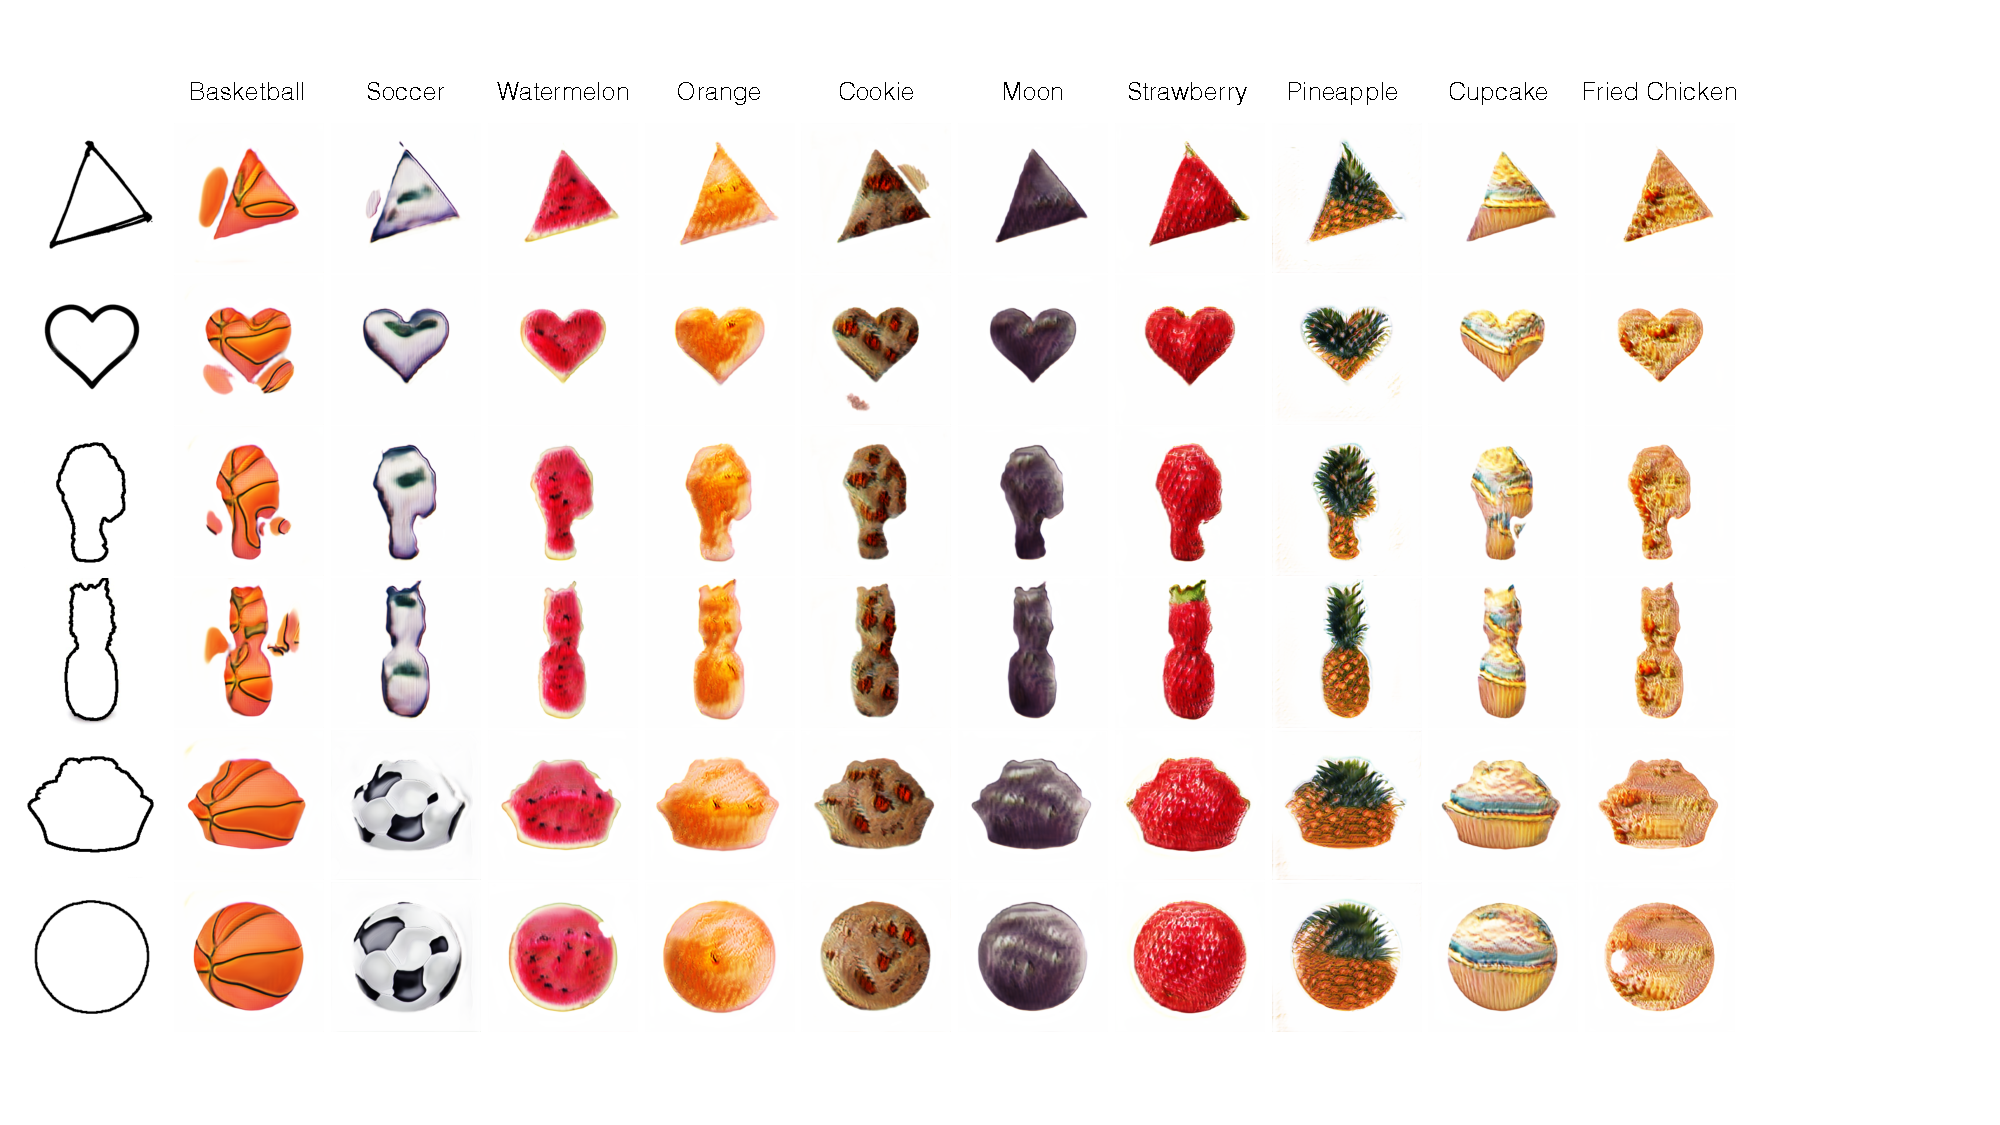
\includegraphics[width=\linewidth,trim={0 0 4.5cm 0},clip]{paper_images/supplementary_grid_channel.pdf}
    % 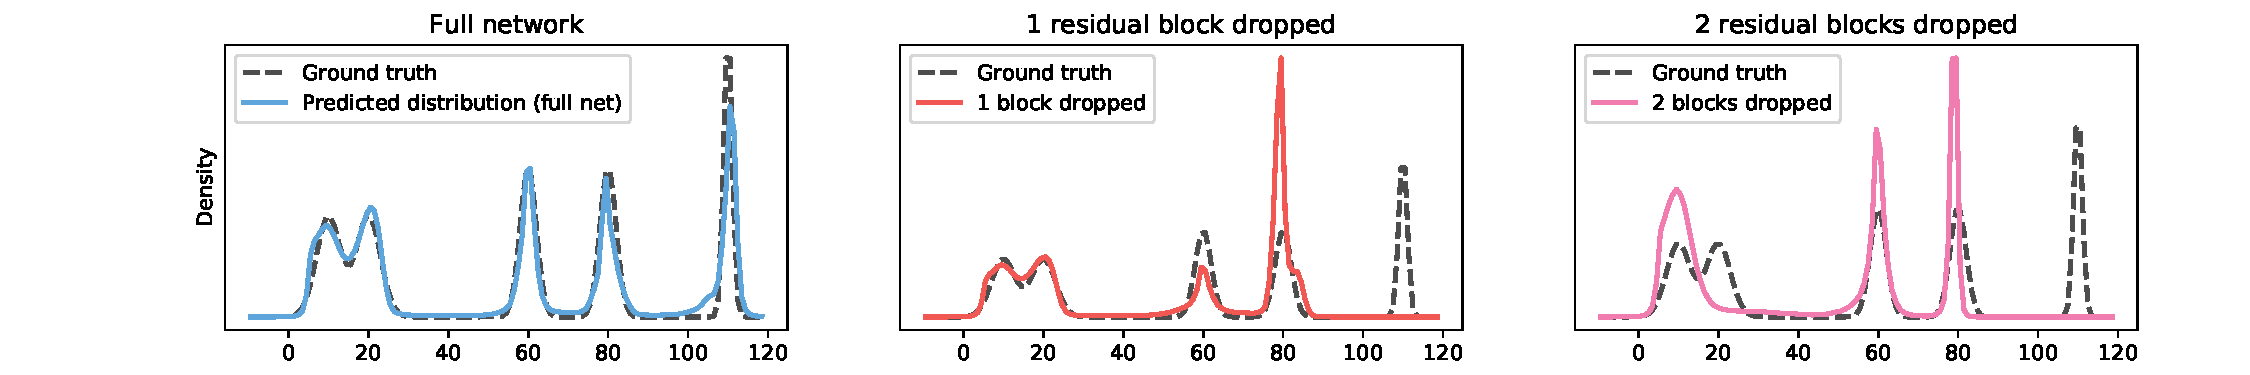
\includegraphics[width=\linewidth]{paper_images/mog.pdf}
    \caption{{\bf Channel-Wise Gating:} We observe that the technique extends to not only the shapes it was trained on but can also generate images for some input shapes corresponding to other classes and to the extreme can generate images for certain shapes it never encountered during training such as the triangle and heart were directly downloaded from the internet. }
    \label{fig:channel_shapes}
    \vspace{-3mm}
\end{figure*}


\begin{table}[ht]
\caption{\textbf{Gating Hyper Network} $dim^{gate}$ is the number of blocks in the case of Block Wise Gating and the number of channels in the case of Channel Wise Gating. In case of affine its twice of each since the $\beta$ is of the same dimension }
\centering % used for centering table
\begin{tabular}{l c c} % centered columns (4 columns)
\toprule% \hline
\textbf{Layer} & \textbf{Filter/Shape} & \textbf{Num Layers} \\
\midrule
Embedding & $dim^{embed}$ & 1 \\
Conv1d & 1 $\rightarrow$ 16 & 1\\
% \hdashline% \hline %inserts single line
ResBlock1D & 16 & 16\\
Reshape & 16$\times dim^{embed}$ & 1\\
Linear & 16$\times dim^{embed} \rightarrow dim^{gate} $& 1\\
\bottomrule% \hline
\end{tabular}
\label{table:resnet_gating} % is used to refer this table in the text
\end{table}


% \section{Multimodal Generation (InfoGAN with variations)}
% \label{sec:multimodal}


% Inter-class variation, also called diversity, is a significant challenge in GAN image generation applications. 
% In the pix2pix setting, as shown by previous works \cite{ghosh2017multi} and \cite{zhu2017toward} even the InfoGAN (cLR in \cite{zhu2017toward}) setup was not able to produce meaningful variations (irrespective of the variations in the conditioning), and additional generators or cyclical losses were required to produce meaningful variations in the generated images. 
% With our gating mechanism, we show that we can create meaningful variations, using just the InfoGAN objective.
% This can be seen in the results \figref{fig:infogan_gate} and from the LPIPS metric \cite{zhang2018unreasonable} in  Table. \ref{table:infogan_lpips} which measures the diversity among the generations in the feature space of a standard Imagenet classifier.
% % Since InfoGAN maximizes mutual information, we argue that gating provides a mechanism to effectively optimize it by making the conditioning an active part of the generation process (refer Sec.~\ref{sec:infoGAN}).

% \begin{figure}[h]
%     \centering
%     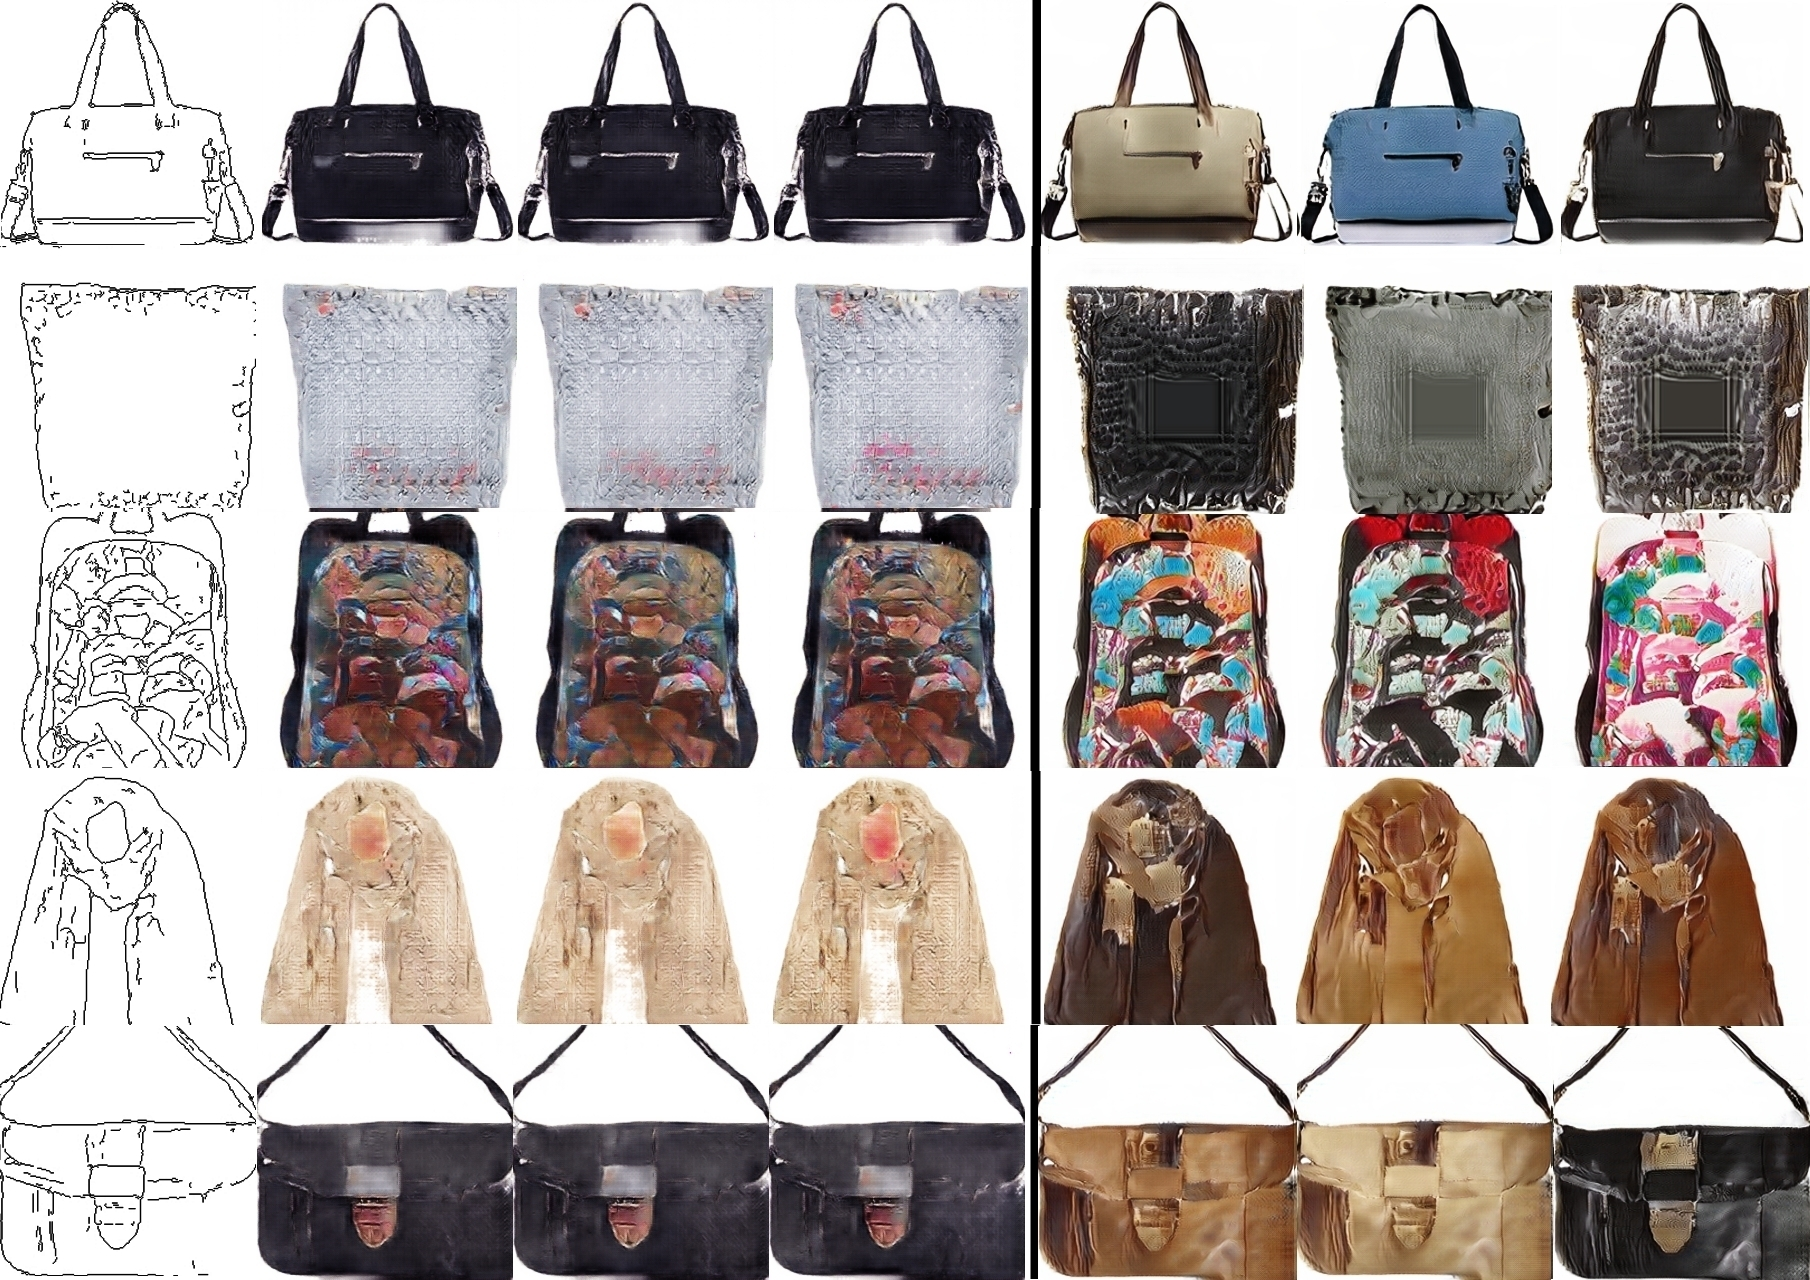
\includegraphics[width=\linewidth]{infogan.jpg}
%     \caption{{\bf Edges$\rightarrow$Handbags qualitative examples.} Naive Conditioning of InfoGAN fails (left) while gating (right) succeeds in producing diverse generations.
%     \vspace{-5mm}
%     }\label{fig:infogan_gate}
%     % \vspace{-2mm}
% \end{figure}
% \begin{table}[h]
%     \centering
%         \begin{tabular}{l c}
%         % \hline
%         \toprule
%         \textbf{Model} & \textbf{LPIPS Distance} \\ \midrule
%         Random Real Images & $0.3665 \pm 0.0053$ \\ \midrule
%         BicycleGAN~\cite{zhu2017toward} & $0.1374 \pm 0.0005$  \\ \midrule
%         Concat(In) &  $0.0432 \pm 0.0002$ \\
%         Concat(All) & $0.0159 \pm 0.0004$ \\ \cdashline{1-2}
%         ChannelGate [Ours] & $0.0964 \pm 0.0003$  \\
%         \bottomrule %inserts single line
%         \end{tabular}
%     \caption{\label{table:infogan_lpips} {\bf Edges$\rightarrow$Handbags Diversity.} LPIPSv0.1~\cite{zhang2018unreasonable} distance between randomly generated handbags, given the same edge map, as proposed in~\cite{zhu2016generative}. Given the same architecture, gating achieves higher diversity than concatenation.}
% \end{table}



% % \begin{figure*}[t]
% %     \centering
% %     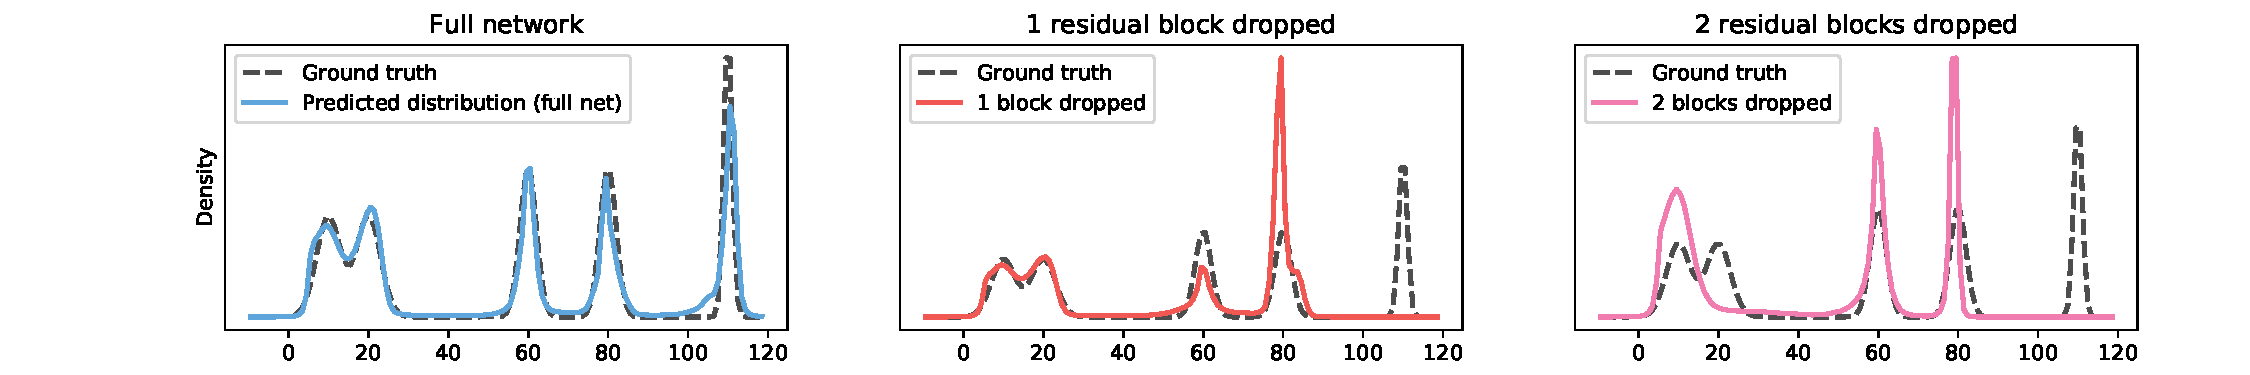
\includegraphics[width=\linewidth,trim={2.6cm 0 1.8cm 0},clip]{paper_images/mog.pdf}
% %     % \includegraphics[width=\linewidth]{paper_images/mog.pdf}
% %     \caption{{\bf 1D Mixture of Gaussians.} {\bf (Left)} Samples from a residual network (blue-dotted) closely approximate the training distribution (black). {\bf (Mid)} Removing one residual block removes one mode of the predicted distribution. {\bf (Right)} Removing two blocks drops two modes. Note that samples stay mostly ``on-manifold" of the ground truth distribution. {\bf Note:} This is a reproduction of Figure 2 from the main paper, it is included here for completeness.
% %     \vspace{-2mm}
% %     }\label{fig:onedexperiment}
% %     \vspace{-3mm}
% % \end{figure*}

% \subsection{Multimodal Generations: Architecture}
% The network architectures used in this setting are very similar to the ones used for the outline $\rightarrow$ image generation with some small differences. The discriminator and the Q network responsible for the maximization of mutual information are not gated in this case since the class labels are not provided to the discriminator or the Q network. The number of blocks and channels in each block in the case of the generator are more than the case of scribble dataset. The gating hypernetwork also differs slightly since the sampled variables are not only one-hot encoding but a combination of one-hot and gaussian variables, hence we directly use it and bypass the embedding layer.

% \begin{table}[ht]
% \caption{\textbf{Gating Hyper Network(InfoGAN)}
% % nsalient(12) are the number of variables representing
% We have $C=2$ continuous and $K=10$ discrete latent variables. Variable $dim^{gate}$ is the number of channels which are gated. }
% \centering % used for centering table
% \begin{tabular}{l c c} % centered columns (4 columns)
% \toprule% \hline
% \textbf{Layer} & \textbf{Filter/Shape} & \textbf{Num Layers} \\
% \midrule
% Reshape & $K+C$ & 1 \\
% Conv1d & 1 $\rightarrow$ 16 & 1\\
% % \hdashline% \hline %inserts single line
% ResBlock1D & 16 & 16\\
% Reshape & $16\times (K+C)$ & 1\\
% Linear & $16\times (K+C) \rightarrow dim^{gate} $& 1\\
% \bottomrule% \hline
% \end{tabular}
% \label{table:resnet_gating_infogan} % is used to refer this table in the text
% \end{table}

% \begin{table}[ht]
% \caption{\textbf{Gated Resnet G:InfoGAN}}
% \centering % used for centering table
% \begin{tabular}{l c c} % centered columns (4 columns)
% \toprule% \hline
% \textbf{Layer} & \textbf{Filter} & \textbf{Num Layers} \\
% \midrule
% Conv2d & 3 $\rightarrow$ 64 & 1\\
% InstanceNorm & 64 & 1 \\ % inserting body of the table
% ReLU() & 64 & 1\\
% \hdashline% \hline %inserts single line
% \textbf{Gated}-ConvResBlock & 64 & 3\\
% \textbf{Gated}-DownConvResBlock & 64 & 3\\
% \textbf{Gated}-ConvResBlock & 64 & 20\\
% \textbf{Gated}-UpConvResBlock & 64 & 3\\
% \textbf{Gated}-ConvResBlock & 64 & 3\\
% \hdashline
% Conv2d & 64$\rightarrow$3 & 1 \\
% Tanh() & 3 & 1 \\
% \bottomrule% \hline
% \end{tabular}
% \label{table:resnet_g_infogan} % is used to refer this table in the text
% \end{table}


% \begin{table}[ht]
% \caption{\textbf{Resnet D:Infogan}}
% \centering % used for centering table
% \begin{tabular}{l c c} % centered columns (4 columns)
% \toprule% \hline
% \textbf{Layer} & \textbf{Filter} & \textbf{Num Layers} \\
% \midrule
% Conv2d & 6 $\rightarrow$ 64 & 1\\
% \hdashline% \hline %inserts single line
% ConvResBlock & 64 & 3\\
% DownConvResBlock & 64 & 4\\
% ConvResBlock & 64 & 25\\
% \hdashline
% Conv2d & 64$\rightarrow$1 & 1 \\
% Sigmoid() & 1 & 1 \\
% \bottomrule% \hline
% \end{tabular}
% \label{table:resnet_d_infogan} % is used to refer this table in the text
% \end{table}

% \begin{table}[ht]
% \caption{\textbf{Resnet Q:Infogan}}
% \centering % used for centering table
% \begin{tabular}{l c c} % centered columns (4 columns)
% \toprule% \hline
% \textbf{Layer} & \textbf{Filter/Shape} & \textbf{Num Layers} \\
% \midrule
% Conv2d & 6 $\rightarrow$ 64 & 1\\
% \hdashline% \hline %inserts single line
% ConvResBlock & 64 & 3\\
% DownConvResBlock & 64 & 4\\
% ConvResBlock & 64 & 25\\
% \hdashline
% Conv2d & 64$\rightarrow$1 & 1 \\
% Reshape & 225 & 1 \\
% \midrule
% \textbf{Discrete Branch} \\
% \midrule
% Linear & 225 $\rightarrow$ 10 & 1 \\
% \midrule
% \textbf{Continuous Branch($\mu$)} \\
% \midrule
% Linear & 225 $\rightarrow$ 2 & 1 \\
% \midrule
% \textbf{Continuous Branch($\sigma$)} \\
% \midrule
% Linear & 225 $\rightarrow$ 2 & 1 \\
% \bottomrule% \hline
% \end{tabular}
% \label{table:resnet_q_infogan} % is used to refer this table in the text
% \end{table}

% \begin{table}[ht]
% \caption{\textbf{Gated Resnet D:Scribble Dataset}} % title of Table
% \centering % used for centering table
% \begin{tabular}{c} % centered columns (4 columns)
% \hline
% Conv2d(6,64,kernel=3,stride=1,padding=1) \\
% \hline %inserts single line
% 3xGatedConvResBlock(64) \\
% 4xDownGatedConvResBlock(64) \\
% 17xGatedConvResBlock(64) \\
% \hline
% Conv2d(64,1,kernel=3,stride=1,padding=1) \\
% Sigmoid() \\
% \hline
% \end{tabular}
% \label{table:resnet_d_scribble} % is used to refer this table in the text
% \end{table}

\section{Unusual Shapes for Various Classes:}

% \begin{figure*}[t]
%     \centering
%     \includegraphics[width=\linewidth,trim={0 0 4.5cm 0},clip]{paper_images/supplementary_grid_block.pdf}
%     % \includegraphics[width=\linewidth]{paper_images/mog.pdf}
%     \caption{{\bf Block-Wise Gating:} We observe that the technique extends to not only the shapes it was trained on but can also generate images for some input shapes corresponding to other classes and to the extreme can generate images for certain shapes it never encountered during training such as the triangle and heart were directly downloaded from the internet. }
%     \label{fig:block_shapes}
%     \vspace{-3mm}
% \end{figure*}

As evident from \figref{fig:channel_shapes} 
% ,\figref{fig:block_shapes} 
the gated generative techniques extend to shapes it never was shown while training. 

\section{Subset of Comparison of Results:}

We show the results of our various gating mechanisms along with all the baselines reported in the paper on the Scribble Dataset's subset of test images. These images were the ones used for Amazon Mechanical Turk and the evaluation metrics reported in the paper.
\href{http://www.robots.ox.ac.uk/~arnabg/all_results_supplementary/index.html}{Comparison of our technique vs all baselines}

\section{Distribution of Alphas:}
The histogram of the distribution of the various alphas for the block-wise setting and the channel-wise setting are shown in \figref{fig:alpha_hist}. Even without a sparsity constraint the alphas are pushed nearer the extremes rather than clustering near intermediate values. The effect is more starkly demonstrated in the case of the block wise gating, with the channel wise gating parameters being more evenly distributed.
\begin{figure*}[t]
    \centering
    \includegraphics[width=\linewidth]{alpha_hist.pdf}
    % \includegraphics[width=\linewidth]{paper_images/mog.pdf}
    \caption{As we see from the distribution of the various alphas they are closer to the extremes (0 or 1) rather than the intermediate values, quite similar in the case of the channel wise gating as well }
    \label{fig:alpha_hist}
    \vspace{-3mm}
\end{figure*}

\section{Interpolations:}
In order to judge the robustness of the trained models and to analyze the differences between the naive concatenation techniques compared with our gating mechanisms we conduct some inter-class interpolations. As we can see from \figref{fig:inter_watermelon_cookie}, \figref{fig:inter_orange_basketball}, \figref{fig:inter_cookie_moon} and \figref{fig:inter_orange_cupcake} that our gating mechanisms produce smooth transitions between classes while the case of naive concatenation techniques failing to generate basketball at all, thus failing at interpolating between basketball and orange.


{\small
\bibliographystyle{ieee}
\bibliography{src/gatedblocks}
}

\begin{figure*}[t]
    \centering
    \includegraphics[width=\linewidth]{interpolation-watermelon-cookie.pdf}
    % \includegraphics[width=\linewidth]{paper_images/mog.pdf}
    \caption{{\bf Cookie $\rightarrow$ Watermelon:} As evident from the interpolation the gating produces much smoother transitions than simple concatenation techniques }
    \label{fig:inter_watermelon_cookie}
    \vspace{-3mm}
\end{figure*}


\begin{figure*}[t]
    \centering
    \includegraphics[width=\linewidth]{interpolation-orange-basketball.pdf}
    % \includegraphics[width=\linewidth]{paper_images/mog.pdf}
    \caption{ {\bf Basketball $\rightarrow$ Orange:} A failure case of the simple conditioning technique, it never generates basketball and hence is not able to interpolate between basketball and orange. }
    \label{fig:inter_orange_basketball}
    \vspace{-3mm}
\end{figure*}

\begin{figure*}[t]
    \centering
    \includegraphics[width=\linewidth]{interpolation-cookie-moon.pdf}
    % \includegraphics[width=\linewidth]{paper_images/mog.pdf}
    \caption{ {\bf Moon $\rightarrow$ Cookie:} Interpolation between moon and cookie }
    \label{fig:inter_cookie_moon}
    \vspace{-3mm}
\end{figure*}

\begin{figure*}[t]
    \centering
    \includegraphics[width=\linewidth]{interpolation-orange-cupcake.pdf}
    % \includegraphics[width=\linewidth]{paper_images/mog.pdf}
    \caption{ {\bf Orange $\rightarrow$ Cupcake:} Interpolation between orange and cupcake, in the case of the baseline concat mechanism there's an abrupt transition from orange to cupcake while the transition is much smoother in the case of gated mechanisms }
    \label{fig:inter_orange_cupcake}
    \vspace{-3mm}
\end{figure*}




\begin{figure*}[t]
\centering
\begin{tabular}{*{2}{c@{\hspace{3px}}}}
% \textbf{Blockwise Gating} & \textbf{Channelwise Gating} \vspace{-1mm} \\
% \includegraphics[height=3.35cm,trim={0 0 0 .4cm}, clip]{paper_images/alphas_chan_1.pdf} & 
\includegraphics[height=3.15cm,trim={6.0cm 0 7.6cm .4cm}, clip]{paper_images/alphas_chan_0.pdf} & 
\includegraphics[height=3.15cm,trim={5.8cm 0 .2cm .4cm}, clip]{paper_images/alpha_legend.pdf}
\\
\includegraphics[height=3.15cm,trim={6.0cm 0 7.6cm .4cm}, clip]{paper_images/alphas_chan_8.pdf} & 
\includegraphics[height=3.15cm,trim={5.8cm 0 .2cm .4cm}, clip]{paper_images/alpha_legend.pdf}
\\
\includegraphics[height=3.15cm,trim={6.0cm 0 7.6cm .4cm}, clip]{paper_images/alphas_chan_16.pdf} & 
\includegraphics[height=3.15cm,trim={5.8cm 0 .2cm .4cm}, clip]{paper_images/alpha_legend.pdf}
\\

\end{tabular}
\vspace{-2mm}
\caption{\label{fig:alpha_heat}
\textbf{Learned channel-wise gating parameters.} We show the soft-gating parameters for channelwise gating for the {\bf (top)} generator and {\bf (bot)} discriminator. Black indicates
% $\alpha=0$, or
completely off, and white indicates
% $\alpha=1$, or 
completely on. We show all 24 blocks. This is an extension of Fig. 6 in the main paper. The nonuniformity of each columns indicates that different channels are used more heavily for different classes.
\vspace{-3mm}
}
\vspace{-2mm}
\end{figure*}


\end{document}

\end{document}




% \begin{figure*}%[ht!]
%     \centering
%     \addSubFigTenth{acgan_baseline_all/basketball_11_real_A}{}{fig:basketball_scribble} 
%     \addSubFigTenth{acgan_baseline_all/chicken_2_real_A}{}{fig:chicken_scribble} 
%     \addSubFigTenth{acgan_baseline_all/cookie_13_real_A}{}{fig:cookie_scribble}
%     \addSubFigTenth{acgan_baseline_all/cupcake_27_real_A}{}{fig:cupcake_scribble}
%     \addSubFigTenth{acgan_baseline_all/moon_15_real_A}{}{fig:moon_scribble}
%     \addSubFigTenth{acgan_baseline_all/basketball_11_fake_B}{}{fig:basketball_img} 
%     \addSubFigTenth{acgan_baseline_all/chicken_2_fake_B}{}{fig:chicken_img} 
%     \addSubFigTenth{acgan_baseline_all/cookie_13_fake_B}{}{fig:cookie_img}
%     \addSubFigTenth{acgan_baseline_all/cupcake_27_fake_B}{}{fig:cupcake_img}
%     \addSubFigTenth{acgan_baseline_all/moon_15_fake_B}{}{fig:moon_img}
%     \addSubFigTenth{acgan_baseline_all/orange_17_real_A}{}{fig:orange_scribble} 
%     \addSubFigTenth{acgan_baseline_all/pineapple_2_real_A}{}{fig:pineapple_scribble} 
%     \addSubFigTenth{acgan_baseline_all/soccer_18_real_A}{}{fig:soccer_scribble}
%     \addSubFigTenth{acgan_baseline_all/strawberry_1_real_A}{}{fig:strawberry_scribble}
%     \addSubFigTenth{acgan_baseline_all/watermelon_17_real_A}{}{fig:watermelon_scribble}
%     \addSubFigTenth{acgan_baseline_all/orange_17_fake_B}{}{fig:orange_img} 
%     \addSubFigTenth{acgan_baseline_all/pineapple_2_fake_B}{}{fig:pineapple_img} 
%     \addSubFigTenth{acgan_baseline_all/soccer_18_fake_B}{}{fig:soccer_img}
%     \addSubFigTenth{acgan_baseline_all/strawberry_1_fake_B}{}{fig:strawberry_img}
%     \addSubFigTenth{acgan_baseline_all/watermelon_17_fake_B}{}{fig:watermelon_img}
%     \caption{ACGAN baseline with Input Provided to all layers of Generator}
%     \label{fig:scribble_pix2pix}
%     \vspace{-3mm}
% \end{figure*}


% \begin{figure*}%[ht!]
%     \centering
%     \addSubFigTenth{channel_gated/basketball_11_real_A}{}{fig:basketball_scribble} 
%     \addSubFigTenth{channel_gated/chicken_2_real_A}{}{fig:chicken_scribble} 
%     \addSubFigTenth{channel_gated/cookie_13_real_A}{}{fig:cookie_scribble}
%     \addSubFigTenth{channel_gated/cupcake_27_real_A}{}{fig:cupcake_scribble}
%     \addSubFigTenth{channel_gated/moon_15_real_A}{}{fig:moon_scribble}
%     \addSubFigTenth{channel_gated/basketball_11_fake_B}{}{fig:basketball_img} 
%     \addSubFigTenth{channel_gated/chicken_2_fake_B}{}{fig:chicken_img} 
%     \addSubFigTenth{channel_gated/cookie_13_fake_B}{}{fig:cookie_img}
%     \addSubFigTenth{channel_gated/cupcake_27_fake_B}{}{fig:cupcake_img}
%     \addSubFigTenth{channel_gated/moon_15_fake_B}{}{fig:moon_img}
%     \addSubFigTenth{channel_gated/orange_17_real_A}{}{fig:orange_scribble} 
%     \addSubFigTenth{channel_gated/pineapple_2_real_A}{}{fig:pineapple_scribble} 
%     \addSubFigTenth{channel_gated/soccer_18_real_A}{}{fig:soccer_scribble}
%     \addSubFigTenth{channel_gated/strawberry_1_real_A}{}{fig:strawberry_scribble}
%     \addSubFigTenth{channel_gated/watermelon_17_real_A}{}{fig:watermelon_scribble}
%     \addSubFigTenth{channel_gated/orange_17_fake_B}{}{fig:orange_img} 
%     \addSubFigTenth{channel_gated/pineapple_2_fake_B}{}{fig:pineapple_img} 
%     \addSubFigTenth{channel_gated/soccer_18_fake_B}{}{fig:soccer_img}
%     \addSubFigTenth{channel_gated/strawberry_1_fake_B}{}{fig:strawberry_img}
%     \addSubFigTenth{channel_gated/watermelon_17_fake_B}{}{fig:watermelon_img}
%     \caption{Gated (Channel/Alpha) Results}
%     \label{fig:scribble_pix2pix}
%     \vspace{-3mm}
% \end{figure*}


% \begin{figure*}%[ht!]
%     \centering
%     \addSubFigSixthLabel{channel_gated/basketball_11_real_A}{Basketball}{fig:basketball_input} 
%     \addSubFigSixth{channel_gated/basketball_11_fake_B}{fig:basketball_ours} 
%     \addSubFigSixth{block_gated/basketball_11_fake_B}{fig:basketball_block}
%     \addSubFigSixth{channel_gated_affine/basketball_11_fake_B}{fig:basketball_channel_affine}
%     \addSubFigSixth{block_gated_affine/basketball_11_fake_B}{fig:basketball_block_affine}
%     \addSubFigSixth{adain/basketball_11_fake_B}{fig:basketball_adain}
    
%     \addSubFigSixthLabel{channel_gated/soccer_18_real_A}{Soccer ball}{fig:soccer_input}
%     \addSubFigSixth{channel_gated/soccer_18_fake_B}{fig:soccer_ours} 
%     \addSubFigSixth{block_gated/soccer_18_fake_B}{fig:soccer_block}
%     \addSubFigSixth{channel_gated_affine/soccer_18_fake_B}{fig:soccer_channel_affine}
%     \addSubFigSixth{block_gated_affine/soccer_18_fake_B}{fig:soccer_block_affine}
%     \addSubFigSixth{adain/soccer_18_fake_B}{fig:soccer_adain}
    
%     \addSubFigSixthLabel{channel_gated/moon_15_real_A}{Moon}{fig:moon_input}
%     \addSubFigSixth{channel_gated/moon_15_fake_B}{fig:moon_ours} 
%     \addSubFigSixth{block_gated/moon_15_fake_B}{fig:moon_block}
%     \addSubFigSixth{channel_gated_affine/moon_15_fake_B}{fig:moon_channel_affine}
%     \addSubFigSixth{block_gated_affine/moon_15_fake_B}{fig:moon_block_affine}
%     \addSubFigSixth{adain/moon_15_fake_B}{fig:moon_adain}
    
    
%     \addSubFigSixthLabel{channel_gated/cookie_13_real_A}{Cookie}{fig:cookie_input}
%     \addSubFigSixth{channel_gated/cookie_13_fake_B}{fig:cookie_ours} 
%     \addSubFigSixth{block_gated/cookie_13_fake_B}{fig:cookie_block}
%     \addSubFigSixth{channel_gated_affine/cookie_13_fake_B}{fig:cookie_channel_affine}
%     \addSubFigSixth{block_gated_affine/cookie_13_fake_B}{fig:cookie_block_affine}
%     \addSubFigSixth{adain/cookie_13_fake_B}{fig:cookie_adain}
    
    
%     \addSubFigSixthLabel{channel_gated/orange_17_real_A}{Orange}{fig:orange_input}
%     \addSubFigSixth{channel_gated/orange_17_fake_B}{fig:orange_ours} 
%     \addSubFigSixth{block_gated/orange_17_fake_B}{fig:orange_block}
%     \addSubFigSixth{channel_gated_affine/orange_17_fake_B}{fig:orange_channel_affine}
%     \addSubFigSixth{block_gated_affine/orange_17_fake_B}{fig:orange_block_affine}
%     \addSubFigSixth{adain/orange_17_fake_B}{fig:orange_adain}
    
%     \addSubFigSixthLabel{channel_gated/watermelon_17_real_A}{Watermelon}{fig:watermelon_input}
%     \addSubFigSixth{channel_gated/watermelon_17_fake_B}{fig:watermelon_ours} 
%     \addSubFigSixth{block_gated/watermelon_17_fake_B}{fig:watermelon_block}
%     \addSubFigSixth{channel_gated_affine/watermelon_17_fake_B}{fig:watermelon_channel_affine}
%     \addSubFigSixth{block_gated_affine/watermelon_17_fake_B}{fig:watermelon_block_affine}
%     \addSubFigSixth{adain/watermelon_17_fake_B}{fig:watermelon_adain}
    
%     \addSubFigSixthLabel{channel_gated/cupcake_27_real_A}{Cupcake}{fig:cupcake_input}
%     \addSubFigSixth{channel_gated/cupcake_27_fake_B}{fig:cupcake_ours} 
%     \addSubFigSixth{block_gated/cupcake_27_fake_B}{fig:cupcake_block}
%     \addSubFigSixth{channel_gated_affine/cupcake_27_fake_B}{fig:cupcake_channel_affine}
%     \addSubFigSixth{block_gated_affine/cupcake_27_fake_B}{fig:cupcake_block_affine}
%     \addSubFigSixth{adain/cupcake_27_fake_B}{fig:cupcake_adain}
    
    
%     \addSubFigSixthLabel{channel_gated/strawberry_1_real_A}{Strawberry}{fig:strawberry_input}
%     \addSubFigSixth{channel_gated/strawberry_1_fake_B}{fig:strawberry_ours} 
%     \addSubFigSixth{block_gated/strawberry_1_fake_B}{fig:strawberry_block}
%     \addSubFigSixth{channel_gated_affine/strawberry_1_fake_B}{fig:strawberry_channel_affine}
%     \addSubFigSixth{block_gated_affine/strawberry_1_fake_B}{fig:strawberry_block_affine}
%     \addSubFigSixth{adain/strawberry_1_fake_B}{fig:strawberry_adain}
    
%     \addSubFigSixthLabel{channel_gated/chicken_2_real_A}{Fried Chicken}{fig:chicken_input}
%     \addSubFigSixth{channel_gated/chicken_2_fake_B}{fig:chicken_ours} 
%     \addSubFigSixth{block_gated/chicken_2_fake_B}{fig:chicken_block}
%     \addSubFigSixth{channel_gated_affine/chicken_2_fake_B}{fig:chicken_channel_affine}
%     \addSubFigSixth{block_gated_affine/chicken_2_fake_B}{fig:chicken_block_affine}
%     \addSubFigSixth{adain/chicken_2_fake_B}{fig:chicken_adain}
    
%     \caption{Various Gating Mechanisms}
%     \label{fig:multi-task_cityscapes}
%     \vspace{-3mm}
% \end{figure*}